\documentclass[11pt]{article}%
\usepackage{geometry}%
\geometry{a4paper,
  lmargin=2cm,rmargin=2cm,tmargin=2.5cm,bmargin=2.5cm}

\usepackage{array}
\usepackage{paralist}

\usepackage[svgnames, usenames, dvipsnames]{xcolor}
\xdefinecolor{RecColor}{named}{Aqua}
\xdefinecolor{IncColor}{named}{Aqua}
\xdefinecolor{ImpColor}{named}{PaleGreen}

% \usepackage{frcursive}

\usepackage{adjustbox}

%%%%%%%%%%%
\newcommand{\cRB}[1]{{\color{Red} \pmb{#1}}} %
\newcommand{\cR}[1]{{\color{Red} {#1}}} %
\newcommand{\cBB}[1]{{\color{Blue} \pmb{#1}}}
\newcommand{\cB}[1]{{\color{Blue} {#1}}}
\newcommand{\cGB}[1]{{\color{LimeGreen} \pmb{#1}}}
\newcommand{\cG}[1]{{\color{LimeGreen} {#1}}}

%%%%%%%%%%

\usepackage{diagbox} %
\usepackage{colortbl} %
\usepackage{multirow} %
\usepackage{pgf} %
\usepackage{environ} %
\usepackage{fancybox} %
\usepackage{textcomp} %
\usepackage{marvosym} %

%%%%%%%%%% pour pouvoir faire des dashedline dans les tableaux
\usepackage{arydshln}

%%%%%%%%%% pour qu'une cellcolor ne recouvre pas le trait du tableau
\usepackage{hhline}%

\usepackage{pgfplots}
\pgfplotsset{compat=1.10}
\usepgfplotslibrary{patchplots}
\usepgfplotslibrary{fillbetween}
\usepackage{tikz,tkz-tab}
\usepackage{ifthen}
\usepackage{calc}
\usetikzlibrary{calc,decorations.pathreplacing,arrows,positioning} 
\usetikzlibrary{fit,shapes,backgrounds}
% \usepackage[nomessages]{fp}% http://ctan.org/pkg/fp

\usetikzlibrary{matrix,arrows,decorations.pathmorphing,
  decorations.pathreplacing} 

\newcommand{\myunit}{1 cm}
\tikzset{
    node style sp/.style={draw,circle,minimum size=\myunit},
    node style ge/.style={circle,minimum size=\myunit},
    arrow style mul/.style={draw,sloped,midway,fill=white},
    arrow style plus/.style={midway,sloped,fill=white},
}

%%%%%%%%%%%%%%
%%%%% écrire des inférieur égal ou supérieur égal avec typographie
%%%%% francaise
%%%%%%%%%%%%%

\renewcommand{\geq}{\geqslant}
\renewcommand{\leq}{\leqslant}
\renewcommand{\emptyset}{\varnothing}

\newcommand{\Leq}{\leqslant}
\newcommand{\Geq}{\geqslant}

%%%%%%%%%%%%%%
%%%%% Macro Celia
%%%%%%%%%%%%%

\newcommand{\ff}[2]{\left[#1, #2\right]} %
\newcommand{\fo}[2]{\left[#1, #2\right[} %
\newcommand{\of}[2]{\left]#1, #2\right]} %
\newcommand{\soo}[2]{\left]#1, #2\right[} %
\newcommand{\abs}[1]{\left|#1\right|} %
\newcommand{\Ent}[1]{\left\lfloor #1 \right\rfloor} %


%%%%%%%%%%%%%%
%%%%% tikz : comment dessiner un "oeil"
%%%%%%%%%%%%%

\newcommand{\eye}[4]% size, x, y, rotation
{ \draw[rotate around={#4:(#2,#3)}] (#2,#3) -- ++(-.5*55:#1) (#2,#3)
  -- ++(.5*55:#1); \draw (#2,#3) ++(#4+55:.75*#1) arc
  (#4+55:#4-55:.75*#1);
  % IRIS
  \draw[fill=gray] (#2,#3) ++(#4+55/3:.75*#1) arc
  (#4+180-55:#4+180+55:.28*#1);
  % PUPIL, a filled arc
  \draw[fill=black] (#2,#3) ++(#4+55/3:.75*#1) arc
  (#4+55/3:#4-55/3:.75*#1);%
}


%%%%%%%%%%
%% discontinuité fonction
\newcommand\pointg[2]{%
  \draw[color = red, very thick] (#1+0.15, #2-.04)--(#1, #2-.04)--(#1,
  #2+.04)--(#1+0.15, #2+.04);%
}%

\newcommand\pointd[2]{%
  \draw[color = red, very thick] (#1-0.15, #2+.04)--(#1, #2+.04)--(#1,
  #2-.04)--(#1-0.15, #2-.04);%
}%

%%%%%%%%%%
%%% 1 : position abscisse, 2 : position ordonnée, 3 : taille, 4 : couleur
%%%%%%%%%%
% \newcommand\pointG[4]{%
%   \draw[color = #4, very thick] (#1+#3, #2-(#3/3.75))--(#1,
%   #2-(#3/3.75))--(#1, #2+(#3/3.75))--(#1+#3, #2+(#3/3.75)) %
% }%

\newcommand\pointG[4]{%
  \draw[color = #4, very thick] ({#1+#3/3.75}, {#2-#3})--(#1,
  {#2-#3})--(#1, {#2+#3})--({#1+#3/3.75}, {#2+#3}) %
}%

\newcommand\pointD[4]{%
  \draw[color = #4, very thick] ({#1-#3/3.75}, {#2+#3})--(#1,
  {#2+#3})--(#1, {#2-#3})--({#1-#3/3.75}, {#2-#3}) %
}%

\newcommand\spointG[4]{%
  \draw[color = #4, very thick] ({#1+#3/1.75}, {#2-#3})--(#1,
  {#2-#3})--(#1, {#2+#3})--({#1+#3/1.75}, {#2+#3}) %
}%

\newcommand\spointD[4]{%
  \draw[color = #4, very thick] ({#1-#3/2}, {#2+#3})--(#1,
  {#2+#3})--(#1, {#2-#3})--({#1-#3/2}, {#2-#3}) %
}%

%%%%%%%%%%

\newcommand{\Pb}{\mathtt{P}}

%%%%%%%%%%%%%%%
%%% Pour citer un précédent item
%%%%%%%%%%%%%%%
\newcommand{\itbf}[1]{{\small \bf \textit{#1}}}


%%%%%%%%%%%%%%%
%%% Quelques couleurs
%%%%%%%%%%%%%%%

\xdefinecolor{cancelcolor}{named}{Red}
\xdefinecolor{intI}{named}{ProcessBlue}
\xdefinecolor{intJ}{named}{ForestGreen}

%%%%%%%%%%%%%%%
%%%%%%%%%%%%%%%
% barrer du texte
\usetikzlibrary{shapes.misc}

\makeatletter
% \definecolor{cancelcolor}{rgb}{0.127,0.372,0.987}
\newcommand{\tikz@bcancel}[1]{%
  \begin{tikzpicture}[baseline=(textbox.base),inner sep=0pt]
  \node[strike out,draw] (textbox) {#1}[thick, color=cancelcolor];
  \useasboundingbox (textbox);
  \end{tikzpicture}%
}
\newcommand{\bcancel}[1]{%
  \relax\ifmmode
    \mathchoice{\tikz@bcancel{$\displaystyle#1$}}
               {\tikz@bcancel{$\textstyle#1$}}
               {\tikz@bcancel{$\scriptstyle#1$}}
               {\tikz@bcancel{$\scriptscriptstyle#1$}}
  \else
    \tikz@bcancel{\strut#1}%
  \fi
}
\newcommand{\tikz@xcancel}[1]{%
  \begin{tikzpicture}[baseline=(textbox.base),inner sep=0pt]
  \node[cross out,draw] (textbox) {#1}[thick, color=cancelcolor];
  \useasboundingbox (textbox);
  \end{tikzpicture}%
}
\newcommand{\xcancel}[1]{%
  \relax\ifmmode
    \mathchoice{\tikz@xcancel{$\displaystyle#1$}}
               {\tikz@xcancel{$\textstyle#1$}}
               {\tikz@xcancel{$\scriptstyle#1$}}
               {\tikz@xcancel{$\scriptscriptstyle#1$}}
  \else
    \tikz@xcancel{\strut#1}%
  \fi
}
\makeatother

\newcommand{\xcancelRA}{\xcancel{\rule[-.15cm]{0cm}{.5cm} \Rightarrow
    \rule[-.15cm]{0cm}{.5cm}}}

%%%%%%%%%%%%%%%%%%%%%%%%%%%%%%%%%%%
%%%%%%%%%%%%%%%%%%%%%%%%%%%%%%%%%%%

\newcommand{\vide}{\multicolumn{1}{c}{}}

%%%%%%%%%%%%%%%%%%%%%%%%%%%%%%%%%%%
%%%%%%%%%%%%%%%%%%%%%%%%%%%%%%%%%%%


\usepackage{multicol}
% \usepackage[latin1]{inputenc}
% \usepackage[T1]{fontenc}
\usepackage[utf8]{inputenc}
\usepackage[T1]{fontenc}
\usepackage[normalem]{ulem}
\usepackage[french]{babel}

\usepackage{url}    
\usepackage{hyperref}
\hypersetup{
  backref=true,
  pagebackref=true,
  hyperindex=true,
  colorlinks=true,
  breaklinks=true,
  urlcolor=blue,
  linkcolor=red,
  bookmarks=true,
  bookmarksopen=true
}

%%%%%%%%%%%%%%%%%%%%%%%%%%%%%%%%%%%%%%%%%%%
%% Pour faire des traits diagonaux dans les tableaux
%% Nécessite slashbox.sty
%\usepackage{slashbox}

\usepackage{tipa}
\usepackage{verbatim,listings}
\usepackage{graphicx}
\usepackage{fancyhdr}
\usepackage{mathrsfs}
\usepackage{pifont}
\usepackage{tablists}
\usepackage{dsfont,amsfonts,amssymb,amsmath,amsthm,stmaryrd,upgreek,manfnt}
\usepackage{enumerate}

%\newcolumntype{M}[1]{p{#1}}
\newcolumntype{C}[1]{>{\centering}m{#1}}
\newcolumntype{R}[1]{>{\raggedright}m{#1}}
\newcolumntype{L}[1]{>{\raggedleft}m{#1}}
\newcolumntype{P}[1]{>{\raggedright}p{#1}}
\newcolumntype{B}[1]{>{\raggedright}b{#1}}
\newcolumntype{Q}[1]{>{\raggedright}t{#1}}

\newcommand{\alias}[2]{
\providecommand{#1}{}
\renewcommand{#1}{#2}
}
\alias{\R}{\mathbb{R}}
\alias{\N}{\mathbb{N}}
\alias{\Z}{\mathbb{Z}}
\alias{\Q}{\mathbb{Q}}
\alias{\C}{\mathbb{C}}
\alias{\K}{\mathbb{K}}

%%%%%%%%%%%%
%% rendre +infty et -infty plus petits
%%%%%%%%%%%%
\newcommand{\sinfty}{{\scriptstyle \infty}}

%%%%%%%%%%%%%%%%%%%%%%%%%%%%%%%
%%%%% macros TP Scilab %%%%%%%%
\newcommand{\Scilab}{\textbf{Scilab}} %
\newcommand{\Scinotes}{\textbf{SciNotes}} %
\newcommand{\faire}{\noindent $\blacktriangleright$ } %
\newcommand{\fitem}{\scalebox{.8}{$\blacktriangleright$}} %
\newcommand{\entree}{{\small\texttt{ENTRÉE}}} %
\newcommand{\tab}{{\small\texttt{TAB}}} %
\newcommand{\mt}[1]{\mathtt{#1}} %
% guillemets droits

\newcommand{\ttq}{\textquotesingle} %

\newcommand{\reponse}[1]{\longboxed{
    \begin{array}{C{0.9\textwidth}}
      \nl[#1]
    \end{array}
  }} %

\newcommand{\reponseL}[2]{\longboxed{
    \begin{array}{C{#2\textwidth}}
      \nl[#1]
    \end{array}
  }} %

\newcommand{\reponseR}[1]{\longboxed{
    \begin{array}{R{0.9\textwidth}}
      #1
    \end{array}
  }} %

\newcommand{\reponseRL}[2]{\longboxed{
    \begin{array}{R{#2\textwidth}}
      #1
    \end{array}
  }} %

\newcommand{\reponseC}[1]{\longboxed{
    \begin{array}{C{0.9\textwidth}}
      #1
    \end{array}
  }} %

\colorlet{pyfunction}{Blue}
\colorlet{pyCle}{Magenta}
\colorlet{pycomment}{LimeGreen}
\colorlet{pydoc}{Cyan}
% \colorlet{SansCo}{white}
% \colorlet{AvecCo}{black}

\newcommand{\visible}[1]{{\color{ASCo}\colorlet{pydoc}{pyDo}\colorlet{pycomment}{pyCo}\colorlet{pyfunction}{pyF}\colorlet{pyCle}{pyC}\colorlet{function}{sciFun}\colorlet{var}{sciVar}\colorlet{if}{sciIf}\colorlet{comment}{sciComment}#1}} %

%%%% à changer ????
\newcommand{\invisible}[1]{{\color{ASCo}\colorlet{pydoc}{pyDo}\colorlet{pycomment}{pyCo}\colorlet{pyfunction}{pyF}\colorlet{pyCle}{pyC}\colorlet{function}{sciFun}\colorlet{var}{sciVar}\colorlet{if}{sciIf}\colorlet{comment}{sciComment}#1}} %

\newcommand{\invisibleCol}[2]{{\color{#1}#2}} %

\NewEnviron{solution} %
{ %
  \Boxed{
    \begin{array}{>{\color{ASCo}} R{0.9\textwidth}}
      \colorlet{pycomment}{pyCo}
      \colorlet{pydoc}{pyDo}
      \colorlet{pyfunction}{pyF}
      \colorlet{pyCle}{pyC}
      \colorlet{function}{sciFun}
      \colorlet{var}{sciVar}
      \colorlet{if}{sciIf}
      \colorlet{comment}{sciComment}
      \BODY
    \end{array}
  } %
} %

\NewEnviron{solutionC} %
{ %
  \Boxed{
    \begin{array}{>{\color{ASCo}} C{0.9\textwidth}}
      \colorlet{pycomment}{pyCo}
      \colorlet{pydoc}{pyDo}
      \colorlet{pyfunction}{pyF}
      \colorlet{pyCle}{pyC}
      \colorlet{function}{sciFun}
      \colorlet{var}{sciVar}
      \colorlet{if}{sciIf}
      \colorlet{comment}{sciComment}
      \BODY
    \end{array}
  } %
} %

\newcommand{\invite}{--\!\!>} %

%%%%% nouvel environnement tabular pour retour console %%%%
\colorlet{ConsoleColor}{Blue!15}
\colorlet{function}{Red}
\colorlet{var}{Maroon}
\colorlet{if}{Magenta}
\colorlet{comment}{LimeGreen}

\newcommand{\tcVar}[1]{\textcolor{var}{\bf \small #1}} %
\newcommand{\tcFun}[1]{\textcolor{function}{#1}} %
\newcommand{\tcIf}[1]{\textcolor{if}{#1}} %
\newcommand{\tcFor}[1]{\textcolor{if}{#1}} %

\newcommand{\moins}{\!\!\!\!\!\!- }
\newcommand{\espn}{\!\!\!\!\!\!}

\usepackage{booktabs,varwidth} \newsavebox\TBox
\newenvironment{console}
{\begin{lrbox}{\TBox}\varwidth{\linewidth}
    \tabular{>{\tt\small}R{0.84\textwidth}}
    \nl[-.4cm]} {\endtabular\endvarwidth\end{lrbox}%
  \fboxsep=1pt\colorbox{ConsoleColor}{\usebox\TBox}}

\newcommand{\lInv}[1]{%
  $\invite$ #1} %

\newcommand{\lAns}[1]{%
  \qquad ans \ = \nl %
  \qquad \qquad #1} %

\newcommand{\lVar}[2]{%
  \qquad #1 \ = \nl %
  \qquad \qquad #2} %

\newcommand{\lDisp}[1]{%
  #1 %
} %

\newcommand{\ligne}[1]{\underline{\small \tt #1}} %

\newcommand{\ligneAns}[2]{%
  $\invite$ #1 \nl %
  \qquad ans \ = \nl %
  \qquad \qquad #2} %

\newcommand{\ligneVar}[3]{%
  $\invite$ #1 \nl %
  \qquad #2 \ = \nl %
  \qquad \qquad #3} %

\newcommand{\ligneErr}[3]{%
  $\invite$ #1 \nl %
  \quad !-{-}error #2 \nl %
  #3} %
%%%%%%%%%%%%%%%%%%%%%% 

\newcommand{\bs}[1]{\boldsymbol{#1}} %
\newcommand{\nll}{\nl[.4cm]} %
\newcommand{\nle}{\nl[.2cm]} %
%% opérateur puissance copiant l'affichage Scilab
%\newcommand{\puis}{\!\!\!~^{\scriptscriptstyle\pmb{\wedge}}}
\newcommand{\puis}{\mbox{$\hspace{-.1cm}~^{\scriptscriptstyle\pmb{\wedge}}
    \hspace{0.05cm}$}} %
\newcommand{\pointpuis}{.\mbox{$\hspace{-.15cm}~^{\scriptscriptstyle\pmb{\wedge}}$}} %
\newcommand{\Sfois}{\mbox{$\mt{\star}$}} %

%%%%% nouvel environnement tabular pour les encadrés Scilab %%%%
\newenvironment{encadre}
{\begin{lrbox}{\TBox}\varwidth{\linewidth}
    \tabular{>{\tt\small}C{0.1\textwidth}>{\small}R{0.7\textwidth}}}
  {\endtabular\endvarwidth\end{lrbox}%
  \fboxsep=1pt\longboxed{\usebox\TBox}}

\newenvironment{encadreL}
{\begin{lrbox}{\TBox}\varwidth{\linewidth}
    \tabular{>{\tt\small}C{0.25\textwidth}>{\small}R{0.6\textwidth}}}
  {\endtabular\endvarwidth\end{lrbox}%
  \fboxsep=1pt\longboxed{\usebox\TBox}}

\newenvironment{encadreF}
{\begin{lrbox}{\TBox}\varwidth{\linewidth}
    \tabular{>{\tt\small}C{0.2\textwidth}>{\small}R{0.70\textwidth}}}
  {\endtabular\endvarwidth\end{lrbox}%
  \fboxsep=1pt\longboxed{\usebox\TBox}}

\newenvironment{encadreLL}[2]
{\begin{lrbox}{\TBox}\varwidth{\linewidth}
    \tabular{>{\tt\small}C{#1\textwidth}>{\small}R{#2\textwidth}}}
  {\endtabular\endvarwidth\end{lrbox}%
  \fboxsep=1pt\longboxed{\usebox\TBox}}

%%%%% nouvel environnement tabular pour les script et fonctions %%%%
\newcommand{\commentaireDL}[1]{\multicolumn{1}{l}{\it
    \textcolor{comment}{$\slash\slash$ #1}}}

\newcommand{\commentaire}[1]{{\textcolor{comment}{$\slash\slash$ #1}}}

\newcounter{cptcol}

\newcommand{\nocount}{\multicolumn{1}{c}{}}

\newcommand{\sciNo}[1]{{\small \underbar #1}}

\NewEnviron{scilab}{ %
  \setcounter{cptcol}{0}
  \begin{center}
    \longboxed{
      \begin{tabular}{>{\stepcounter{cptcol}{\tiny \underbar
              \thecptcol}}c>{\tt}l}
        \BODY
      \end{tabular}
    }
  \end{center}
}

\NewEnviron{scilabNC}{ %
  \begin{center}
    \longboxed{
      \begin{tabular}{>{\tt}l} %
          \BODY
      \end{tabular}
    }
  \end{center}
}

\NewEnviron{scilabC}[1]{ %
  \setcounter{cptcol}{#1}
  \begin{center}
    \longboxed{
      \begin{tabular}{>{\stepcounter{cptcol}{\tiny \underbar
              \thecptcol}}c>{\tt}l}
        \BODY
      \end{tabular}
    }
  \end{center}
}

\newcommand{\scisol}[1]{ %
  \setcounter{cptcol}{0}
  \longboxed{
    \begin{tabular}{>{\stepcounter{cptcol}{\tiny \underbar
            \thecptcol}}c>{\tt}l}
      #1
    \end{tabular}
  }
}

\newcommand{\scisolNC}[1]{ %
  \longboxed{
    \begin{tabular}{>{\tt}l}
      #1
    \end{tabular}
  }
}

\newcommand{\scisolC}[2]{ %
  \setcounter{cptcol}{#1}
  \longboxed{
    \begin{tabular}{>{\stepcounter{cptcol}{\tiny \underbar
            \thecptcol}}c>{\tt}l}
      #2
    \end{tabular}
  }
}

\NewEnviron{syntaxe}{ %
  % \fcolorbox{black}{Yellow!20}{\setlength{\fboxsep}{3mm}
  \shadowbox{
    \setlength{\fboxsep}{3mm}
    \begin{tabular}{>{\tt}l}
      \BODY
    \end{tabular}
  }
}

%%%%% fin macros TP Scilab %%%%%%%%
%%%%%%%%%%%%%%%%%%%%%%%%%%%%%%%%%%%

%%%%%%%%%%%%%%%%%%%%%%%%%%%%%%%%%%%
%%%%% TP Python - listings %%%%%%%%
%%%%%%%%%%%%%%%%%%%%%%%%%%%%%%%%%%%
\newcommand{\Python}{\textbf{Python}} %

\lstset{% general command to set parameter(s)
basicstyle=\ttfamily\small, % print whole listing small
keywordstyle=\color{blue}\bfseries\underbar,
%% underlined bold black keywords
frame=lines,
xleftmargin=10mm,
numbers=left,
numberstyle=\tiny\underbar,
numbersep=10pt,
%identifierstyle=, % nothing happens
commentstyle=\color{green}, % white comments
%%stringstyle=\ttfamily, % typewriter type for strings
showstringspaces=false}

\newcommand{\pysolCpt}[2]{
  \setcounter{cptcol}{#1}
  \longboxed{
    \begin{tabular}{>{\stepcounter{cptcol}{\tiny \underbar
            \thecptcol}}c>{\tt}l}
        #2
      \end{tabular}
    }
} %

\newcommand{\pysol}[1]{
  \setcounter{cptcol}{0}
  \longboxed{
    \begin{tabular}{>{\stepcounter{cptcol}{\tiny \underbar
            \thecptcol}}c>{\tt}l}
        #1
      \end{tabular}
    }
} %

% \usepackage[labelsep=endash]{caption}

% avec un caption
\NewEnviron{pythonCap}[1]{ %
  \renewcommand{\tablename}{Programme}
  \setcounter{cptcol}{0}
  \begin{center}
    \longboxed{
      \begin{tabular}{>{\stepcounter{cptcol}{\tiny \underbar
              \thecptcol}}c>{\tt}l}
        \BODY
      \end{tabular}
    }
    \captionof{table}{#1}
  \end{center}
}

\NewEnviron{python}{ %
  \setcounter{cptcol}{0}
  \begin{center}
    \longboxed{
      \begin{tabular}{>{\stepcounter{cptcol}{\tiny \underbar
              \thecptcol}}c>{\tt}l}
        \BODY
      \end{tabular}
    }
  \end{center}
}

\newcommand{\pyVar}[1]{\textcolor{var}{\bf \small #1}} %
\newcommand{\pyFun}[1]{\textcolor{pyfunction}{#1}} %
\newcommand{\pyCle}[1]{\textcolor{pyCle}{#1}} %
\newcommand{\pyImp}[1]{{\bf #1}} %

%%%%% commentaire python %%%%
\newcommand{\pyComDL}[1]{\multicolumn{1}{l}{\textcolor{pycomment}{\#
      #1}}}

\newcommand{\pyCom}[1]{{\textcolor{pycomment}{\# #1}}}
\newcommand{\pyDoc}[1]{{\textcolor{pydoc}{#1}}}

\newcommand{\pyNo}[1]{{\small \underbar #1}}

%%%%%%%%%%%%%%%%%%%%%%%%%%%%%%%%%%%
%%%%%% Système linéaire paramétré : écrire les opérations au-dessus
%%%%%% d'un symbole équivalent
%%%%%%%%%%%%%%%%%%%%%%%%%%%%%%%%%%%

\usepackage{systeme}

\NewEnviron{arrayEq}{ %
  \stackrel{\scalebox{.6}{$
      \begin{array}{l} 
        \BODY \\[.1cm]
      \end{array}$}
  }{\Longleftrightarrow}
}

\NewEnviron{arrayEg}{ %
  \stackrel{\scalebox{.6}{$
      \begin{array}{l} 
        \BODY \\[.1cm]
      \end{array}$}
  }{=}
}

\NewEnviron{operationEq}{ %
  \scalebox{.6}{$
    \begin{array}{l} 
      \scalebox{1.6}{$\mbox{Opérations :}$} \\[.2cm]
      \BODY \\[.1cm]
    \end{array}$}
}

% \NewEnviron{arraySys}[1]{ %
%   \sysdelim\{.\systeme[#1]{ %
%     \BODY %
%   } %
% }

%%%%%

%%%%%%%%%%
%%%%%%%%%% ESSAI
\newlength\fboxseph
\newlength\fboxsepva
\newlength\fboxsepvb

\setlength\fboxsepva{0.2cm}
\setlength\fboxsepvb{0.2cm}
\setlength\fboxseph{0.2cm}

\makeatletter

\def\longboxed#1{\leavevmode\setbox\@tempboxa\hbox{\color@begingroup%
\kern\fboxseph{\m@th$\displaystyle #1 $}\kern\fboxseph%
\color@endgroup }\my@frameb@x\relax}

\def\my@frameb@x#1{%
  \@tempdima\fboxrule \advance\@tempdima \fboxsepva \advance\@tempdima
  \dp\@tempboxa\hbox {%
    \lower \@tempdima \hbox {%
      \vbox {\hrule\@height\fboxrule \hbox{\vrule\@width\fboxrule #1
          \vbox{%
            \vskip\fboxsepva \box\@tempboxa \vskip\fboxsepvb}#1
          \vrule\@width\fboxrule }%
        \hrule \@height \fboxrule }}}}

\newcommand{\boxedhv}[3]{\setlength\fboxseph{#1cm}
  \setlength\fboxsepva{#2cm}\setlength\fboxsepvb{#2cm}\longboxed{#3}}

\newcommand{\boxedhvv}[4]{\setlength\fboxseph{#1cm}
  \setlength\fboxsepva{#2cm}\setlength\fboxsepvb{#3cm}\longboxed{#4}}

\newcommand{\Boxed}[1]{{\setlength\fboxseph{0.2cm}
  \setlength\fboxsepva{0.2cm}\setlength\fboxsepvb{0.2cm}\longboxed{#1}}}

\newcommand{\mBoxed}[1]{{\setlength\fboxseph{0.2cm}
  \setlength\fboxsepva{0.2cm}\setlength\fboxsepvb{0.2cm}\longboxed{\mbox{#1}}}}

\newcommand{\mboxed}[1]{{\setlength\fboxseph{0.2cm}
  \setlength\fboxsepva{0.2cm}\setlength\fboxsepvb{0.2cm}\boxed{\mbox{#1}}}}

\newsavebox{\fmbox}
\newenvironment{fmpage}[1]
     {\begin{lrbox}{\fmbox}\begin{minipage}{#1}}
     {\end{minipage}\end{lrbox}\fbox{\usebox{\fmbox}}}

%%%%%%%%%%
%%%%%%%%%%

\DeclareMathOperator{\ch}{ch}
\DeclareMathOperator{\sh}{sh}

%%%%%%%%%%
%%%%%%%%%%

\newcommand{\norme}[1]{\Vert #1 \Vert}

%\newcommand*\widefbox[1]{\fbox{\hspace{2em}#1\hspace{2em}}}

\newcommand{\nl}{\tabularnewline}

\newcommand{\hand}{\noindent\ding{43}\ }
\newcommand{\ie}{\textit{i.e. }}
\newcommand{\cf}{\textit{cf }}

\newcommand{\Card}{\operatorname{Card}}

\newcommand{\aire}{\mathcal{A}}

\newcommand{\LL}[1]{\mathscr{L}(#1)} %
\newcommand{\B}{\mathscr{B}} %
\newcommand{\Bc}[1]{B_{#1}} %
\newcommand{\M}[1]{\mathscr{M}_{#1}(\mathbb{R})}

\DeclareMathOperator{\im}{Im}
\DeclareMathOperator{\kr}{Ker}
\DeclareMathOperator{\rg}{rg}
\DeclareMathOperator{\tr}{tr}
\DeclareMathOperator{\spc}{Sp}
\DeclareMathOperator{\sgn}{sgn}
\DeclareMathOperator{\supp}{Supp}

\newcommand{\Mat}{{\rm{Mat}}}
\newcommand{\Vect}[1]{{\rm{Vect}}\left(#1\right)}

\newenvironment{smatrix}{%
  \begin{adjustbox}{width=.9\width}
    $
    \begin{pmatrix}
    }{%      
    \end{pmatrix}
    $
  \end{adjustbox}
}

\newenvironment{sarray}[1]{%
  \begin{adjustbox}{width=.9\width}
    $
    \begin{array}{#1}
    }{%      
    \end{array}
    $
  \end{adjustbox}
}

\newcommand{\vd}[2]{
  \scalebox{.8}{
    $\left(\!
      \begin{array}{c}
        #1 \\
        #2
      \end{array}
    \!\right)$
    }}

\newcommand{\vt}[3]{
  \scalebox{.8}{
    $\left(\!
      \begin{array}{c}
        #1 \\
        #2 \\
        #3 
      \end{array}
    \!\right)$
    }}

\newcommand{\vq}[4]{
  \scalebox{.8}{
    $\left(\!
      \begin{array}{c}
        #1 \\
        #2 \\
        #3 \\
        #4 
      \end{array}
    \!\right)$
    }}

\newcommand{\vc}[5]{
  \scalebox{.8}{
    $\left(\!
      \begin{array}{c}
        #1 \\
        #2 \\
        #3 \\
        #4 \\
        #5 
      \end{array}
    \!\right)$
    }}

\newcommand{\ee}{\text{e}}

\newcommand{\dd}{\text{d}}

%%% Ensemble de définition
\newcommand{\Df}{\mathscr{D}}
\newcommand{\Cf}{\mathscr{C}}
\newcommand{\Ef}{\mathscr{C}}

\newcommand{\rond}[1]{\,\overset{\scriptscriptstyle \circ}{\!#1}}

\newcommand{\df}[2]{\dfrac{\partial #1}{\partial #2}} %
\newcommand{\dfn}[2]{\partial_{#2}(#1)} %
\newcommand{\ddfn}[2]{\partial^2_{#2}(#1)} %
\newcommand{\ddf}[2]{\dfrac{\partial^2 #1}{\partial #2^2}} %
\newcommand{\ddfr}[3]{\dfrac{\partial^2 #1}{\partial #2 \partial
    #3}} %


\newcommand{\dlim}[1]{{\displaystyle \lim_{#1} \ }}
\newcommand{\dlimPlus}[2]{
  \dlim{
    \scalebox{.6}{
      $
      \begin{array}{l}
        #1 \rightarrow #2\\
        #1 > #2
      \end{array}
      $}}}
\newcommand{\dlimMoins}[2]{
  \dlim{
    \scalebox{.6}{
      $
      \begin{array}{l}
        #1 \rightarrow #2\\
        #1 < #2
      \end{array}
      $}}}

%%%%%%%%%%%%%%
%% petit o, développement limité
%%%%%%%%%%%%%%

\newcommand{\oo}[2]{{\underset {{\overset {#1\rightarrow #2}{}}}{o}}} %
\newcommand{\oox}[1]{{\underset {{\overset {x\rightarrow #1}{}}}{o}}} %
\newcommand{\oon}{{\underset {{\overset {n\rightarrow +\infty}{}}}{o}}} %
\newcommand{\po}[1]{{\underset {{\overset {#1}{}}}{o}}} %
\newcommand{\neqx}[1]{{\ \underset {{\overset {x \to #1}{}}}{\not\sim}\ }} %
\newcommand{\eqx}[1]{{\ \underset {{\overset {x \to #1}{}}}{\sim}\ }} %
\newcommand{\eqn}{{\ \underset {{\overset {n \to +\infty}{}}}{\sim}\ }} %
\newcommand{\eq}[2]{{\ \underset {{\overset {#1 \to #2}{}}}{\sim}\ }} %
\newcommand{\DL}[1]{{\rm{DL}}_1 (#1)} %
\newcommand{\DLL}[1]{{\rm{DL}}_2 (#1)} %

\newcommand{\negl}{<<}

\newcommand{\neglP}[1]{\begin{array}{c}
    \vspace{-.2cm}\\
    << \\
    \vspace{-.7cm}\\
    {\scriptstyle #1}
  \end{array}}

%%%%%%%%%%%%%%
%% borne sup, inf, max, min
%%%%%%%%%%%%%%
\newcommand{\dsup}[1]{\displaystyle \sup_{#1} \ }
\newcommand{\dinf}[1]{\displaystyle \inf_{#1} \ }
\newcommand{\dmax}[1]{\max\limits_{#1} \ }
\newcommand{\dmin}[1]{\min\limits_{#1} \ }

\newcommand{\dcup}[2]{{\textstyle\bigcup\limits_{#1}^{#2}}\hspace{.1cm}}
%\displaystyle \bigcup_{#1}^{#2}}
\newcommand{\dcap}[2]{{\textstyle\bigcap\limits_{#1}^{#2}}\hspace{.1cm}}
% \displaystyle \bigcap_{#1}^{#2}
%%%%%%%%%%%%%%
%% opérateurs logiques
%%%%%%%%%%%%%%
\newcommand{\NON}[1]{\mathop{\small \tt{NON}} (#1)}
\newcommand{\ET}{\mathrel{\mathop{\small \mathtt{ET}}}}
\newcommand{\OU}{\mathrel{\mathop{\small \tt{OU}}}}
\newcommand{\XOR}{\mathrel{\mathop{\small \tt{XOR}}}}

\newcommand{\id}{{\rm{id}}}

\newcommand{\sbullet}{\scriptstyle \bullet}
\newcommand{\stimes}{\scriptstyle \times}

%%%%%%%%%%%%%%%%%%
%% Probabilités
%%%%%%%%%%%%%%%%%%
\newcommand{\Prob}{\mathbb{P}}
\newcommand{\Ev}[1]{\left[ {#1} \right]}
\newcommand{\E}{\mathbb{E}}
\newcommand{\V}{\mathbb{V}}
\newcommand{\Cov}{{\rm{Cov}}}
\newcommand{\U}[2]{\mathcal{U}(\llb #1, #2\rrb)}
\newcommand{\Uc}[2]{\mathcal{U}([#1, #2])}
\newcommand{\Ucof}[2]{\mathcal{U}(]#1, #2])}
\newcommand{\Ucoo}[2]{\mathcal{U}(]#1, #2[)}
\newcommand{\Ucfo}[2]{\mathcal{U}([#1, #2[)}
\newcommand{\Bern}[1]{\mathcal{B}\left(#1\right)}
\newcommand{\Bin}[2]{\mathcal{B}\left(#1, #2\right)}
\newcommand{\G}[1]{\mathcal{G}\left(#1\right)}
\newcommand{\Pois}[1]{\mathcal{P}\left(#1\right)}
\newcommand{\HG}[3]{\mathcal{H}\left(#1, #2, #3\right)}
\newcommand{\Exp}[1]{\mathcal{E}\left(#1\right)}
\newcommand{\Norm}[2]{\mathcal{N}\left(#1, #2\right)}

\DeclareMathOperator{\cov}{Cov}

\newcommand{\var}{v.a.r. }
\newcommand{\suit}{\hookrightarrow}

\newcommand{\flecheR}[1]{\rotatebox{90}{\scalebox{#1}{\color{red}
      $\curvearrowleft$}}}


\newcommand{\partie}[1]{\mathcal{P}(#1)}
\newcommand{\Cont}[1]{\mathcal{C}^{#1}}
\newcommand{\Contm}[1]{\mathcal{C}^{#1}_m}

\newcommand{\llb}{\llbracket}
\newcommand{\rrb}{\rrbracket}

%\newcommand{\im}[1]{{\rm{Im}}(#1)}
\newcommand{\imrec}[1]{#1^{- \mathds{1}}}

\newcommand{\unq}{\mathds{1}}

\newcommand{\Hyp}{\mathtt{H}}

\newcommand{\eme}[1]{#1^{\scriptsize \mbox{ème}}}
\newcommand{\er}[1]{#1^{\scriptsize \mbox{er}}}
\newcommand{\ere}[1]{#1^{\scriptsize \mbox{ère}}}
\newcommand{\nd}[1]{#1^{\scriptsize \mbox{nd}}}
\newcommand{\nde}[1]{#1^{\scriptsize \mbox{nde}}}

\newcommand{\truc}{\mathop{\top}}
\newcommand{\fois}{\mathop{\ast}}

\newcommand{\f}[1]{\overrightarrow{#1}}

\newcommand{\checked}{\textcolor{green}{\checkmark}}

\def\restriction#1#2{\mathchoice
              {\setbox1\hbox{${\displaystyle #1}_{\scriptstyle #2}$}
              \restrictionaux{#1}{#2}}
              {\setbox1\hbox{${\textstyle #1}_{\scriptstyle #2}$}
              \restrictionaux{#1}{#2}}
              {\setbox1\hbox{${\scriptstyle #1}_{\scriptscriptstyle #2}$}
              \restrictionaux{#1}{#2}}
              {\setbox1\hbox{${\scriptscriptstyle #1}_{\scriptscriptstyle #2}$}
              \restrictionaux{#1}{#2}}}
\def\restrictionaux#1#2{{#1\,\smash{\vrule height .8\ht1 depth .85\dp1}}_{\,#2}}

\makeatletter
\newcommand*{\da@rightarrow}{\mathchar"0\hexnumber@\symAMSa 4B }
\newcommand*{\da@leftarrow}{\mathchar"0\hexnumber@\symAMSa 4C }
\newcommand*{\xdashrightarrow}[2][]{%
  \mathrel{%
    \mathpalette{\da@xarrow{#1}{#2}{}\da@rightarrow{\,}{}}{}%
  }%
}
\newcommand{\xdashleftarrow}[2][]{%
  \mathrel{%
    \mathpalette{\da@xarrow{#1}{#2}\da@leftarrow{}{}{\,}}{}%
  }%
}
\newcommand*{\da@xarrow}[7]{%
  % #1: below
  % #2: above
  % #3: arrow left
  % #4: arrow right
  % #5: space left 
  % #6: space right
  % #7: math style 
  \sbox0{$\ifx#7\scriptstyle\scriptscriptstyle\else\scriptstyle\fi#5#1#6\m@th$}%
  \sbox2{$\ifx#7\scriptstyle\scriptscriptstyle\else\scriptstyle\fi#5#2#6\m@th$}%
  \sbox4{$#7\dabar@\m@th$}%
  \dimen@=\wd0 %
  \ifdim\wd2 >\dimen@
    \dimen@=\wd2 %   
  \fi
  \count@=2 %
  \def\da@bars{\dabar@\dabar@}%
  \@whiledim\count@\wd4<\dimen@\do{%
    \advance\count@\@ne
    \expandafter\def\expandafter\da@bars\expandafter{%
      \da@bars
      \dabar@ 
    }%
  }%  
  \mathrel{#3}%
  \mathrel{%   
    \mathop{\da@bars}\limits
    \ifx\\#1\\%
    \else
      _{\copy0}%
    \fi
    \ifx\\#2\\%
    \else
      ^{\copy2}%
    \fi
  }%   
  \mathrel{#4}%
}
\makeatother



\newcount\depth

\newcount\depth
\newcount\totaldepth

\makeatletter
\newcommand{\labelsymbol}{%
      \ifnum\depth=0
        %
      \else
        \rlap{\,$\bullet$}%
      \fi
}

\newcommand*\bernoulliTree[1]{%
    \depth=#1\relax            
    \totaldepth=#1\relax
    \draw node(root)[bernoulli/root] {\labelsymbol}[grow=right] \draw@bernoulli@tree;
    \draw \label@bernoulli@tree{root};                                   
}                                                                        

\def\draw@bernoulli@tree{%
    \ifnum\depth>0 
      child[parent anchor=east] foreach \type/\label in {left child/$E$,right child/$S$} {%
          node[bernoulli/\type] {\label\strut\labelsymbol} \draw@bernoulli@tree
      }
      coordinate[bernoulli/increment] (dummy)
   \fi%
}

\def\label@bernoulli@tree#1{%
    \ifnum\depth>0
      ($(#1)!0.5!(#1-1)$) node[fill=white,bernoulli/decrement] {\tiny$p$}
      \label@bernoulli@tree{#1-1}
      ($(#1)!0.5!(#1-2)$) node[fill=white] {\tiny$q$}
      \label@bernoulli@tree{#1-2}
      coordinate[bernoulli/increment] (dummy)
   \fi%
}

\makeatother

\tikzset{bernoulli/.cd,
         root/.style={},
         decrement/.code=\global\advance\depth by-1\relax,
         increment/.code=\global\advance\depth by 1\relax,
         left child/.style={bernoulli/decrement},
         right child/.style={}}


\newcommand{\eps}{\varepsilon}

% \newcommand{\tendi}[1]{\xrightarrow[\footnotesize #1 \rightarrow
%   +\infty]{}}%

\newcommand{\tend}{\rightarrow}%
\newcommand{\tendn}{\underset{n\to +\infty}{\longrightarrow}} %
\newcommand{\ntendn}{\underset{n\to
    +\infty}{\not\hspace{-.15cm}\longrightarrow}} %
% \newcommand{\tendn}{\xrightarrow[\footnotesize n \rightarrow
%   +\infty]{}}%
\newcommand{\Tendx}[1]{\xrightarrow[\footnotesize x \rightarrow
  #1]{}}%
\newcommand{\tendx}[1]{\underset{x\to #1}{\longrightarrow}}%
\newcommand{\ntendx}[1]{\underset{x\to #1}{\not\!\!\longrightarrow}}%
\newcommand{\tendd}[2]{\underset{#1\to #2}{\longrightarrow}}%
% \newcommand{\tendd}[2]{\xrightarrow[\footnotesize #1 \rightarrow
%   #2]{}}%
\newcommand{\tendash}[1]{\xdashrightarrow[\footnotesize #1 \rightarrow
  +\infty]{}}%
\newcommand{\tendashx}[1]{\xdashrightarrow[\footnotesize x \rightarrow
  #1]{}}%
\newcommand{\tendb}[1]{\underset{#1 \to +\infty}{\longrightarrow}}%
\newcommand{\tendL}{\overset{\mathscr L}{\underset{n \to
      +\infty}{\longrightarrow}}}%
\newcommand{\tendP}{\overset{\Prob}{\underset{n \to
      +\infty}{\longrightarrow}}}%
\newcommand{\tenddL}[1]{\overset{\mathscr L}{\underset{#1 \to
      +\infty}{\longrightarrow}}}%

\NewEnviron{attention}{ %
  ~\\[-.2cm]\noindent
  \begin{minipage}{\linewidth}
  \setlength{\fboxsep}{3mm}%
  \ \ \dbend \ \ %
  \fbox{\parbox[t]{.88\linewidth}{\BODY}} %
  \end{minipage}\\
}

\NewEnviron{sattention}[1]{ %
  ~\\[-.2cm]\noindent
  \begin{minipage}{#1\linewidth}
  \setlength{\fboxsep}{3mm}%
  \ \ \dbend \ \ %
  \fbox{\parbox[t]{.88\linewidth}{\BODY}} %
  \end{minipage}\\
}

%%%%% OBSOLETE %%%%%%

% \newcommand{\attention}[1]{
%   \noindent
%   \begin{tabular}{@{}l|p{11.5cm}|}
%     \cline{2-2}
%     \vspace{-.2cm} 
%     & \nl
%     \dbend & #1 \nl
%     \cline{2-2}
%   \end{tabular}
% }

% \newcommand{\attentionv}[2]{
%   \noindent
%   \begin{tabular}{@{}l|p{11.5cm}|}
%     \cline{2-2}
%     \vspace{-.2cm} 
%     & \nl
%     \dbend & #2 \nl[#1 cm]
%     \cline{2-2}
%   \end{tabular}
% }

\newcommand{\explainvb}[2]{
  \noindent
  \begin{tabular}{@{}l|p{11.5cm}|}
    \cline{2-2}
    \vspace{-.2cm} 
    & \nl
    \hand & #2 \nl [#1 cm]
    \cline{2-2}
  \end{tabular}
}


% \noindent
% \begin{tabular}{@{}l|lp{11cm}|}
%   \cline{3-3} 
%   \multicolumn{1}{@{}l@{\dbend}}{} & & #1 \nl
%   \multicolumn{1}{l}{} & & \nl [-.8cm]
%   & & #2 \nl
%   \cline{2-3}
% \end{tabular}

% \newcommand{\attention}[1]{
%   \noindent
%   \begin{tabular}{@{}@{}cp{11cm}}
%     \dbend & #1 \nl
%   \end{tabular}
% }

\newcommand{\PP}[1]{\mathcal{P}(#1)}
\newcommand{\FF}[1]{\mathcal{F}(#1)}

\newcommand{\DSum}[2]{\displaystyle\sum\limits_{#1}^{#2}\hspace{.1cm}}
\newcommand{\Sum}[2]{{\textstyle\sum\limits_{#1}^{#2}}\hspace{.1cm}}
\newcommand{\Serie}{\textstyle\sum\ }
\newcommand{\Prod}[2]{\textstyle\prod\limits_{#1}^{#2}}

\newcommand{\Prim}[3]{\left[\ {#1} \ \right]_{\scriptscriptstyle
   \hspace{-.15cm} ~_{#2}\, }^ {\scriptscriptstyle \hspace{-.15cm} ~^{#3}\, }}

% \newcommand{\Prim}[3]{\left[\ {#1} \ \right]_{\scriptscriptstyle
%     \!\!~_{#2}}^ {\scriptscriptstyle \!\!~^{#3}}}

\newcommand{\dint}[2]{\displaystyle \int_{#1}^{#2}\ }
\newcommand{\Int}[2]{{\rm{Int}}_{\scriptscriptstyle #1, #2}}
\newcommand{\dt}{\ dt}
\newcommand{\dx}{\ dx}

\newcommand{\llpar}[1]{\left(\!\!\!
    \begin{array}{c}
      \rule{0pt}{#1}
    \end{array}
  \!\!\!\right.}

\newcommand{\rrpar}[1]{\left.\!\!\!
    \begin{array}{c}
      \rule{0pt}{#1}
    \end{array}
  \!\!\!\right)}

\newcommand{\llacc}[1]{\left\{\!\!\!
    \begin{array}{c}
      \rule{0pt}{#1}
    \end{array}
  \!\!\!\right.}

\newcommand{\rracc}[1]{\left.\!\!\!
    \begin{array}{c}
      \rule{0pt}{#1}
    \end{array}
  \!\!\!\right\}}

\newcommand{\ttacc}[1]{\mbox{\rotatebox{-90}{\hspace{-.7cm}$\llacc{#1}$}}}
\newcommand{\bbacc}[1]{\mbox{\rotatebox{90}{\hspace{-.5cm}$\llacc{#1}$}}}

\newcommand{\comp}[1]{\overline{#1}}%

\newcommand{\dcomp}[2]{\stackrel{\mbox{\ \ \----}{\scriptscriptstyle
      #2}}{#1}}%

% \newcommand{\Comp}[2]{\stackrel{\mbox{\ \
%       \-------}{\scriptscriptstyle #2}}{#1}}

% \newcommand{\dcomp}[2]{\stackrel{\mbox{\ \
%       \-------}{\scriptscriptstyle #2}}{#1}}

\newcommand{\A}{\mathscr{A}}

\newcommand{\conc}[1]{
  \begin{center}
    \fbox{
      \begin{tabular}{c}
        #1
      \end{tabular}
    }
  \end{center}
}

\newcommand{\concC}[1]{
  \begin{center}
    \fbox{
    \begin{tabular}{C{10cm}}
      \quad #1 \quad
    \end{tabular}
    }
  \end{center}
}

\newcommand{\concL}[2]{
  \begin{center}
    \fbox{
    \begin{tabular}{C{#2cm}}
      \quad #1 \quad
    \end{tabular}
    }
  \end{center}
}

% \newcommand{\lims}[2]{\prod\limits_{#1}^{#2}}

\newtheorem{theorem}{Théorème}[]
\newtheorem{lemma}{Lemme}[]
\newtheorem{proposition}{Proposition}[]
\newtheorem{corollary}{Corollaire}[]

% \newenvironment{proof}[1][Démonstration]{\begin{trivlist}
% \item[\hskip \labelsep {\bfseries #1}]}{\end{trivlist}}
\newenvironment{definition}[1][Définition]{\begin{trivlist}
\item[\hskip \labelsep {\bfseries #1}]}{\end{trivlist}}
\newenvironment{example}[1][Exemple]{\begin{trivlist}
\item[\hskip \labelsep {\bfseries #1}]}{\end{trivlist}}
\newenvironment{examples}[1][Exemples]{\begin{trivlist}
\item[\hskip \labelsep {\bfseries #1}]}{\end{trivlist}}
\newenvironment{notation}[1][Notation]{\begin{trivlist}
\item[\hskip \labelsep {\bfseries #1}]}{\end{trivlist}}
\newenvironment{propriete}[1][Propriété]{\begin{trivlist}
\item[\hskip \labelsep {\bfseries #1}]}{\end{trivlist}}
\newenvironment{proprietes}[1][Propriétés]{\begin{trivlist}
\item[\hskip \labelsep {\bfseries #1}]}{\end{trivlist}}
\newenvironment{remarkSC}[1][Remarque]{\begin{trivlist}
\item[\hskip \labelsep {\bfseries #1}]}{\end{trivlist}}
\newenvironment{application}[1][Application]{\begin{trivlist}
\item[\hskip \labelsep {\bfseries #1}]}{\end{trivlist}}

% Environnement pour les réponses des DS
\newenvironment{answer}{\par\emph{Réponse :}\par{}}
{\vspace{-.6cm}\hspace{\stretch{1}}\rule{1ex}{1ex}\vspace{.3cm}}

\newenvironment{answerTD}{\vspace{.2cm}\par\emph{Réponse :}\par{}}
{\hspace{\stretch{1}}\rule{1ex}{1ex}\vspace{.3cm}}

\newenvironment{answerCours}{\noindent\emph{Réponse :}}
{\rule{1ex}{1ex}}%\vspace{.3cm}}


% footnote in footer
\newcommand{\fancyfootnotetext}[2]{%
  \fancypagestyle{dingens}{%
    \fancyfoot[LO,RE]{\parbox{0.95\textwidth}{\footnotemark[#1]\footnotesize
        #2}}%
  }%
  \thispagestyle{dingens}%
}

%%% définit le style (arabic : 1,2,3...) et place des parenthèses
%%% autour de la numérotation
\renewcommand*{\thefootnote}{(\arabic{footnote})}
% http://www.tuteurs.ens.fr/logiciels/latex/footnote.html

%%%%%%%% tikz axis
% \pgfplotsset{every axis/.append style={
%                     axis x line=middle,    % put the x axis in the middle
%                     axis y line=middle,    % put the y axis in the middle
%                     axis line style={<->,color=blue}, % arrows on the axis
%                     xlabel={$x$},          % default put x on x-axis
%                     ylabel={$y$},          % default put y on y-axis
%             }}

%%%% s'utilise comme suit

% \begin{axis}[
%   xmin=-8,xmax=4,
%   ymin=-8,ymax=4,
%   grid=both,
%   ]
%   \addplot [domain=-3:3,samples=50]({x^3-3*x},{3*x^2-9}); 
% \end{axis}

%%%%%%%%



%%%%%%%%%%%% Pour avoir des numéros de section qui correspondent à
%%%%%%%%%%%% ceux du tableau
\renewcommand{\thesection}{\Roman{section}.\hspace{-.3cm}}
\renewcommand{\thesubsection}{\Roman{section}.\arabic{subsection}.\hspace{-.2cm}}
\renewcommand{\thesubsubsection}{\Roman{section}.\arabic{subsection}.\alph{subsubsection})\hspace{-.2cm}}
%%%%%%%%%%%% 

%%% Changer le nom des figures : Fig. au lieu de Figure
\usepackage[font=small,labelfont=bf,labelsep=space]{caption}
\captionsetup{%
  figurename=Fig.,
  tablename=Tab.
}
% \renewcommand{\thesection}{\Roman{section}.\hspace{-.2cm}}
% \renewcommand{\thesubsection}{\Roman{section}
%   .\hspace{.2cm}\arabic{subsection}\ .\hspace{-.3cm}}
% \renewcommand{\thesubsubsection}{\alph{subsection})}

\newenvironment{tabliste}[1]
{\begin{tabenum}[\bfseries\small\itshape #1]}{\end{tabenum}} 

\newenvironment{noliste}[1] %
{\begin{enumerate}[\bfseries\small\itshape #1]} %
  {\end{enumerate}}

\newenvironment{nonoliste}[1] %
{\begin{enumerate}[\hspace{-12pt}\bfseries\small\itshape #1]} %
  {\end{enumerate}}

\newenvironment{arrayliste}[1]{ 
  % List with minimal white space to fit in small areas, e.g. table
  % cell
  \begin{minipage}[t]{\linewidth} %
    \begin{enumerate}[\bfseries\small\itshape #1] %
      {\leftmargin=0.5em \rightmargin=0em
        \topsep=0em \parskip=0em \parsep=0em
        \listparindent=0em \partopsep=0em \itemsep=0pt
        \itemindent=0em \labelwidth=\leftmargin\labelsep+0.25em}
    }{
    \end{enumerate}\end{minipage}
}

\newenvironment{nolistes}[2]
{\begin{enumerate}[\bfseries\small\itshape
    #1]\setlength{\itemsep}{#2 mm}}{\end{enumerate}}

\newenvironment{liste}[1]
{\begin{enumerate}[\hspace{12pt}\bfseries\small\itshape #1]}{\end{enumerate}} 



%%%%%%%% Pour les programmes de colle %%%%%%%

\newcommand{\cours}{{\small \tt (COURS)}} %
\newcommand{\poly}{{\small \tt (POLY)}} %
\newcommand{\exo}{{\small \tt (EXO)}} %
\newcommand{\culture}{{\small \tt (CULTURE)}} %
\newcommand{\methodo}{{\small \tt (MÉTHODO)}} %
\newcommand{\methodob}{\Boxed{\mbox{\tt MÉTHODO}}} %

%%%%%%%% Pour les TD %%%%%%%
\newtheoremstyle{exostyle} {\topsep} % espace avant
{.6cm} % espace apres
{} % Police utilisee par le style de thm
{} % Indentation (vide = aucune, \parindent = indentation paragraphe)
{\bfseries} % Police du titre de thm
{} % Signe de ponctuation apres le titre du thm
{ } % Espace apres le titre du thm (\newline = linebreak)
{\thmname{#1}\thmnumber{ #2}\thmnote{.
    \normalfont{\textit{#3}}}} % composants du titre du thm : \thmname
                               % = nom du thm, \thmnumber = numéro du
                               % thm, \thmnote = sous-titre du thm
 
\theoremstyle{exostyle}
\newtheorem{exercice}{Exercice}
\newtheorem{exerciceAP}{Exercice avec préparation}
\newtheorem{exerciceSP}{Exercice sans préparation}
\newtheorem*{exoCours}{Exercice}

%%%%%%%% Pour des théorèmes Sans Espaces APRÈS %%%%%%%
\newtheoremstyle{exostyleSE} {\topsep} % espace avant
{} % espace apres
{} % Police utilisee par le style de thm
{} % Indentation (vide = aucune, \parindent = indentation paragraphe)
{\bfseries} % Police du titre de thm
{} % Signe de ponctuation apres le titre du thm
{ } % Espace apres le titre du thm (\newline = linebreak)
{\thmname{#1}\thmnumber{ #2}\thmnote{.
    \normalfont{\textit{#3}}}} % composants du titre du thm : \thmname
                               % = nom du thm, \thmnumber = numéro du
                               % thm, \thmnote = sous-titre du thm
 
\theoremstyle{exostyleSE}
\newtheorem{exerciceSE}{Exercice}
\newtheorem*{exoCoursSE}{Exercice}

% \newcommand{\lims}[2]{\prod\limits_{#1}^{#2}}

\newtheorem{theoremSE}{Théorème}[]
\newtheorem{lemmaSE}{Lemme}[]
\newtheorem{propositionSE}{Proposition}[]
\newtheorem{corollarySE}{Corollaire}[]

% \newenvironment{proofSE}[1][Démonstration]{\begin{trivlist}
% \item[\hskip \labelsep {\bfseries #1}]}{\end{trivlist}}
\newenvironment{definitionSE}[1][Définition]{\begin{trivlist}
  \item[\hskip \labelsep {\bfseries #1}]}{\end{trivlist}}
\newenvironment{exampleSE}[1][Exemple]{\begin{trivlist} 
  \item[\hskip \labelsep {\bfseries #1}]}{\end{trivlist}}
\newenvironment{examplesSE}[1][Exemples]{\begin{trivlist}
\item[\hskip \labelsep {\bfseries #1}]}{\end{trivlist}}
\newenvironment{notationSE}[1][Notation]{\begin{trivlist}
\item[\hskip \labelsep {\bfseries #1}]}{\end{trivlist}}
\newenvironment{proprieteSE}[1][Propriété]{\begin{trivlist}
\item[\hskip \labelsep {\bfseries #1}]}{\end{trivlist}}
\newenvironment{proprietesSE}[1][Propriétés]{\begin{trivlist}
\item[\hskip \labelsep {\bfseries #1}]}{\end{trivlist}}
\newenvironment{remarkSE}[1][Remarque]{\begin{trivlist}
\item[\hskip \labelsep {\bfseries #1}]}{\end{trivlist}}
\newenvironment{applicationSE}[1][Application]{\begin{trivlist}
\item[\hskip \labelsep {\bfseries #1}]}{\end{trivlist}}

%%%%%%%%%%% Obtenir les étoiles sans charger le package MnSymbol
%%%%%%%%%%%
\DeclareFontFamily{U} {MnSymbolC}{}
\DeclareFontShape{U}{MnSymbolC}{m}{n}{
  <-6> MnSymbolC5
  <6-7> MnSymbolC6
  <7-8> MnSymbolC7
  <8-9> MnSymbolC8
  <9-10> MnSymbolC9
  <10-12> MnSymbolC10
  <12-> MnSymbolC12}{}
\DeclareFontShape{U}{MnSymbolC}{b}{n}{
  <-6> MnSymbolC-Bold5
  <6-7> MnSymbolC-Bold6
  <7-8> MnSymbolC-Bold7
  <8-9> MnSymbolC-Bold8
  <9-10> MnSymbolC-Bold9
  <10-12> MnSymbolC-Bold10
  <12-> MnSymbolC-Bold12}{}

\DeclareSymbolFont{MnSyC} {U} {MnSymbolC}{m}{n}

\DeclareMathSymbol{\filledlargestar}{\mathrel}{MnSyC}{205}
\DeclareMathSymbol{\largestar}{\mathrel}{MnSyC}{131}

\newcommand{\facile}{\rm{(}$\scriptstyle\largestar$\rm{)}} %
\newcommand{\moyen}{\rm{(}$\scriptstyle\filledlargestar$\rm{)}} %
\newcommand{\dur}{\rm{(}$\scriptstyle\filledlargestar\filledlargestar$\rm{)}} %
\newcommand{\costaud}{\rm{(}$\scriptstyle\filledlargestar\filledlargestar\filledlargestar$\rm{)}}

%%%%%%%%%%%%%%%%%%%%%%%%%

%%%%%%%%%%%%%%%%%%%%%%%%%
%%%%%%%% Fin de la partie TD

%%%%%%%%%%%%%%%%
%%%%%%%%%%%%%%%%
\makeatletter %
\newenvironment{myitemize}{%
  \setlength{\topsep}{0pt} %
  \setlength{\partopsep}{0pt} %
  \renewcommand*{\@listi}{\leftmargin\leftmargini \parsep\z@
    \topsep\z@ \itemsep\z@} \let\@listI\@listi %
  \itemize %
}{\enditemize} %
\makeatother
%%%%%%%%%%%%%%%%
%%%%%%%%%%%%%%%%

%% Commentaires dans la correction du livre

\newcommand{\Com}[1]{
% Define box and box title style
\tikzstyle{mybox} = [draw=black!50,
very thick,
    rectangle, rounded corners, inner sep=10pt, inner ysep=8pt]
\tikzstyle{fancytitle} =[rounded corners, fill=black!80, text=white]
\tikzstyle{fancylogo} =[ text=white]
\begin{center}

\begin{tikzpicture}
\node [mybox] (box){%

    \begin{minipage}{0.90\linewidth}
\vspace{6pt}  #1
    \end{minipage}
};
\node[fancytitle, right=10pt] at (box.north west) 
{\bfseries\normalsize{Commentaire}};

\end{tikzpicture}%

\end{center}
%
}

% \NewEnviron{remark}{%
%   % Define box and box title style
%   \tikzstyle{mybox} = [draw=black!50, very thick, rectangle, rounded
%   corners, inner sep=10pt, inner ysep=8pt] %
%   \tikzstyle{fancytitle} =[rounded corners, fill=black!80,
%   text=white] %
%   \tikzstyle{fancylogo} =[ text=white]
%   \begin{center}
%     \begin{tikzpicture}
%       \node [mybox] (box){%
%         \begin{minipage}{0.90\linewidth}
%           \vspace{6pt} \BODY
%         \end{minipage}
%       }; %
%       \node[fancytitle, right=10pt] at (box.north west) %
%       {\bfseries\normalsize{Commentaire}}; %
%     \end{tikzpicture}%
%   \end{center}
% }
% \makeatother


%%%
% Remarques comme dans le livre
%%%

\NewEnviron{remark}{%
  % Define box and box title style
  \tikzstyle{mybox} = [draw=black!50, very thick, rectangle, rounded
  corners, inner sep=10pt, inner ysep=8pt] %
  \tikzstyle{fancytitle} = [rounded corners , fill=black!80,
  text=white] %
  \tikzstyle{fancylogo} =[ text=white]
  \begin{center}
    \begin{tikzpicture}
      \node [mybox] (box){%
        \begin{minipage}{0.90\linewidth}
          \vspace{6pt} \BODY
        \end{minipage}
      }; %
      \node[fancytitle, right=10pt] at (box.north west) %
      {\bfseries\normalsize{Commentaire}}; %
    \end{tikzpicture}%
  \end{center}
}

\NewEnviron{remarkST}{%
  % Define box and box title style
  \tikzstyle{mybox} = [draw=black!50, very thick, rectangle, rounded
  corners, inner sep=10pt, inner ysep=8pt] %
  \tikzstyle{fancytitle} = [rounded corners , fill=black!80,
  text=white] %
  \tikzstyle{fancylogo} =[ text=white]
  \begin{center}
    \begin{tikzpicture}
      \node [mybox] (box){%
        \begin{minipage}{0.90\linewidth}
          \vspace{6pt} \BODY
        \end{minipage}
      }; %
      % \node[fancytitle, right=10pt] at (box.north west) %
%       {\bfseries\normalsize{Commentaire}}; %
    \end{tikzpicture}%
  \end{center}
}

\NewEnviron{remarkL}[1]{%
  % Define box and box title style
  \tikzstyle{mybox} = [draw=black!50, very thick, rectangle, rounded
  corners, inner sep=10pt, inner ysep=8pt] %
  \tikzstyle{fancytitle} =[rounded corners, fill=black!80,
  text=white] %
  \tikzstyle{fancylogo} =[ text=white]
  \begin{center}
    \begin{tikzpicture}
      \node [mybox] (box){%
        \begin{minipage}{#1\linewidth}
          \vspace{6pt} \BODY
        \end{minipage}
      }; %
      \node[fancytitle, right=10pt] at (box.north west) %
      {\bfseries\normalsize{Commentaire}}; %
    \end{tikzpicture}%
  \end{center}
}

\NewEnviron{remarkSTL}[1]{%
  % Define box and box title style
  \tikzstyle{mybox} = [draw=black!50, very thick, rectangle, rounded
  corners, inner sep=10pt, inner ysep=8pt] %
  \tikzstyle{fancytitle} =[rounded corners, fill=black!80,
  text=white] %
  \tikzstyle{fancylogo} =[ text=white]
  \begin{center}
    \begin{tikzpicture}
      \node [mybox] (box){%
        \begin{minipage}{#1\linewidth}
          \vspace{6pt} \BODY
        \end{minipage}
      }; %
%       \node[fancytitle, right=10pt] at (box.north west) %
%       {\bfseries\normalsize{Commentaire}}; %
    \end{tikzpicture}%
  \end{center}
}

\NewEnviron{titre} %
{ %
  ~\\[-1.8cm]
  \begin{center}
    \bf \LARGE \BODY
  \end{center}
  ~\\[-.6cm]
  \hrule %
  \vspace*{.2cm}
} %

\NewEnviron{titreL}[2] %
{ %
  ~\\[-#1cm]
  \begin{center}
    \bf \LARGE \BODY
  \end{center}
  ~\\[-#2cm]
  \hrule %
  \vspace*{.2cm}
} %




\pagestyle{fancy} %
\lhead{ECE2 \hfill %15 mai 2017 \\
  Mathématiques\\} %
\chead{\hrule} %
\rhead{} %
\lfoot{} %
\cfoot{} %
\rfoot{\thepage} %

\renewcommand{\headrulewidth}{0pt}% : Trace un trait de séparation
                                  % de largeur 0,4 point. Mettre 0pt
                                  % pour supprimer le trait.

\renewcommand{\footrulewidth}{0.4pt}% : Trace un trait de séparation
                                    % de largeur 0,4 point. Mettre 0pt
                                    % pour supprimer le trait.

 \setlength{\headheight}{14pt}


 \title{Oraux HEC - 2007 - 2016} %
 \author{} %
 \date{} %
 \begin{document}

 \maketitle %
 \vspace{-1.6cm}\hrule %
 \thispagestyle{fancy}

 \vspace*{1cm}

 % \noindent
 % {\Large \bf Chaque exercice sera rédigé sur des copies séparées.}

 \section{Annales 2016}

%\setcounter{exercice}{0}

%%% Contenu %%%
% type : oralAP
% annee : 2016
% theme : densite, expo, min, ic, vabs
\begin{exerciceAP}~\\
  Soit $X$ une variable aléatoire définie sur un espace probabilisé
  $(\Omega,\A,P)$.\\
  On appelle {\it médiane} de $X$ tout réel $m$ qui vérifie les deux
  conditions : $\Prob(X\leq m) \geq \dfrac{1}{2}$ et $\Prob(X\geq m)\geq
  \dfrac{1}{2}$.\\
  On suppose que $X$ suit la loi exponentielle de paramètre
  $\lambda>0$.
  \begin{noliste}{1.}
    \setlength{\itemsep}{2mm}
  \item Question de cours : Définition et propriétés de la loi exponentielle.
  \item 
    \begin{noliste}{a)}
    \setlength{\itemsep}{2mm}
    \item Montrer que $X$ admet une unique médiane $m$ que l'on
      calculera.
    \item Soit $M$ la fonction définie sur $\R$, à valeurs réelles,
      telle que : $\forall x\in\R$, $M(x)=\E(\vert X-x\vert)$.\\
      Étudier les variations de la fonction $M$ sur $\R$ et montrer
      que $m$ est l'unique point en lequel $M$ atteint son minimum.
    \end{noliste}
  \item On suppose que le paramètre $\lambda$ est inconnu. Soit
    $\alpha$ un réel vérifiant $0<\alpha<1$.\\
    Pour $n$ entier de $\N^*$, soit $(X_1,X_2,\hdots,X_n)$ un
    $n$-échantillon de variables aléatoires indépendantes et de même
    loi que $X$. On pose pour tout $n\in\N^*$ :
    $Z_n=\min(X_1,X_2,\hdots,X_n)$.
    \begin{noliste}{a)}
    \setlength{\itemsep}{2mm}
    \item Quelle est la loi de $Z_n$ ?
    \item Établir l'existence de deux réels $c$ et $d$ tels que :
      $\Prob\left(\left[ Z_n \leq \dfrac{c}{\lambda}\right]\right) =
      \dfrac{\alpha}{2}$ et $\Prob\left(\left[ Z_n \geq
          \dfrac{d}{\lambda}\right]\right)=\dfrac{\alpha}{2}$.
    \item En déduire un intervalle de confiance du paramètre $m$ au
      niveau de confiance $1-\alpha$.
    \end{noliste}
  \end{noliste}
\end{exerciceAP}


\begin{exerciceSP}~\\
  Soit $E$ un $\R$-espace vectoriel de dimension $n$ et $f$ un
  endomorphisme de $E$ admettant $n$ valeurs propres distinctes.\\
  Montrer qu'un endomorphisme $g$ de $E$ vérifie $f\circ g = g\circ f$
  si et seulement si les vecteurs propres de $f$ sont des vecteurs
  propres de $g$.
\end{exerciceSP}


\newpage

%%% Contenu %%%
% type : oralAP
% annee : 2016
% theme : densite, uniforme, discrte, partie_entiere
\begin{exerciceAP}~\\
  On suppose que toutes les variables aléatoires qui interviennent
  dans l'exercice sont définies sur un même espace probabilisé
  $(\Omega, \A,P)$.
  \begin{noliste}{1.}
    \setlength{\itemsep}{2mm}
  \item Question de cours : Loi uniforme sur un intervalle $[a,b]$ ;
    définition, propriétés.
  \item Pour tout $x$ réel, on note $\lfloor x \rfloor$ la partie
    entière de $x$.
    \begin{noliste}{a)}
    \setlength{\itemsep}{2mm}
    \item Pour $n$ entier de $\N^*$, montrer que pour tout $x$ réel,
      on a : $\dlim{n\to+\infty} \dfrac{\lfloor nx\rfloor}{n}=x$.
    \item Établir pour tout $(x,y)\in\R^2$ l'équivalence suivante :
      $\lfloor y \rfloor \leq x \Leftrightarrow y < \lfloor x \rfloor
      +1$.
    \item Soit $\alpha$ et $\beta$ deux réels vérifiant $0\leq
      \alpha\leq \beta\leq 1$ et soit $N_n(\alpha,\beta)$ le nombre
      d'entiers $k$ qui vérifient $\alpha <\dfrac{k}{n}\leq
      \beta$. Exprimer $N_n(\alpha,\beta)$ en fonction de $\lfloor
      n\alpha \rfloor$ et $\lfloor n\beta \rfloor$.
    \end{noliste}
  \item Pour tout entier $n\geq 1$, on note $Y_n$ la variable
    aléatoire discrète dont la loi est donnée par :
    \[
    \forall k\in\llb 0,n-1\rrb, \ \Prob\left(Y_n=\frac{k}{n}\right)=\frac{1}{n}.
    \]
    Soit $Z$ une variable aléatoire suivant la loi uniforme sur
    l'intervalle $[0,1]$. Pour tout entier $n\geq 1$, on définit la
    variable aléatoire $Z_n$ par : $Z_n=\dfrac{\lfloor
      nZ\rfloor}{n}$. Soit $\alpha$ et $\beta$ deux réels vérifiant
    $0\leq \alpha\leq \beta\leq 1$.
    \begin{noliste}{a)}
    \setlength{\itemsep}{2mm}
    \item Montrer que $\dlim{n\to+\infty} \Prob(\alpha <Y_n\leq
      \beta)=\beta-\alpha$.
    \item Comparer les fonctions de répartition respectives de
      $Y_n$ et $Z_n$. Conclusion.
    \end{noliste}
  \end{noliste}
\end{exerciceAP}


\begin{exerciceSP}~\\
  Soit $x$ réel et $M(x)$ la matrice de $\M{2}$ définie par : $M(x)
  = \begin{smatrix}
    x & -1\\
    2x & 2x
  \end{smatrix}$.\\
  Pour quelles valeurs de $x$ la matrice $M(x)$ est-elle
  diagonalisable ?
\end{exerciceSP}


\newpage


\begin{exerciceAP}~\\
  Pour tout entier naturel $n$, on note $\R_n[X]$ l'espace vectoriel
  des polynômes à coefficients réels de degré inférieur ou égal à $n$.\\
  On définit l'application $\varphi$ de $\R_n[X]$ par : $\forall
  P\in\R_n[X]$, $\varphi(P)(X) = P(X+1) - P(X)$.\\
  On pose $H_0(X)=1$ et pour tout $k\in\llb 1,n\rrb$,
  $H_k(X)=\dfrac{X(X-1)(X-2)\cdots(X-k+1)}{k!}.$\\
  On note $\B=(1,X,X^2,\hdots,X^n)$ la base canonique de $\R_n[X]$.
  \begin{noliste}{1.}
    \setlength{\itemsep}{2mm}
  \item Question de cours : Définition de deux matrices semblables.
  \item 
    \begin{noliste}{a)}
    \setlength{\itemsep}{2mm}
    \item Montrer que $\varphi$ est un endomorphisme non bijectif de
      $\R_n[X]$.
    \item Justifier que la famille $\B'=(H_0,H_1,\hdots,H_n)$ est une
      base de $\R_n[X]$.
    \item Déterminer la matrice $M'$ de $\varphi$ dans la base $\B'$.
    \item L'endomorphisme $\varphi$ est-il diagonalisable ?
    \end{noliste}
  \item Dans cette question, $p$ est un entier fixé supérieur ou égal
    à $1$. Pour tout $i\in\llb 0,p\rrb$, soit $f_i$ l'application de
    $\R_p[X]$ dans $\R$ définie par : $\forall Q\in\R_p[X]$,
    $f_i(Q)=\Sum{k=0}{i} (-1)^{i-k} \binom{i}{k} Q(k)$.
    \begin{noliste}{a)}
    \setlength{\itemsep}{2mm}
    \item Justifier que pour tout $i\in\llb 0,p\rrb$, l'application
      $f_i$ est linéaire.
    \item Soit $(i,j)\in\llb 0,p\rrb^2$. Établir la relation :
      $f_i(H_j)=\left\{
        \begin{array}{ll}
          1 & \mbox{ si $i=j$}\\
          0 & \mbox{ si $i\neq j$}
	\end{array}
      \right.$.
    \item Soit $a_0$, $a_1$, $\hdots$, $a_p$ les réels vérifiant :
      $X^p = a_0H_0+a_1H_1+\cdots +a_pH_p$.\\
      Déduire de la question précédente, la relation : $\forall i
      \in\llb 0,p\rrb$, $a_i=\Sum{k=0}{i} (-1)^{i-k}\binom{i}{k}k^p$.
    \end{noliste}
  \end{noliste}
\end{exerciceAP}



\begin{exerciceSP}~\\
  Les variables aléatoires de cet exercice sont supposées définies sur
  un espace probabilisé $(\Omega,\A,P)$.\\
  Soit $Z$ une variable aléatoire qui suit la loi uniforme sur
  l'intervalle $[0,1]$ et pour tout entier $n\geq 1$, on note $Y_n$
  une variable aléatoire à valeurs dans
  $\left\{0,\dfrac{1}{n},\dfrac{2}{n},\hdots, \dfrac{n-1}{n}\right\}$
  telle que $\forall k\in\llb 0,n-1\rrb$,
  $\Prob\left(Y_n=\dfrac{k}{n}\right)=\dfrac{1}{n}$.\\
  Soit $f$ une fonction définie et continue sur $[0,1]$. Montrer que
  $\dlim{n\to+\infty} E(f(Y_n))=E(f(Z))$.
\end{exerciceSP}



\newpage


\begin{exerciceAP}~\\
  Toutes les variables aléatoires qui interviennent dans l'exercice
  sont supposées définies sur le même espace probabilisé
  $(\Omega,\A,P)$.
  \begin{noliste}{1.}
    \setlength{\itemsep}{2mm}
  \item Question de cours : Définition et propriétés de la covariance
    de deux variables aléatoires discrètes.\\
    Soit $p$, $q$ et $r$ des réels fixés de l'intervalle $]0,1[$ tels
    que $p+q+r=1$. Soit $(X_n)_{n\geq 1}$ une suite de variables
    aléatoires à valeurs dans $\{-1,0,1\}$, indépendantes et de même
    loi donnée par :
    \[
    \forall n \in\N^*, \ \Prob(X_n=1)=p, \ \Prob(X_n=-1)=q, \ \Prob(X_n=0)=r.
    \]
    On pose pour tout entier $n\geq 1$ : $Y_n=\Prod{k=1}{n} X_k$.
  \item 
    \begin{noliste}{a)}
    \setlength{\itemsep}{2mm}
    \item Pour tout entier $n\geq 1$, préciser $Y_n(\Omega)$ et
      calculer $\Prob(Y_n=0)$.
    \item Pour tout entier $n\geq 1$, calculer $\E(X_n)$ et $\E(Y_n)$.
    \end{noliste}
  \item On pose pour tout entier $n\geq 1$, on a : $p_n=\Prob(Y_n=1)$.
    \begin{noliste}{a)}
    \setlength{\itemsep}{2mm}
    \item Calculer $p_1$ et $p_2$.
    \item Établir une relation de récurrence entre $p_{n+1}$ et
      $p_n$.
    \item En déduire que pour tout entier $n\geq 1$, on a :
      $p_n=\dfrac{(p+q)^n +(p-q)^n}{2}$.
    \item Pouvait-on à l'aide de la question $2$, trouver directement
      la loi de $Y_n$ ?
    \end{noliste}
  \item
    \begin{noliste}{a)}
    \setlength{\itemsep}{2mm}
    \item Établir l'inégalité : $(p+q)^n > (p-q)^{2n}$. Calculer
      $\V(Y_n)$.
    \item Calculer la covariance $\Cov(Y_n,Y_{n+1})$ des deux
      variables aléatoires $Y_n$ et $Y_{n+1}$.
    \end{noliste}
  \end{noliste}
\end{exerciceAP}


\newpage


\begin{exerciceAP}~
  \begin{noliste}{1.}
    \setlength{\itemsep}{2mm}
  \item Question de cours : Fonctions équivalentes au voisinage de $+\infty$.\\
    Pour tout entier naturel $n$, soit $f_n$ la fonction définie sur
    $\R_+$ par : $\forall x \geq 0$, $f_n(x)=\dint{0}{1} t^n \ee^{-tx}
    \dt$.
  \item
    \begin{noliste}{a)}
    \setlength{\itemsep}{2mm}
    \item Montrer que pour tout entier naturel $n$, la fonction $f_n$
      est décroissante sur $\R_+$.
    \item Étudier la suite $(f_n(0))_{n\geq 0}$. En déduire pour
      tout réel $x\geq 0$ fixé, la limite de la suite $(f_n(x))_{n\geq
        0}$.
    \end{noliste}
  \item
    \begin{noliste}{a)}
    \setlength{\itemsep}{2mm}
    \item Soit $x$ un réel strictement positif. Établir pour tout
      entier $n\geq 1$, la relation :
      $f_{n+1}(x)=\dfrac{n+1}{x}f_n(x)-\dfrac{\ee^{-x}}{x}$.
    \item Expliciter les fonctions $f_0$ et $f_1$.
    \item Montrer que pour tout entier naturel $n$, $f_n(x)$ est
      équivalent à $\dfrac{n!}{x^{n+1}}$ lorsque $x$ tend vers
      $+\infty$.
    \end{noliste}
  \item
    \begin{noliste}{a)}
    \setlength{\itemsep}{2mm}
    \item Montrer que pour tout entier naturel $n$ et tout réel $x>0$,
      on a : $f_n(x)=\dfrac{1}{x^{n+1}}\dint{0}{x} u^n \ee^{-u} \ du$.
    \item En déduire que la fonction $f_n$ est dérivable sur $\R_+$ et
      déterminer sa dérivée $f_n'$.
    \item Comparer pour tout réel $y\geq 0$, leq deux réels $y$ et
      $1-\ee^{-y}$.\\
      En déduire que pour tout entier naturel $n$, la fonction $f_n$
      est continue en $0$.
    \end{noliste}
  \end{noliste}
\end{exerciceAP}

\addtocounter{exerciceSP}{1}
\begin{exerciceSP}~\\
  Soit $c$ et $r$ deux réels strictement positifs.
  \begin{noliste}{1.}
    \setlength{\itemsep}{2mm}
  \item Justifier que la fonction $f$ définie sur $\R$ par
    $f(x) = \left\{
      \begin{array}{cR{2cm}}
        \dfrac{rc^r}{x^{r+1}} & si $x>c$ \nl
        \nl[-.2cm]
        0 & sinon
      \end{array}
    \right.$ est une densité de probabilité.
  \item Soit $X$ une variable aléatoire de densité $f$. Identifier la
    loi de la variable aléatoire $Y=\ln(X)-\ln(c)$.
  \item Compléter les lignes du code \Scilab{} suivant pour que $V$
    soit un vecteur ligne contenant $100$ réalisations de la loi de la
    variable aléatoire $X$.

    \begin{scilab}
      & c = input(\ttq{}c=\ttq{}) \nl %
      & r = input(\ttq{}r=\ttq{}) \nl %
      & U = grand( ?, ?, ?, ?) \nl %
      & V = c \Sfois{} exp(U) \nl %
    \end{scilab}
  \end{noliste}
\end{exerciceSP}


\newpage


\begin{exerciceAP}~\\
  Toutes les variables aléatoires qui interviennent dans l'exercice
  sont supposées définies sur le même espace probabilisé $(\Omega,
  \A,P)$.
  \begin{noliste}{1.}
    \setlength{\itemsep}{2mm}
  \item Question de cours : Convergence en loi d'une suite de
    variables aléatoires.\\
    Dans tout l'exercice, $X$ désigne une variable aléatoire suivant
    la loi exponentielle de paramètre $\lambda>0$.
  \item
    \begin{noliste}{a)}
    \setlength{\itemsep}{2mm}
    \item On pose : $T=\lfloor X\rfloor$ (partie entière de
      $X$). Montrer que la loi de $T$ est donnée par :
      \[
      \forall k \in\N, \
      \Prob(T=k)=\left(1-\ee^{-\lambda}\right)\left(\ee^{-\lambda}\right)^k
      \]
    \item Quelle est la loi de $T+1$ ? En déduire l'espérance et la
      variance de $T$.
    \end{noliste}
  \item On pose : $Z=X-\lfloor X\rfloor$.\\
    Montrer que $Z$ est une variable aléatoire à densité et déterminer
    une densité de $Z$.
  \item Soit $(X_n)_{n\geq 1}$ une suite de variables aléatoires
    indépendantes telles que, pour tout $n\in\N^*$, $X_n$ suit une loi
    exponentielle de paramètre $\dfrac{\lambda}{n}$. On pose pour tout
    $n\in\N^*$ : $Z_n=X_n-\lfloor X_n\rfloor$.\\
    Montrer que la suite de variables aléatoires $(Z_n)_{n\geq 1}$
    converge en loi vers une variable aléatoire dont on précisera la
    loi.
  \end{noliste}
\end{exerciceAP}


\begin{exerciceSP}~\\
  Soit $E$ un espace vectoriel de dimension $3$ et $f$ un
  endomorphisme de $E$ tel que $f^4=f^2$ et $\rg(f^2)=1$.\\
  Montrer que le spectre de $f$ est $\{0\}$ ou $\{0,1\}$ ou
  $\{-1,0\}$.
\end{exerciceSP}


\newpage


\begin{exerciceAP}~
  \begin{noliste}{1.}
    \setlength{\itemsep}{2mm}
  \item Question de cours : Définition et propriétés de la fonction de
    répartition d'une variable aléatoire à densité.\\
    Pour tout $n\in\N$, soit $f_n$ la fonction définie par :
    \[
    \forall x\in\R, \ f_n(x)= \left\{
      \begin{array}{ll}
        x^n \exp\left(-\dfrac{x^2}{2}\right) & \mbox{ si $x\geq 0$}\\
        0 & \mbox{ sinon}
      \end{array}
    \right.
    \]
  \item 
    \begin{noliste}{a)}
    \setlength{\itemsep}{2mm}
    \item Établir la convergence de l'intégrale $\dint{0}{+\infty}
      f_n(x)\dx$. On pose : $\forall n\in\N$, $I_n=\dint{0}{+\infty}
      f_n(x)\dx$.
    \item Calculer $I_0$ et $I_1$.
    \end{noliste}
  \item 
    \begin{noliste}{a)}
    \setlength{\itemsep}{2mm}
    \item Montrer que $f_1$ est une densité de probabilité.
    \item Tracer la courbe représentative de $f_1$ dans le plan
      rapporté à un repère orthogonal.\\
      Dans la suite, on note $X$ une variable aléatoire définie sur un
      espace probabilisé $(\Omega, \A,P)$ admettant $f_1$
      pour densité.
    \item Déterminer la fonction de répartition $F$ de $X$.
    \item Justifier l'existence de l'espérance $\E(X)$ et de la
      variance $\V(X)$ de $X$. Calculer $\E(X)$ et $\V(X)$.
    \end{noliste}
  \item On pose : $Y=X^2$.
    \begin{noliste}{a)}
    \setlength{\itemsep}{2mm}
    \item Montrer que $Y$ est une variable aléatoire à densité.
    \item Quelle est la loi de $Y$ ?
    \end{noliste}
  \end{noliste}
\end{exerciceAP}


\begin{exerciceSP}~\\
  Soit $f$ l'endomorphisme de $\R^3$ dont la matrice $A$ dans la base
  canonique de $\R^3$ est : $A = 
  \begin{smatrix} 
    -1 & 1 & 1 \\
    0 & 0 & 2\\
    1 & -1 & 1
  \end{smatrix}$.
  \begin{noliste}{1.}
    \setlength{\itemsep}{2mm}
  \item Déterminer une base de $\ker(f)$ et une base de $\im(f)$.
  \item On admet sans démonstration que $A^3=0$. Soit $M\in\M{3}$
    définie par $M = 
    \begin{smatrix} 
      0 & 1 & 1\\
      0 & 1 & 2\\
      1 & -1 & 2
    \end{smatrix}$.
    \begin{noliste}{a)}
    \setlength{\itemsep}{2mm}
    \item Quelles sont les valeurs propres de $M$ ? La matrice $M$
      est-elle diagonalisable ?
    \item Justifier que $M$ est inversible et exprimer $M^{-1}$ en
      fonction de $A$ et $I$ (matrice identité de $M\in\M{3}$).
    \end{noliste}
  \end{noliste}
\end{exerciceSP}


\newpage


\begin{exerciceAP}~\\
  Toutes les variables aléatoires utilisées dans cet exercice sont
  supposées définies sur le même espace probabilisé $(\Omega,
  \A,P)$.
  \begin{noliste}{1.}
    \setlength{\itemsep}{2mm}
  \item Question de cours : loi faible des grands nombres.\\
    Soit $(X_n)_{n\geq 1}$ une suite de variables aléatoires
    indépendantes définies sur le même espace probabilisé
    $(\Omega,\A,P)$, de loi uniforme sur $[0,1]$.
  \item Pour tout $n\in\N^*$, on note $U_n$ la variable aléatoire
    $\min(X_1,X_2,\hdots,X_n)$.
    \begin{noliste}{a)}
    \setlength{\itemsep}{2mm}
    \item Calculer la fonction de répartition de $U_n$.
    \item Démontrer que, pour tout $\eps >0$, la probabilité
      $\Prob([U_n\geq \eps])$ tend vers $0$ quand $n$ tend vers l'infini.
    \end{noliste}
  \item Compléter la deuxième ligne du code \Scilab{} suivant pour que
    la fonction \texttt{minu} simule la variable $U_k$ pour la valeur
    $k$ du paramètre.
    
    \begin{scilab}
      & \tcFun{function} \tcVar{u} = minu(\tcVar{k}) \nl %
      & \qquad x = .......... \nl %
      & \qquad \tcVar{u} = min(x) \nl %
      & \tcFun{endfunction} \nl %
    \end{scilab}
      
  \item Soit $p\in]0,1[$ et $Z$ une variable aléatoire telle que, pour
    tout réel $x$ :
    \[
    \Prob([Z\leq x]) = \Sum{k=1}{+\infty} p(1-p)^{k-1} \Prob([U_k\leq x])
    \]
    (on admet qu'il existe une telle variable aléatoire et qu'elle
    possède une densité).
    \begin{noliste}{a)}
    \setlength{\itemsep}{2mm}
    \item Justifier, pour tout $x\in[0,1]$, l'égalité : $\Prob([Z\leq x])
      = 1- \dfrac{p(1-x)}{p+(1-p)x}$.
    \item En déduire une densité de $Z$.
    \end{noliste}
	
  \item
    \begin{noliste}{a)}
    \setlength{\itemsep}{2mm}
    \item Justifier que la fonction \Scilab{} suivante fournit une
      simulation de la variable aléatoire $Z$ de la question
      précédente.
	
      \begin{scilab}
        & \tcFun{function} \tcVar{z} = geomin(\tcVar{p}) \nl %
        & \qquad \tcVar{z} =
        minu(grand(1,1,\ttq{}geom\ttq{},\tcVar{p})) \nl %
        & \tcFun{endfunction}
      \end{scilab}
	
    \item De quel nombre réel les instructions suivantes
      fournissent-elles une valeur approchée et pourquoi ?
	
      \begin{scilab}
        & p = 0.5 ; \nl %
        & R = [] ; \nl %
        & \tcFor{for} k = 1:10000 \nl %
        & \qquad R = [R,geomin(p)] \nl %
        & \tcFor{end} ; \nl %
        & disp(mean(R)) \nl %
      \end{scilab}
    \end{noliste}
  \end{noliste}
\end{exerciceAP}


\begin{exerciceSP}~\\
  Pour tout $n\in\N$, soit $f_n$ la fonction définie sur l'intervalle
  $[0,1]$ par :
  \[
  \forall x\in[0,1], \ f_n(x)=\dint{0}{x} \ee^{nt^2}\dt - \dint{x}{1}
  \ee^{-nt^2}\dt.
  \]
  \begin{noliste}{1.}
    \setlength{\itemsep}{2mm}
  \item Montrer que la fonction $f_n$ est strictement monotone sur
    $[0,1]$.
  \item Établir l'existence d'un unique réel de $[0,1]$, noté $c_n$,
    tel que $\dint{0}{c_n} \ee^{nt^2}\dt = \dint{c_n}{1}
    \ee^{-nt^2}\dt$.
  \item Montrer que la suite $(c_n)_{n\in\N}$ est convergente.
  \end{noliste}
\end{exerciceSP}


\newpage


\section{Annales 2015}

%\setcounter{exercice}{0}

\begin{exerciceAP}~
  \begin{noliste}{1.}
    \setlength{\itemsep}{2mm}
  \item Question de cours : Condition nécessaire et suffisante pour
    qu'un endomorphisme soit diagonalisable.\\
    Soit $n$ un entier supérieur ou égal à $2$. On note $\B$ la base
    canonique de $\R^n$.\\
    Soit $v$ un vecteur de $\R^n$ de coordonnées $v_1,v_2,\hdots,v_n$
    dans la base $\B$ telles que $\Sum{i=1}{n} v_i=2$.\\
    On considère l'application $f$ définie sur $\R^n$ qui, à tout
    $x=(x_1,x_2,\hdots,x_n)\in\R^n$, associe\\
    $f(x)=x-\left(\Sum{i=1}{n} x_i\right)v$.

  \item
    \begin{noliste}{a)}
    \setlength{\itemsep}{2mm}
    \item Montrer que $f$ est un endomorphisme de $\R^n$.
    \item Déterminer $f \circ f$. L'endomorphisme $f$ et-il bijectif ?
    \item Quelles sont les valeurs propres possibles de $f$ ?
    \end{noliste}

  \item
    \begin{noliste}{a)}
    \setlength{\itemsep}{2mm}
    \item Déterminer les valeurs propres de $f$.
    \item Quels sont les sous-espaces propres de $f$ ? L'endomorphisme
      $f$ est-il diagonalisable ?
    \end{noliste}

  \item
    \begin{noliste}{a)}
    \setlength{\itemsep}{2mm}
    \item Écrire la matrice $M$ de $f$ dans la base $\B$.
    \item Montrer que les matrices $V =
      \begin{smatrix}
	v_1 & v_1 & \cdots & v_1\\
	v_2 & v_2 & \cdots & v_2\\
	\vdots & \vdots & & \vdots\\
	v_n & v_n & \cdots & v_n
      \end{smatrix}$ et $D = 
      \begin{smatrix}
        0 & 0 & \cdots & 0 \\
        0 & 0 & \cdots & 0 \\
        \vdots & \vdots & & \vdots\\
        0 & 0 & \cdots & 2
      \end{smatrix}$ sont semblables.
    \end{noliste}
  \end{noliste}
\end{exerciceAP}


\begin{exerciceSP}~\\
  Soit $X$ une variable aléatoire admettant une densité $f$
  strictement positive sur $\R$ et possédant une espérance.\\
  Pour tout $\alpha\in]0,1[$, on note $h_\alpha$ la fonction définie
  sur $\R$ par : $h_\alpha(t)=\vert t \vert + (2\alpha -1)t$.\\
  Pour tout $q\in\R$, on pose : $L(q)=E\left(h_\alpha(X-q)\right)$.
  \begin{noliste}{1.}
    \setlength{\itemsep}{2mm}
  \item Établir l'existence d'un unique réel $q_\alpha$ en lequel la
    fonction $L$ est minimale.
  \item On suppose que $\alpha=\dfrac{1}{2}$ et que $X$ suit la loi
    $\Norm{0}{1}$. Calculer $q_{\frac{1}{2}}$.
  \end{noliste}
\end{exerciceSP}



\newpage


\begin{exerciceAP}~\\
  {\it Dans cet exercice, toutes les variables sont définies sur un
    espace probabilisé $(\Omega,\A,P)$.}
  \begin{noliste}{1.}
    \setlength{\itemsep}{2mm}
  \item Question de cours : Définition de la convergence en loi d'une
    suite de variables aléatoires.
  \item Soit $X$ une variable aléatoire strictement positive suivant
    la loi exponentielle de paramètre $1$.\\
    On pose : $Z=-\ln(X)$ et on note $F_Z$ la fonction de répartition
    de $Z$.
    \begin{noliste}{a)}
    \setlength{\itemsep}{2mm}
    \item Montrer que pour tout $x\in\R$, on a :
      $F_Z(x)=\ee^{-\ee^{-x}}$.
    \item Montrer que $Z$ admet une densité de probabilité continue
      $f_Z$ qui atteint sa valeur maximale en un unique point $x_0$.
    \item Tracer l'allure de la courbe représentative de $F_Z$ dans le
      plan rapporté à un repère orthogonal.
    \item Que représente le point d'abscisse $x_0$ et d'ordonnée
      $F_Z(x_0)$ pour cette courbe ?
    \end{noliste}
  \item On considère une suite de variables aléatoires $(X_n)_{n\geq
      1}$ indépendantes et de même loi que $X$.\\
    On pose pour tout $n\in\N^*$ : $Y_n=\max(X_1,\hdots,X_n)$ et
    $Z_n=Y_n-\ln(n)$.
    \begin{noliste}{a)}
    \setlength{\itemsep}{2mm}
    \item Déterminer les fonctions de répartition $F_{Y_n}$ et
      $F_{Z_n}$ de $Y_n$ et $Z_n$ respectivement.
    \item Montrer que la suite de variables aléatoires $(Z_n)_{n\geq
        1}$ converge en loi vers la variable aléatoire $Z$.
    \item Établir pour tout réel $c>0$, l'inégalité : $\E(Y_n)\geq
      c\Prob(Y_n\geq c)$.
    \item En déduire $\dlim{n\to+\infty} \E(Y_n)$.
    \end{noliste}
  \end{noliste}
\end{exerciceAP}


\begin{exerciceSP}~\\
  On considère la matrice $A = 
  \begin{smatrix} 
    1 & 1 & 0 \\
    0 & 1 & 1 \\
    0 & 0 & 1
  \end{smatrix}$ de $\M{3}$.
  \begin{noliste}{1.}
    \setlength{\itemsep}{2mm}
  \item Déterminer les valeurs propres et les vecteurs propres de
    $A$. La matrice $A$ est-elle diagonalisable ? inversible ?
  \item On note $I$ la matrice identité de $\M{3}$. Établir
    l'existence d'une matrice $N$ telle que $A=I+N$.\\
    Déterminer pour tout $k\in\N$, la matrice $A^k$.
  \item On rappelle l'identité remarquable :
    $a^3+b^3=(a+b)(a^2-ab+b^2)$. Déterminer $A^{-1}$.
  \end{noliste}
\end{exerciceSP}


\newpage


\begin{exerciceAP}~
  \begin{noliste}{1.}
    \setlength{\itemsep}{2mm}
  \item Question de cours : Définition de la dimension d'un espace
    vectoriel.\\
    Soit $n\in\N^*$. On note $E_n$ le sous-espace vectoriel de $\R[X]$
    constitué des polynômes de degré inférieur ou égal à $n-1$ et
    $F_n$ le sous-espace vectoriel de $\R[X]$ engendré par $X,X^2,
    \hdots, X^{n-1}, X^n$.

  \item Montrer que les polynômes $P$ de $\R[X]$ vérifiant pour tout
    $x\in\R$, $P(x+1) = P(x)$, sont les polynômes constants.
  \item Préciser les dimensions respectives de $E_n$ et $F_n$.
  \item Pour tout $P\in F_n$, on note $Q$ le polynôme tel que :
    $\forall x\in\R$, $Q(x) = P(x+1) - P(x)$.
    \begin{noliste}{a)}
    \setlength{\itemsep}{2mm}
    \item Vérifier que $Q\in E_n$. QUelle relation existe-t-il entre
      les degrés de $P$ et de $Q$ ?
    \item Soit $\Delta$ l'application de $F_n$ sur $E_n$ qui à tout
      $P\in F_n$ associe $Q=\Delta (P)$, où $\forall x\in\R$,
      $Q(x) = P(x+1)- P(x)$.\\
      Montrer que l'application $\Delta$ est un isomorphisme d'espaces
      vectoriels.
    \item Déterminer un polynôme $P$ vérifiant $\Delta (P)=X^3$. En
      déduire la valeur des sommes $\Sum{k=1}{n} k^3$ et
      $\Sum{k=0}{n-1} (2k+1)^3$.
    \end{noliste}
  \end{noliste}
\end{exerciceAP}


\begin{exerciceSP}~\\
  Après une alerte incendie, les $60$ élèves d'une école se
  répartissent au hasard dans $5$ salles de classe.\\
  Afin de savoir comment se répartissent les élèves on exécute le
  programme \Scilab{} suivant :

  \begin{scilab}
    & Y = grand(100000, 1, \ttq{}bin\ttq{}, 60, 1/5) \nl %
    & hisplot(0.5:25,Y) \nl %
  \end{scilab}
  qui donne la représentation ci-dessous :

  \begin{center}
    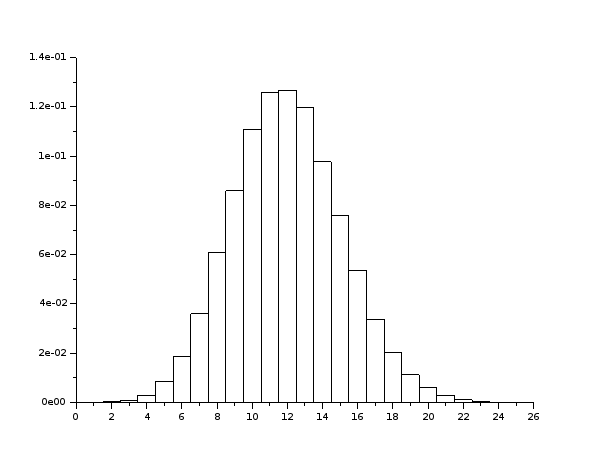
\includegraphics[scale=0.5]{Exo_incendie.png}
  \end{center}
  Que représente la valeur maximale prise par cet histogramme ?
  Prouver un résultat concernant cette valeur.
\end{exerciceSP}


\newpage


\begin{exerciceAP}~
  \begin{noliste}{1.}
    \setlength{\itemsep}{2mm}
  \item Question de cours : Soit $I$ un intervalle de $\R$ et $f$ une
    fonction continue sur $I$.\\
    Propriétés de l'application $x\in I \mapsto \dint{a}{x} f(t)\dt$.\\
    Soit $E$ l'espace vectoriel des fonctions continues sur $\R$ à
    valeurs réelles.\\
    Pour tout fonction $f\in E$, on note $T(f)$ l'application définie
    sur $\R$ à valeurs réelles, telle que :
    \[
    \forall x\in\R, \ T(f)(x)=\dint{x-1}{x+1} f(t)\dt.
    \]
  \item Pour tout $a\in\R$, soit $f_a$ la fonction définie sur $\R$
    par : $f_a(x)=\ee^{ax}$. Déterminer $T(f_a)$.
  \item 
    \begin{noliste}{a)}
    \setlength{\itemsep}{2mm}
    \item Montrer que pour toute fonction $f\in E$, l'application
      $T(f)$ appartient à $E$ et est de classe $\Cont 1$ sur $\R$.\\
      Déterminer la fonction dérivée de la fonction $T(f)$.
    \item On suppose que $f$ est une fonction bornée de $E$. Montrer
      que $T(f)$ est bornée et établir l'existence d'un réel $K$ tel
      que pour tout $(x,y)\in\R^2$, on a $\vert T(f)(x)-T(f)(y)\vert
      \leq K \vert x-y\vert$.
    \end{noliste}

  \item Soit $T$ l'application de $E$ dans $E$ qui à $f\in E$, associe
    $T(f)$.
    \begin{noliste}{a)}
    \setlength{\itemsep}{2mm}
    \item Montrer que $T$ est un endomorphisme de $E$. Est-il
      surjectif ?
    \item Soit $n\in\N$ et $\R_n[X]$ l'espace vectoriel des polynômes
      à coefficients réels de degré inférieur ou égal à $n$.\\
      Montrer que $T\left(\R_n[X]\right) \subset \R_n[X]$.
    \item Soit $T_n$ la restriction à $\R_n[X]$ de l'endomorphisme $T$
      et $\B=(1,X,X^2,\hdots, X^n)$ la base canonique de $\R_n[X]$.\\
      L'endomorphisme $T_n$ est-il diagonalisable ? $T_n$ est-il
      bijectif ?
    \end{noliste}
  \end{noliste}
\end{exerciceAP}


\begin{exerciceSP}~\\
  Soit $(X_n)_{n\in\N^*}$ une suite de variables aléatoires
  indépendantes définies sur un espace probabilisé $(\Omega,\A,P)$, de
  même loi de Bernoulli de paramètre $\dfrac{1}{2}$. On pose pour tout
  $n\in\N^*$ : $W_n=\Sum{k=1}{n} k X_k$.
  \begin{noliste}{1.}
    \setlength{\itemsep}{2mm}
  \item Calculer $\E(W_n)$ et $\V(W_n)$.
  \item Les variables $W_n$ et $W_{n+1}$ sont-elles indépendantes ?
  \end{noliste}
\end{exerciceSP}


\newpage


\begin{exerciceAP}~
  \begin{noliste}{1.}
    \setlength{\itemsep}{2mm}
  \item Question de cours : Définition d'un isomorphisme d'espaces vectoriels.\\
    Dans tout l'exercice, $n$ désigne un entier supérieur ou égal à
    $1$. Si $p\in\N$, on note $\R_p[X]$ l'ensemble des polynômes à
    coefficients réels de degré inférieur ou égal à $p$.\\
    On note $I_n$ la matrice identité de $\M{n}$. On rappelle que si
    $A\in\M{n}$ et $P(X) = \Sum{k=0}{p} a_kX^k$ un polynôme de
    $\R_p[X]$, alors $P(A)$ désigne la matrice $a_0 I_n+a_1 A+\cdots +
    a_p A^p$.

  \item Soit $A$ et $Q$ deux matrices de $\M{n}$. On suppose que la
    matrice $Q$ est inversible, d'inverse notée $Q^{-1}$.\\
    Soit $P$ un polynôme à coefficients réels. Expliciter
    $P(Q^{-1}AQ)$ en fonction de $P(A)$, $Q$ et $Q^{-1}$.

  \item 
    \begin{noliste}{a)}
    \setlength{\itemsep}{2mm}
    \item Soit $x_1,x_2,\hdots,x_n$ des réels deux à deux distincts et
      soit $\varphi$ l'application de $\R_{n-1}[X]$ dans $\R^n$ qui à
      tout polynôme $P\in\R_{n-1}[X]$, associe le $n$-uplet
      $\left(P(x_1), P(x_2), \hdots, P(x_n)\right)$. Montrer que
      l'application $\varphi$ est bijective.

    \item Soit $\lambda_1,\lambda_2,\hdots,\lambda_n$ $n$ réels
      distincts non nuls et $T=(t_{i,j})_{1\leq i,j\leq n}\in\M{n}$
      une matrice triangulaire telle que pour tout $i\in\llb 1,n\rrb$,
      $t_{i,i}=\lambda_i$.\\
      Établir l'existence d'un unique polynôme $P\in\R_{n-1}[X]$ tel
      que pour tout $i\in\llb 1,\rrb$, on a : $\lambda_i \times
      P(\lambda_i) = 1$.\\
      Que vaut $T \times P(T)$ ? Conclure.
    \end{noliste}
  \item Déterminer un polynôme $P\in\R_2[X]$ tel que $\forall
    (a,b,c)\in\R^3$, l'inverse de la matrice $A =
    \begin{smatrix}
      1 & a & b \\ 
      0 & 2 & c \\ 
      0 & 0 & 3
    \end{smatrix}$ soit égale à $P(A)$.
  \end{noliste}
\end{exerciceAP}


\begin{exerciceSP}~\\
  Soit $X_1,X_2,\hdots,X_n$ $n$ variables aléatoires telles que pour
  tout $k\in\llb 1,n\rrb$, $X_k$ suit la loi de Bernoulli de paramètre
  $p_k$ avec $0<p_k<1$.\\
  On pose : $Y=\Sum{k=1}{n} X_k$. Montrer que $\V(Y)\leq
  \dfrac{n^2}{4}$.
\end{exerciceSP}


\newpage


\begin{exerciceAP}~
  \begin{noliste}{1.}
    \setlength{\itemsep}{2mm}
  \item Question de cours : Formule des probabilités totales.\\
    Soit $n$ un entier naturel supérieur ou égal à $2$.\\
    On considère $n$ urnes numérotées de $1$ à $n$ et $N$ un entier
    naturel multiple de $2^n$.\\
    Pour tout $k\in\llb 1,n\rrb$, la $k$-ième urne contient $N$ boules
    dont $\dfrac{N}{2^k}$ boules blanches, les autres étant noires.\\
    On tire dans l'urne $1$ une boule au l'on place dans l'urne $2$,
    puis on tire dans l'urne $2$ une boule que l'on place dans l'urne
    $3$ et ainsi de suite jusqu'à tirer dans l'urne $n-1$ une boule
    que l'on place dans l'urne $n$, puis on tire une boule dans l'urne
    $n$.\\
    L'expérience est modélisée par un espace probabilisé
    $(\Omega,\A,P)$.
  \item Pour tout $k\in\llb 1,n\rrb$, soit $p_k$ la probabilité que la
    boule tirée dans l'urne $k$ soit blanche.\\
    Trouver une relation de récurrence entre $p_{k+1}$ et $p_k$
    ($1\leq k\leq n-1$).
  \item 
    \begin{noliste}{a)}
    \setlength{\itemsep}{2mm}
    \item Calculer $p_n$ en fonction de $n$ et $N$.
    \item Pour $n$ fixé, calculer $\dlim{N\to+\infty}
      p_n$. Interpréter cette limite.
    \end{noliste}
  \item Soit $i\in\llb 1,n-1\rrb$. Calculer la probabilité
    conditionnelle que la $n$-ième boule tirée soit blanche sachant
    que la boule tirée dans l'urne $i$ est blanche.
  \end{noliste}
\end{exerciceAP}


\begin{exerciceSP}~\\
  Soit $(u_n)_{n\in\N^*}$ la suite définie par : $\forall n\in\N^*$,
  $u_n=\dfrac{1}{n}\Sum{k=1}{n} \ln\left(\dfrac{k}{n}\right)$.
  \begin{noliste}{1.}
    \setlength{\itemsep}{2mm}
  \item Montrer que la suite $(u_n)_{n\in\N^*}$ est convergente et
    calculer sa limite.
  \item Quelle est la nature de la suite $(n!)^{\frac{1}{n}}$ ?
  \end{noliste}
\end{exerciceSP}


\newpage


\begin{exerciceAP}~
  \begin{noliste}{1.}
    \setlength{\itemsep}{2mm}
  \item Question de cours : Définition et propriétés de la fonction de
    répartition d'une variable aléatoire à densité.\\
    {\it Dans cet exercice, les variables aléatoires sont définies sur
      un espace probabilisé $(\Omega,\A,P)$, à valeurs dans $\R_+$ et
      admettent une densité.}\\
    Soit $X$ une variable aléatoire à densité admettant une espérance
    $\E(X)$. On note respectivement $F$ et $f$, la fonction de
    répartition et une densité de $X$.\\
    Soit $(X_n)_{n\in\N^*}$ une suite de variables aléatoires
    indépendantes de même loi que $X$.

  \item Pour $x\geq 0$ :
    \begin{noliste}{a)}
    \setlength{\itemsep}{2mm}
    \item Justifier la convergence de l'intégrale $\dint{x}{+\infty}
      tf(t)\dt$.

    \item Établir les inégalités : $\dint{x}{+\infty} tf(t) \dt \geq
      x(1-F(x))\geq 0$.

    \item Montrer à l'aide d'une intégration par parties que :
      $\E(X)=\dint{0}{+\infty} (1-F(t))\dt$.
    \end{noliste}

  \item Pour tout $n\in\N^*$, on note $Z_n=\max(X_1,X_2,\hdots,X_n)$,
    $G_n$ la fonction de répartition de $Z_n$ et $g_n$ une densité de
    $Z_n$.
    \begin{noliste}{a)}
    \setlength{\itemsep}{2mm}
    \item Exprimer pour tout $t\in\R$, $G_n(t)$ en fonction de $F(t)$.
    \item Établir l'existence de $\E(Z_n)$.
    \item Pour $n\geq 2$, montrer que : $\E(Z_n)-\E(Z_{n-1})=
      \dint{0}{+\infty} (F(t))^{n-1}(1-F(t))\dt$.
    \item Soit $m>0$. On suppose que $X$ suit la loi exponentielle de
      paramètre $m$ (d'espérance $\dfrac{1}{m}$). Calculer $\E(Z_n)$.\\
      Donner un équivalent de $\E(Z_n)$ lorsque $n$ tend vers
      $+\infty$.
    \end{noliste}
  \end{noliste}
\end{exerciceAP}


\begin{exerciceSP}~\\
  Soit $n$ un entier supérieur ou égal à $2$ et $X$ une matrice
  colonne non nulle de $\M{n,1}$.\\
  On pose : $A=X ^t X$.
  \begin{noliste}{1.}
    \setlength{\itemsep}{2mm}
  \item Montrer que $A$ est diagonalisable.
  \item Déterminer les valeurs propres et les sous-espaces propres de
    $A$.
  \end{noliste}
\end{exerciceSP}


\newpage


\begin{exerciceAP}~
  \begin{noliste}{1.}
    \setlength{\itemsep}{2mm}
  \item Question de cours : Donner des critères de convergence des
    séries à termes positifs.\\
    Soit $f$ la fonction définie sur $\R_+^*$ par $f(x)=\ln\left(
      \dfrac{\ee}{2}\left(x+\dfrac{1}{x}\right)\right)$.\\
    On note $(\Cont)$ la courbe représentative de $f$ dans le plan
    rapporté à un repère orthonormé.
  \item Dresser le tableau de variation de $f$.
  \item
    \begin{noliste}{a)}
    \setlength{\itemsep}{2mm}
    \item Montrer que la courbe $(\Gamma)$ d'équation
      $y=\ln\left(\dfrac{\ee}{2}x\right)$ est asymptote à $(\Cont)$.
    \item Tracer $(\Cont)$ et $(\Gamma)$ dans le même repère.
    \end{noliste}
  \item Établir pour tout réel $x\geq 1$, l'encadrement : $0\leq f'(x)<1$.\\
    En déduire que le signe de $f(x)-x$ pour tout $x\geq 1$ ainsi que
    la position de $(\Cont)$ par rapport à la droite $(\mathcal{D})$
    d'équation $y=x$.
  \item Soit le programme \Scilab{} suivant :
    \begin{scilab}
      & \tcFun{function} \tcVar{y}=f(\tcVar{x}) \nl %
      & \qquad \tcVar{y} = log(\%e \Sfois{} (\tcVar{x} + \tcVar{x}
      \puis (-1))/2) \nl %
      & \tcFun{endfunction} \nl %
      & \nl %
      & x = [0.01:0.1:5] ; \nl %
      & plot2d(x, f(x), rect=[0,0,5,5]) \nl %
      & \nl %
      & x = [0,5] \nl %
      & plot2d(x,x) \nl %
      & \nl %
      & u = input(\ttq{}u0=\ttq{}) \nl %
      & x = [u] ; y = [0] \nl %
      & \tcFor{for} k=1:10 \nl %
      & \qquad z = f(u) \nl %
      & \qquad x = [x,u] \nl %
      & \qquad x = [x,z] \nl %
      & \qquad y = [y,z,z] \nl %
      & \qquad u = z \nl %
      & \tcFor{end} \nl %
      & plot2d(x,y) \nl %
    \end{scilab}
    Expliquer ce que fait ce programme et ce qu'il illustre.\\
    Dans \texttt{plot2d}, \texttt{rect[0,0,5,5]} signifie que seule la
    partie de la courbe contenue dans le rectangle $\{(x,y)\ / \ 0\leq
    x\leq 5 \mbox{ et } 0\leq y \leq 5\}$ sera tracée.

  \item Étudier la suite $(u_n)_{n\in\N}$ définie par :
    $u_0\in[1,+\infty[$ et $\forall n\in\N$, $u_{n+1}=f(u_n)$.

  \item
    \begin{noliste}{a)}
    \setlength{\itemsep}{2mm}
    \item Justifier l'existence d'un réel $a>1$ tel que $x\in[1,a]
      \Rightarrow f'(x)\leq \dfrac{1}{2}$.
    \item On pose : $\forall n\in\N$, $v_n=u_n-1$. Quelle est la
      nature de la série de terme général $v_n$ ?
    \end{noliste}
  \end{noliste}
\end{exerciceAP}



\begin{exerciceSP}~\\
  Soit $(X_n)_{n\in\N^*}$ une suite de variables aléatoires telles que
  pour tout $n\geq 1$, $X_n$ admet une densité $f_n$ continue sur
  $\R$, nulle sur $\R_-$ et sur $\left[\dfrac{2}{n},+\infty\right[$,
  affine sur $\left[0,\dfrac{1}{n}\right]$ et sur
  $\left[\dfrac{1}{n},\dfrac{2}{n}\right]$.
  \begin{noliste}{1.}
    \setlength{\itemsep}{2mm}
  \item Déterminer une densité $f_n$ de $X_n$.
  \item Étudier la convergence en loi de la suite de variables
    aléatoires $(X_n)_{n\in\N^*}$.
  \end{noliste}
\end{exerciceSP}


\newpage


\begin{exerciceAP}~\\
  {\it Toutes les variables aléatoires de cet exercice sont définies
    sur un espace probabilisé $(\Omega,\A,P)$}.
  \begin{noliste}{1.}
    \setlength{\itemsep}{2mm}
  \item Question de cours : Définition et propriétés de la fonction de
    répartition d'une variable aléatoire à densité.\\
    Soit $a$ un paramètre réel et $F$ la fonction définie sur $\R$, à
    valeurs réelles, telle que :
    \[
    F(x)=\left\{
      \begin{array}{cl}
        1+\ln\left(\dfrac{x}{x+1}\right) & \mbox{ si $x\geq a$}\\
        0 & \mbox{ si $x<a$}
      \end{array}
    \right.
    \]
  \item 
    \begin{noliste}{a)}
    \setlength{\itemsep}{2mm}
    \item Montrer que $F$ est continue sur $\R$ si et seulement si
      $a=\dfrac{1}{\ee -1}$.

    \item Étudier les variations de $F$ et tracer l'allure de sa
      courbe représentative dans un repère orthogonal du plan.
    \end{noliste}

  \item
    \begin{noliste}{a)}
    \setlength{\itemsep}{2mm}
    \item Montrer que $F$ est la fonction de répartition d'une
      variable aléatoire $X$ à densité.
    \item La variable aléatoire $X$ admet-elle une espérance ?
    \end{noliste}

  \item Soit $Y$ la variable aléatoire à valeurs dans $\N$ définie par
    $Y=\lfloor X\rfloor$ (partie entière de $X$). On pose : $Z=X-Y$.
    \begin{noliste}{a)}
    \setlength{\itemsep}{2mm}
    \item Calculer $\Prob(Y=0)$ et montrer que pour tout $n\in\N^*$, on a
      : $\Prob(Y=n)=\ln\left(1+\dfrac{1}{n(n+2)}\right)$.
    \item Déterminer la fonction de répartition et une densité de $Z$.
    \item Établir l'existence de l'espérance $\E(Z)$ de $Z$. Calculer
      $\E(Z)$.
    \end{noliste}
  \end{noliste}
\end{exerciceAP}


\begin{exerciceSP}~\\
  Soit $a$, $b$ et $c$ des réels non nuls vérifiant
  $a^2+b^2+c^2 = 1$. On pose : $U = 
  \begin{smatrix} 
    a\\ 
    b\\
    c
  \end{smatrix} \in \M{3,1}$.
  \begin{noliste}{1.}
    \setlength{\itemsep}{2mm}
  \item 
    \begin{noliste}{a)}
    \setlength{\itemsep}{2mm}
    \item Calculer la matrice $M=U ^t U$ (où $^t U$ est la matrice
      transposée de la matrice colonne $U$).
    \item $M$ est-elle diagonalisable ? inversible ?
    \end{noliste}
  \item
    \begin{noliste}{a)}
    \setlength{\itemsep}{2mm}
    \item Pour $n\in\N^*$, calculer $M^n$.
    \item Quelles sont les valeurs propres de $M$ et les sous-espaces
      propres associés.
    \end{noliste}
  \end{noliste}
\end{exerciceSP}


\newpage


\section{Annales 2014}

%\setcounter{exercice}{0}

\begin{exerciceAP}~
  \begin{noliste}{1.}
    \setlength{\itemsep}{2mm}
  \item Question de cours : Définition de l'indépendance de deux
    variables aléatoires discrètes. Lien entre indépendance et
    covariance.\\
    Soit $X$ et $Y$ deux variables aléatoires discrètes finies à
    valeurs dans $\N$, définies sur un espace probabilisé
    $(\Omega,\A,P)$. On suppose que $X(\Omega)\subset \llb0,n\rrb$ et
    $Y(\Omega)\subset \llb0,m\rrb$, où $n$ et $m$ sont deux entiers de
    $\N^*$.\\
    Pour tout couple $(i,j)\in\llb0,n\rrb\times\llb0,m\rrb$, on pose :
    $p_{i,j}=\Prob(\Ev{X=i}\cap\Ev{Y=j})$.\\
    Soit $F_X$ et $F_Y$ les deux fonctions de $\R$ dans $\R$ définies
    par : $F_X(x)=\Sum{i=0}{n} \Prob(\Ev{X=i})x^i$ et \\
    $F_Y(x)=\Sum{j=0}{m} \Prob(\Ev{Y=j})x^j$.\\
    Soit $Z=(X,Y)$ et $G_Z$ la fonction de $\R^2$ dans $\R$ définie
    par : $G_Z(x,y)=\Sum{i=0}{n}\Sum{j=0}{m} p_{i,j}x^iy^j$.

  \item Donner la valeur de $G_Z(1,1)$ et exprimer les espérances de
    $X$, $Y$ et $XY$, puis la covariance de $(X,Y)$ à l'aide des
    dérivées partielles premières et secondes de $G_Z$ au point
    $(1,1)$.

  \item Soit $f$ une fonction polynomiale de deux variables définies
    sur $\R^2$ par : $f(x,y)=\Sum{i=0}{n}\Sum{j=0}{m} a_{i,j}x^iy^j$
    avec $a_{i,j}\in\R$.\\
    On suppose que pour tout couple $(x,y)\in\R^2$, on a $f(x,y)=0$.
    \begin{noliste}{a)}
    \setlength{\itemsep}{2mm}
    \item Montrer que pour tout
      $(i,j)\in\llb0,n\rrb\times\llb0,m\rrb$, on a $a_{i,j}=0$.
    \item En déduire que $X$ et $Y$ sont indépendantes, si et
      seulement si, pour tout $(x,y)\in\R^2$,\\
      $G_Z(x,y)=F_X(x)F_Y(y)$. (on pourra poser : $a_{i,j}=p_{i,j} -
      \Prob(\Ev{X=i})\Prob(\Ev{Y=j})$).
    \end{noliste}

  \item Une urne contient des jetons portant chacun une des lettres
    $A$, $B$ ou $C$. La proportion des jetons portant la lettre $A$
    est $p$, celle des jetons portant la lettre $B$ est $q$ et celle
    des jetons portant la lettre $C$ est $r$, où $p$, $q$ et $r$ sont
    trois réels strictement positifs vérifiant $p+q+r=1$.\\
    Soit $n\in\N^*$. On effectue $n$ tirages d'un jeton avec remise
    dans cette urne. On note $X$ (resp. $Y$) la variable aléatoire
    égale au nombre de jetons tirés portant la lettre $A$ (resp. $B$)
    à l'issue de ces $n$ tirages.
    \begin{noliste}{a)}
    \setlength{\itemsep}{2mm}
    \item Quelles sont les lois de $X$ et $Y$ respectivement ?
      Déterminer $F_X$ et $F_Y$.
    \item Déterminer la loi de $Z$. En déduire $G_Z$.
    \item Les variables aléatoires $X$ et $Y$ sont-elles indépendantes
      ?
    \item Calculer la covariance de $(X,Y)$. Le signe de cette
      covariance était-il prévisible ?
    \end{noliste}
  \end{noliste}
\end{exerciceAP}


\begin{exerciceSP}~\\
  Soit $n\in\N^*$ et $A$ une matrice de $\M{n}$ telle que $A ^t AA ^t
  AA=I$, où $I$ est la matrice identité de $\M{n}$.
  \begin{noliste}{1.}
    \setlength{\itemsep}{2mm}
  \item Montrer que la matrice $A$ est symétrique.
  \item Déterminer $A$.
  \end{noliste}
\end{exerciceSP}



\newpage


\begin{exerciceAP}~
  \begin{noliste}{1.}
    \setlength{\itemsep}{2mm}
  \item Question de cours : Définition et représentation graphique de
    la fonction partie entière.\\
    On note $E$ l'espace vectoriel des applications de $\R$ dans $\R$
    et $F$ le sous-espace vectoriel de $E$ engendré par les quatre
    fonctions $f_0$, $f_1$, $f_2$ et $f_3$ définies par :
    \[
    \forall x\in\R, \ f_0(x)=1, \ f_1(x)=x, \ f_2(x)=\ee^x, \
    f_3(x)=x\ee^x.
    \]

  \item On note : $\B=(f_0,f_1,f_2,f_3)$.
    \begin{noliste}{a)}
    \setlength{\itemsep}{2mm}
    \item Montrer que $\B$ est une base de $F$.
    \item Montrer que toutes les fonctions de $F$ sont continues et
      dérivables sur $\R$.
    \end{noliste}

  \item Soit $\Phi$ l'application définie par : pour tout $f\in F$,
    $\Phi(f)=f'$, où $f'$ est la dérivée de $f$.
    \begin{noliste}{a)}
    \setlength{\itemsep}{2mm}
    \item Justifier que $\Phi$ est un endomorphisme de $F$ et écrire
      la matrice $M$ de $\Phi$ dans la base $\B$.
    \item L'endomorphisme $\Phi$ est-il diagonalisable ?
    \item Montrer que $f_3$ appartient à $\im(\Phi)$ et résoudre dans
      $F$ l'équation : $\Phi(f)=f_3$.
    \end{noliste}

  \item On note $G$ l'ensemble des fonctions $g$ de $E$ telles que :
    \[
    \forall x\in\R, \ g(x+1)-g(x)=0.
    \]
    \begin{noliste}{a)}
    \setlength{\itemsep}{2mm}
    \item Montrer que $G$ est un sous-espace vectoriel de $E$ et
      trouver $F\cap G$.
    \item Trouver un élément de $G$ qui n'appartienne pas à $F$.
    \end{noliste}
  \item Trouver toutes les fonctions de $F$ vérifiant : $\forall
    x\in\R$, $f(x+1-f(x)=(\ee -1)f'(x)$.
  \end{noliste}
\end{exerciceAP}


\begin{exerciceSP}~\\
  Soit $p$ un réel de $]0,1[$ et $q=1-p$. Soit $(X_n)_{n\in\N^*}$ une
  suite de variables aléatoires indépendantes définies sur un espace
  probabilisé $(\Omega,\A,P)$, de même loi de Bernoulli telle que :\\
  $\forall k\in\N^*$, $\Prob(\Ev{X_k=1}) = p$ et $\Prob(\Ev{X_k=0}) =
  q$. Pour $n$ entier de $\N^*$, on définit pour tout
  $k\in\llb1,n\rrb$ la variable aléatoire $Y_k=X_k+X_{k+1}$.
  \begin{noliste}{1.}
    \setlength{\itemsep}{2mm}
  \item 
    \begin{noliste}{a)}
    \setlength{\itemsep}{2mm}
    \item Calculer pour tout $k\in\llb1,n\rrb$, $\Cov(Y_k,Y_{k+1})$.
    \item Montrer que $0<\Cov(Y_k,Y_{k+1})\leq \dfrac{1}{4}$.
    \end{noliste}
  \item Calculer pour tout couple $(k,l)$ tel que $1\leq k<l\leq n$,
    $\Cov(Y_k,Y_l)$.
  \item On note $\eps$ un réel strictement positif fixé. Montrer que
    $\dlim{n\to+\infty} \Prob \left(\Ev{\left \vert
          \dfrac{1}{n}\Sum{k=1}{n} Y_k -2p \right\vert >\eps}\right)
    =0$.
  \end{noliste}
\end{exerciceSP}


\newpage


\begin{exerciceAP}~
  \begin{noliste}{1.}
    \setlength{\itemsep}{2mm}
  \item Question de cours : Définition de deux matrices semblables.\\
    Soit $E$ un espace vectoriel sur $\R$ de dimension $2$. On note
    $\LL{E}$ l'ensemble des endomorphismes de $E$.\\
    Pour toute matrice $A=\begin{smatrix} a & c\\ b & d\end{smatrix}
    \in\M{2}$, on note $D$ et $T$ les deux applications suivantes :
    \[
    D:\left\{
      \begin{array}{rcl}
        \M{2} & \rightarrow & \R\\
        A & \mapsto & ad-bc
      \end{array}
    \right. \quad \mbox{et} \quad T:\left\{
      \begin{array}{rcl}
        \M{2} & \rightarrow & \R\\
        A & \mapsto & a+d
      \end{array}
    \right.
    \]

  \item Soit $A$ et $B$ deux matrices de $\M{2}$.
    \begin{noliste}{a)}
    \setlength{\itemsep}{2mm}
    \item Exprimer $D(AB)$ en fonction de $D(A)$ et $D(B)$. Montrer
      que $T(AB)=T(BA)$.
    \item En déduire que si $A$ et $B$ sont semblables, on a
      $D(A)=D(B)$ et $T(A)=T(B)$.
    \end{noliste}

  \item Déterminer $\ker(D)$ et $\ker(T)$. Quelle est la dimension de
    $\ker(T)$ ?\\
    Dorénavant, si $u\in\ll{E}$ de matrice $A$ dans une base $\B$ de
    $E$, on note : $D(u)=D(A)$ et $T(u)=T(A)$.

  \item On note $\id_E$ l'endomorphisme identité de $E$. Exprimer
    $u^2=u\circ u$ en fonction de $u$ et $\id_E$.

  \item Soit $u\in\LL{E}$ et $\mathcal{S}_0=\{v\in\LL{E} \vert u \circ
    v-v\circ u=0\}$.\\
    Montrer que $\mathcal{S}_0$ est un espace vectoriel contenant
    $\{P(u),P\in\R[X]\}$.

  \item Soit $u\in\LL{E}$ avec $u\neq 0$. On pose :
    $\mathcal{S}=\{v\in\LL{E} \vert u\circ v -v\circ u =u\}$.
    \begin{noliste}{a)}
    \setlength{\itemsep}{2mm}
    \item Montrer que si $\mathcal{S}$ est non vide, alors
      l'endomorphisme $u$ ne peut être bijectif. En déduire une
      condition nécessaire et suffisante portant sur $u^2$ pour que
      $\mathcal{S}$ soit non vide.
    \item On suppose que $\mathcal{S}$ est non vide. Établir
      l'existence d'une base $\B_1=(e_1,e_2)$ de $E$ dans laquelle la
      matrice $M_u$ de $u$ d'écrit $M_u = 
      \begin{smatrix} 
        0 & 1\\ 
        0 & 0
      \end{smatrix}$ et déterminer la forme générale de la matrice des
      éléments $v$ de $\mathcal{S}$ dans cette même base.
    \item On suppose que $\mathcal{S}$ est non vide. Montrer que
      $\mathcal{S}=\{v_0+\alpha \id_E+\beta u, \alpha, \beta\in\R\}$
      où $v_0$ est un endomorphisme non inversible de $E$ à
      déterminer.
    \end{noliste}
  \end{noliste}
\end{exerciceAP}


\begin{exerciceSP}~\\
  Soit $k$ et $\lambda$ deux réels et soir $f$ la fonction définie sur
  $\R$ à valeurs réelles donnée par :
  \[
  f(t)=\left\{
    \begin{array}{cl}
      kt\ee^{-\lambda t} & \mbox{ si $t\geq 0$}\\
      0 & \mbox{ sinon}
    \end{array}
  \right.
  \]
  \begin{noliste}{1.}
    \setlength{\itemsep}{2mm}
  \item Exprimer $k$ en fonction de $\lambda$ pour que $f$ soit une
    densité de probabilité.\\
    On note $X$ une variable aléatoire réelle ayant $f$ pour densité.
  \item Montrer que pour tout $n\in\N^*$, la variable aléatoire $X$
    admet un moment d'ordre $n$ que l'on calculera.
  \end{noliste}
\end{exerciceSP}


\newpage


\begin{exerciceAP}~
  \begin{noliste}{1.}
    \setlength{\itemsep}{2mm}
  \item Question de cours : Loi d'un couple de variables aléatoires
    discrètes. Lois marginales. Lois conditionnelles.\\
    Soit $c$ un réel strictement positif et soit $X$ et $Y$ deux
    variables aléatoires à valeurs dans $\N$ définies sur un espace
    probabilisé $(\Omega,\A,P)$, telles que :
    \[
    \forall (i,j)\in\N^2, \ \Prob(\Ev{X=i}\cap\Ev{Y=j}) =
    c\dfrac{i+j}{i!j!}.
    \]
  \item 
    \begin{noliste}{a)}
    \setlength{\itemsep}{2mm}
    \item Montrer que pour tout $i\in\N$, on a :
      $\Prob(\Ev{X=i})=c\dfrac{(i+1)}{i!}\ee$. En déduire la valeur de
      $c$.
    \item Montrer que $X$ admet une espérance et une variance et les
      calculer.
    \item Les variables aléatoires $X$ et $Y$ sont-elles indépendantes
      ?
    \end{noliste}
  \item
    \begin{noliste}{a)}
    \setlength{\itemsep}{2mm}
    \item Déterminer la loi de $X+Y-1$.
    \item En déduire la variance de $X+Y$.
    \item Calculer la covariance de $X$ et de $X+5Y$. Les variables
      aléatoires $X$ et $X+5Y$ sont-elles indépendantes ?
    \end{noliste}

  \item On pose : $Z=\dfrac{1}{X+1}$.
    \begin{noliste}{a)}
    \setlength{\itemsep}{2mm}
    \item Montrer que $Z$ admet une espérance et la calculer.
    \item Déterminer pour $i\in\N$, la loi conditionnelle de $Y$
      sachant $\Ev{X=i}$.
    \item Pour $A\in\A$, on pose : $g_A(Y)=\Sum{k=0}{+\infty} k
      P_A(\Ev{Y=k})$.\\
      Établir l'existence d'une fonction affine $f$ telle que, pour
      tout $\omega\in\Omega$, on a : $g_{\Ev{X=X(\omega)}}(Y) =
      f(Z(\omega))$.
    \end{noliste}
  \end{noliste}
\end{exerciceAP}


\begin{exerciceSP}~
  \begin{noliste}{1.}
    \setlength{\itemsep}{2mm}
  \item La somme de deux matrices diagonalisables est-elle
    diagonalisable ?
  \item La somme de deux matrices inversibles est-elle inversible ?
  \item Montrer que toute matrice carrée est la somme de deux matrices
    inversibles?
  \end{noliste}
\end{exerciceSP}


\newpage


\begin{exerciceAP}~\\
  On note $\M{3}$ l'ensemble des matrices carrées d'ordre $3$ et
  $\R_2[X]$ l'ensemble des polynômes à coefficients réels de degré
  inférieur ou égal à $2$.\\
  Dans tout l'exercice, $A$ est une matrice de $\M{3}$ ayant trois
  valeurs propres distinctes, notées $\lambda_1$, $\lambda_2$ et
  $\lambda_3$.
  \begin{noliste}{1.}
    \setlength{\itemsep}{2mm}
  \item Question de cours :Définition d'un polynôme annulateur d'une
    matrice. Lien avec les valeurs propres.
  \item
    \begin{noliste}{a)}
    \setlength{\itemsep}{2mm}
    \item Donner en fonction de $\lambda_1$, $\lambda_2$ et
      $\lambda_3$, un polynôme annulateur de $A$ de degré $3$.
    \item Peut-on trouver un polynôme annulateur de $A$ de degré $1$
      ou de degré $2$ ?
    \end{noliste}

  \item Soit $\varphi$ l'application de $\R_2[X]$ dans $\R^3$ qui à
    tout polynôme $P\in\R_2[X]$, associe le triplet
    $\left(P(\lambda_1^5),P(\lambda_2^5), P(\lambda_3^5)\right)$.
    \begin{noliste}{a)}
    \setlength{\itemsep}{2mm}
    \item Montrer que l'application $\varphi$ est linéaire.
    \item Déterminer $\ker(\varphi)$.
    \item L'application $\varphi$ est-elle un isomorphisme de
      $\R_2[X]$ sur $\R^3$ ?
    \item Établir l'existence d'un unique polynôme $Q\in\R_2[X]$ tel
      que : pour tout $i\in\llb1,3\rrb$, $Q(\lambda_i^5)=\lambda_i$.
    \item Soit $T$ le polynôme défini par : $T(X)=Q(X^5)-X$.\\
      Montrer que le polynôme $T$ est un polynôme annulateur de $A$.
    \end{noliste}

  \item On note $\mathcal{E}$ et $\mathcal{F}$ les deux sous-ensembles
    de $\M{3}$ suivants :
    \[
    \mathcal{E}=\{N\in\M{3} \setminus AN=NA\} \ \mbox{ et } \
    \mathcal{F}=\{N\in\M{3} \setminus A^5N=NA^5\}.
    \]
    Déduire des questions précédentes que $\mathcal{E}=\mathcal{F}$.
  \end{noliste}
\end{exerciceAP}


\begin{exerciceSP}~\\
  Soit $(X_n)_{n\in\N^*}$ une suite de variables aléatoires définies
  sur un espace probabilisé $(\Omega,\A,P)$, indépendantes et de même
  loi exponentielle de paramètre $\lambda>0$.\\
  Pour $n\in\N^*$, on pose : $M_n=\max(X_1,\hdots,X_n)$ et on admet
  que $M_n$ est une variable aléatoire définie sur $(\Omega,\A,P)$.
  \begin{noliste}{1.}
    \setlength{\itemsep}{2mm}
  \item Déterminer la loi de $M_n$.
  \item Montrer que l'application $g$ qui à tout réel $x$ associe
    $g(x)=\ee^{-x}\exp\left(-\ee^{-x}\right)$ est une densité de
    probabilité.
  \item Soit $Y$ une variable aléatoire définie sur $(\Omega,\A,P)$ de
    densité $g$.\\
    Montrer que la suite de variables aléatoires $(\lambda M_n -
    \ln(n))_{n\geq 1}$ converge en loi vers $Y$.
  \end{noliste}
\end{exerciceSP}



\newpage


\begin{exerciceAP}~
  \begin{noliste}{1.}
    \setlength{\itemsep}{2mm}
  \item Question de cours : Définition de la convergence d'une série
    numérique (à termes réels).\\
    {\it Dans tout l'exercice, $a$ est un réel strictement supérieur à
      $1$.}
  \item
    \begin{noliste}{a)}
    \setlength{\itemsep}{2mm}
    \item Montrer que pour tout $n\in\N^*$, l'intégrale
      $\dint{0}{+\infty} \dfrac{dt}{(1+t^a)^n}$ est convergente. On
      pose alors pour tout $n\in\N^*$ : $u_n(a)=\dint{0}{+\infty}
      \dfrac{dt}{(1+t^a)^n}$.
    \item Établir la convergence de la suite $(u_n(a))_{n\in\N^*}$.
    \end{noliste}

  \item
    \begin{noliste}{a)}
    \setlength{\itemsep}{2mm}
    \item Montrer que pour tout $n\in\N^*$, on a :
      $u_n(a)=an(u_n(a)-u_{n+1}(a))$. En déduire $u_n(a)$ en fonction
      de $u_1(a)$.
    \item Montrer que la série de terme général
      $\left(\dfrac{u_n(a)}{an}\right)$ est convergente.
    \item En déduire la limite de la suite $(u_n(a))_{n\in\N^*}$.
    \end{noliste}

  \item On pose pour tout $n\in\N^*$ :
    $w_n(a)=\ln(u_n(a))+\dfrac{\ln(n)}{a}$.
    \begin{noliste}{a)}
    \setlength{\itemsep}{2mm}
    \item Montrer que la série de terme général $(w_{n+1}(a)-w_n(a))$
      est convergente.
    \item En déduire l'existence d'un réel $K(a)$ tel que $u_n(a)$
      soit équivalent à $\dfrac{K(a)}{n^{\frac{1}{a}}}$ lorsque $n$
      tend vers $+\infty$.
    \end{noliste}
  \end{noliste}
\end{exerciceAP}


\begin{exerciceSP}~\\
  Les variables aléatoires sont définies sur un espace probabilisé
  $(\Omega,\A,P)$.\\
  Soit $X$ une variable aléatoire qui suit la loi de Poisson de
  paramètre $\lambda>0$ et soit $Y$ une variable aléatoire
  indépendante de $X$ telle que : $Y(\Omega)=\{1,2\}$,
  $\Prob(\Ev{Y=1})=\Prob(\Ev{Y=2})=\dfrac{1}{2}$.\\
  On pose : $Z=XY$.
  \begin{noliste}{1.}
    \setlength{\itemsep}{2mm}
  \item Déterminer la loi de $Z$.
  \item On admet que : $\Sum{k=0}{+\infty}
    \dfrac{\lambda^{2k}}{(2k)!}=\dfrac{\ee^{\lambda}+\ee^{-\lambda}}{2}$. Quelle
    est la probabilité que $Z$ prenne des valeurs paires ?
  \end{noliste}
\end{exerciceSP}


\newpage


\begin{exerciceAP}~
  \begin{noliste}{1.}
    \setlength{\itemsep}{2mm}
  \item Question de cours : Critères de convergence d'une intégrale
    impropre.\\
    Préciser la nature de l'intégrale $\dint{a}{+\infty}
    \dfrac{dt}{t^\alpha}$, où $a$ est un réel strictement positif et
    $\alpha$ un réel quelconque.\\
    Soit $T$ une variable aléatoire d"finie sur un espace probabilisé
    $(\Omega,\A,P)$, suivnt la loi normale centrée réduite.\\
    On note $\Phi$ et $\varphi$ respectivement, la fonction de
    répartition et une densité de $T$.
  \item
    \begin{noliste}{a)}
    \setlength{\itemsep}{2mm}
    \item \`A l'aide de l'inégalité de Bienaymé-Tchebychev, montrer
      que pour tout $x>0$, on a :\\ $0\leq 1-\Phi(x)\leq
      \dfrac{1}{2x^2}$.
    \item En déduire que l'intégrale $\dint{0}{+\infty}
      (1-\Phi(x))\dx$ est convergente et calculer sa valeur.
    \end{noliste}

  \item On note $\varphi'$ la dérivée de $\varphi$.
    \begin{noliste}{a)}
    \setlength{\itemsep}{2mm}
    \item Déterminer pour tout $x\in\R$, une relation entre
      $\varphi'(x)$ et $\varphi(x)$.
    \item En déduire, à l'aide de deux intégrations par parties, que
      pour tout $x\in\R_+^*$, on a :\\
      $\dfrac{1}{x}-\dfrac{1}{x^3}\leq
      \dfrac{1-\Phi(x)}{\varphi(x)}\leq \dfrac{1}{x}$.
    \item Donner un équivalent de $1-\Phi(x)$ quand $x$ tend vers
      $+\infty$.
    \end{noliste}

  \item Soit $a>0$. Calculer $\dlim{x\to+\infty} \left(
      P_{\Ev{T>x}}\left[T>x+\dfrac{a}{x}\right]\right)$.
  \end{noliste}
\end{exerciceAP}


\begin{exerciceSP}~\\
  Soit $D$ la matrice définie par : $D = 
  \begin{smatrix} 
    -1 & 0\\ 
    0 & 4
  \end{smatrix}$.
  \begin{noliste}{1.}
    \setlength{\itemsep}{2mm}
  \item Déterminer les matrices $A\in\M{2}$ telles que $AD=DA$.
  \item En déduire les matrices $M\in\M{2}$ qui vérifient $M^3-2M=D$.
  \end{noliste}
\end{exerciceSP}


\newpage


\begin{exerciceAP}~
  \begin{noliste}{1.}
    \setlength{\itemsep}{2mm}
  \item Question de cours : Définition de deux matrices semblables.\\
    Soit $f$ un endomorphisme de $\R^3$ dont la matrice $A$ dans la
    base canonique de $\R^3$ est donnée par :
    \[
    A = 
    \begin{smatrix} 
      3 & 2 & -2\\ 
      -1 & 0 & 1\\ 
      1 & 1 & 0
    \end{smatrix}.
    \]
    On note $\id$ l'endomorphisme identité de $\R^3$ et on pose :
    $f^2=f\circ f$.
  \item
    \begin{noliste}{a)}
    \setlength{\itemsep}{2mm}
    \item Montrer que $2f-f^2=\id$.
    \item Montrer que l'endomorphisme $f$ est un automorphisme. Quel
      est l'automorphisme réciproque de $f$ ?
    \item Montrer que $f$ admet l'unique valeur propre
      $1$. L'endomorphisme $f$ est-il diagonalisable ?
    \item Déterminer le sous-espace propre associé à la valeur propre
      $1$. Quelle est sa dimension ?
    \end{noliste}

  \item
    \begin{noliste}{a)}
    \setlength{\itemsep}{2mm}
    \item Calculer pour tout $n\in\N$, $A^n$ en fonction de $n$.
    \item Le résultat précédent s'étend-t-il au cas où $n\in\Z$ ?
    \end{noliste}

  \item Déterminer une base $(u,v,w)$ de $\R^3$ dans laquelle la
    matrice de $f$ est la matrice $C = 
    \begin{smatrix} 
      1 & 0 & 0\\
      0 & 1 & 1\\ 
      0 & 0 & 1
    \end{smatrix}$.
  \end{noliste}
\end{exerciceAP}


\begin{exerciceSP}~
  Soit $(X_n)_{n\in\N^*}$ une suite de variables aléatoires
  indépendantes définies sur le même espace probabilisé
  $(\Omega,\A,P)$ et suivant toutes la loi uniforme sur l'intervalle
  $[0,1]$.
  \begin{noliste}{1.}
    \setlength{\itemsep}{2mm}
  \item Pour tout entier $k\geq 1$, déterminer une densité de la
    variable aléatoire $Y_k=\max(X_1,X_2,\hdots,X_k)$.
  \item Déterminer une densité de la variable aléatoire $Z_k=-Y_k$.
  \end{noliste}
\end{exerciceSP}


\newpage


\begin{exerciceAP}~\\
  \begin{noliste}{1.}
    \setlength{\itemsep}{2mm}
  \item Question de cours : Énoncer une condition nécessaire et
    suffisante de diagonalisabilité d'un endomorphisme.\\
    On considère la matrice $A\in\M{2}$ définie par $A=\begin{smatrix} 2 & 4\\
    1 & 2\end{smatrix}$.
  \item On note $\M{2,1}$ l'espace vectoriel des matrices à $2$ lignes
    et $1$ colonne à coefficients réels.\\
    Soit $u$ l'endomorphisme de $\M{2,1}$ défini par : pour tout
    $X\in\M{2,1}$, $u(X)=AX$.
    \begin{noliste}{a)}
    \setlength{\itemsep}{2mm}
    \item Déterminer une base de $\ker(u)$ et une base de $\im(u)$.
    \item L'endomorphisme $u$ est-il diagonalisable ?
    \item Calculer pour tout $n\in\N^*$, la matrice $A^n$.
    \end{noliste}

  \item Soit $v$ l'endomorphisme de $\M{2}$ défini par : pour tout
    $M\in\M{2}$, $v(M)=AM$.\\
    On note $\B=\left(E_{1,1},E_{1,2},E_{2,1},E_{2,2}\right)$ la base
    canonique de $\M{2}$ et on rappelle que :
    \[
    E_{1,1} = 
    \begin{smatrix} 
      1 & 0\\ 
      0 & 0
    \end{smatrix}, %
    \ E_{1,2} = 
    \begin{smatrix} 
      0 & 1 \\
      0 & 0 
    \end{smatrix}, %
    \ E_{2,1} = 
    \begin{smatrix} 
      0 & 0 \\ 
      1 & 0 
    \end{smatrix}, %
    \ E_{2,2} = 
    \begin{smatrix} 
      0 & 0 \\
      0 & 1
    \end{smatrix}
    \]
    \begin{noliste}{a)}
    \setlength{\itemsep}{2mm}
    \item Écrire la matrice $V$ de l'endomorphisme $v$ dans la base
      $\B$.
    \item Déterminer une base de $\ker(v)$ et une base de $\im(v)$.
    \item L'endomorphisme $v$ est-il diagonalisable ?
    \end{noliste}
\end{noliste}
\end{exerciceAP}


\begin{exerciceSP}~
  Soit $n$ un entier supérieur ou égal à $2$. On dispose de $n$ urnes
  $U_1$, $U_2$, $\hdots$, $U_n$ contenant chacune trois boules. Dans
  l'ensemble des $3n$ boules, une seule est rouge, les autres étant
  bleues.\\
  Sachant que l'on a tiré sans remise deux boules bleues dans l'urne
  $U_1$, quelle est la probabilité que l'urne $U_2$ contienne la boule
  rouge ?
\end{exerciceSP}


\newpage


\section{Annales 2013}

%\setcounter{exercice}{0}
\begin{exerciceAP}~\\
  \begin{noliste}{1.}
    \setlength{\itemsep}{2mm}
  \item Question de cours : Le schéma binomial.
  \item Soit $(X_n)_{ n \in \N^* }$ une suite de variables
    aléatoires définies sur un espace probabilisé $(\Omega , \A
    , P )$, indépendantes et de même loi de Bernoulli de paramètre
    $\frac{1}{2}$.\\
    
    On pose, pour tout $n \in \N^*$, $W_n = \Sum{k=1}{n} k
    X_k$ et $s_n = \frac{ n ( n+1 ) }{ 2 }$.

    \begin{noliste}{a)}
    \setlength{\itemsep}{2mm}

    \item Calculer l'espérance $E ( W_n )$ et la variance $V ( W_n )$ de
      la variable aléatoire $W_n$.

    \item Calculer les probabilités $\Prob( W_n = 0)$ et $P ( W_n = s_n)$.

    \item Calculer, selon les valeurs de $n$, la probabilité $P ( W_n = 3 )$.

    \end{noliste}

  \item Montrer que pour tout $k \in \llb 0 ; s_n \rrb$, on a : $\Prob(
    W_n = k ) = P ( W_n = s_n - k )$.

  \item 
    \begin{noliste}{a)}
    \setlength{\itemsep}{2mm}
    \item Déterminer pour tout $j \in \llb 0 ; s_n \rrb$ la loi de
      probabilité conditionnelle de $W_{n+1}$ sachant $(W_n = j)$.
    \item En déduire les relations :
      \[
      P ( W_{n+1} = k ) = \left\{ 
        \begin{array}{ll} 
          \frac{ 1 }{ 2 } P ( W_n = k ) & \text{ si } k \leq n \\ 
          \\ 
          \frac{ 1 }{ 2 } P (W_n = k) + \frac{ 1 }{ 2 }
          P ( W_n = k-n-1) & \text{ si } n+1 \leq k \leq s_n \\ 
          \\
          \frac{ 1 }{ 2 } P ( W_n = k-n-1) & \text{ si } s_n + 1 \leq
          k \leq s_{n+1} 
        \end{array} 
      \right.
      \]
    \end{noliste}
  \end{noliste}
\end{exerciceAP}


\begin{exerciceSP}~
  On pose pour tout $n \in \N^*$ : $S_n = \Sum{k=1}{n} k^2
  \ln \left( \frac{ k }{ n } \right)$.
  \begin{noliste}{1.}
    \setlength{\itemsep}{2mm}
  \item Déterminer $\dlim{n \rightarrow + \infty} \dfrac{S_n}{ n^3}$.

  \item En déduire la limite lorsque $n$ tend vers $+\infty$ de
    $\frac{1}{n^3} \Sum{k=1}{n} k^2 \ln \left( \frac{ k+1 }{ n }
    \right)$.

  \end{noliste}
\end{exerciceSP}


\newpage


\begin{exerciceAP}~\\
  \begin{noliste}{1.}
    \setlength{\itemsep}{2mm}
  \item Question de cours : Définition de l'indépendance de deux
    variables aléatoires discrètes.

  \item Soit $n$ un entier supérieur ou égal à 1. On jette $n$ fois de
    suite un dé pipé dont les 6 faces ne comportent que les nombres 1,
    2 et 3, et on suppose que les résultats des lancers sont
    indépendants.\\[.2cm]
    À chaque lancer, la probabilité d'obtenir 1 est $p$, celle
    d'obtenir 2 est $q$, et celle d'obtenir 3 est $1-p-q$, où $p$ et
    $q$ sont deux paramètres réels strictement positifs vérifiant
    $p+q<1$.\\

    Soit $X$ (resp. $Y$) la variable aléatoire égale au nombre de 1
    (resp. 2) obtenus en $n$ lancers consécutifs. 
    \begin{noliste}{a)}
    \setlength{\itemsep}{2mm}
    \item Quelles sont les lois respectives de $X$ et $Y$?
    \item Déterminer la loi du couple $(X,Y)$.
    \item Les variables aléatoires $X$ et $Y$ sont-elles indépendantes?
    \item Déterminer le biais et le risque quadratique de l'estimateur
      $T_n = \frac{ X }{ n+1 }$ du paramètre $p$.
    \end{noliste}

  \item On suppose dans cette question que le nombre de lancers
    effectués avec ce dé est une variable aléatoire $N$ suivant la loi
    de Poisson de paramètre $\lambda > 0$.\\

    Soit $X$ (resp. $Y$) la variable aléatoire égale au nombre de 1
    (resp. 2) obtenus en $N$ lancers consécutifs. 
    \begin{noliste}{a)}
    \setlength{\itemsep}{2mm}
    \item Déterminer les lois de $X$ et $Y$ respectivement.
    \item Vérifier que $X$ et $Y$ sont indépendantes.
    \item $T = \dfrac{ X }{ N + 1 }$ est-il un estimateur sans biais du
      paramètre $p$ ?
    \end{noliste}
  \end{noliste}
\end{exerciceAP}


\begin{exerciceSP}~
  Soit $A$ une matrice carrée de $\mathcal{M}_3 ( \R ) $.
  \begin{noliste}{1.}
    \setlength{\itemsep}{2mm}
  \item Montrer que si $A$ est diagonalisable, $A^3$ l'est aussi.
  \item On suppose dans cette question que $A = 
    \begin{smatrix} 
      0 & 0 & 1 \\ 
      1 & 0 & 0 \\ 
      0 & 1 & 0 
    \end{smatrix}$. 
    \begin{noliste}{a)}
    \setlength{\itemsep}{2mm}
    \item Calculer $A^3$.
    \item La matrice $A$ est-elle diagonalisable?
    \end{noliste}
  \end{noliste}
\end{exerciceSP}


\newpage


\begin{exerciceAP}~\\
  \begin{noliste}{1.}
    \setlength{\itemsep}{2mm}
  \item Question de cours : Écrire, sous forme d'intégrale, la
    probabilité qu'une variable aléatoire suivant la loi normale
    centrée réduite appartienne à un segment $[a;b]$. Dans quelle
    théorème cette probabilité apparaît-elle comme une limite ?\\

    Soit $X$ une variable aléatoire définie sur un espace probabilisé
    $(\Omega , \A , P)$ suivant la loi normale centrée réduite. On
    note $\Phi$ la fonction de répartition de de $X$. On pose $Y =
    \vert X \vert$ (valeur absolue de $X$).

  \item 
    \begin{noliste}{a)}
    \setlength{\itemsep}{2mm}
    \item Montrer que $Y$ admet une espérance et une variance et les calculer.
    \item Calculer $E ( X Y )$.
    \end{noliste}

  \item On pose $Z = X + Y$. 
    \begin{noliste}{a)}
    \setlength{\itemsep}{2mm}
    \item Calculer $P ( Z=0 )$.
    \item Exprimer la fonction de répartition de $Z$ à l'aide de
      $\Phi$ et indiquer l'allure de sa représentation graphique.
    \item La variable aléatoire $Z$ admet-elle une densité? Est-elle discrète?
    \end{noliste}

  \item Soit $y \in \R$. 
    \begin{noliste}{a)}
    \setlength{\itemsep}{2mm}
    \item Exprimer à l'aide de $\Phi$, selon les valeurs de $y$, la
      probabilité $\Prob( [X \leq 1] \cap [Y \leq y] )$.
    \item Pour quelle valeur de $y$ les évènements $(X \leq 1)$ et $(Y
      \leq y)$ sont-ils indépendants?
    \end{noliste}
  \end{noliste}
\end{exerciceAP}


\begin{exerciceSP}~\\
  Soit $A$ une matrice de $\mathcal{M}_2 (\R)$ telle que $A^3=0$.
  \begin{noliste}{1.}
    \setlength{\itemsep}{2mm}
  \item Montrer que $A^2=0$.
  \item Montrer que l'ensemble des matrices $M \in \mathcal{M}_2 ( \R
    )$ telles que $AM = MA$ est un espace vectoriel. Quelle est sa
    dimension ?
  \end{noliste}
\end{exerciceSP}


\newpage


\begin{exerciceAP}~
  \begin{noliste}{1.}
    \setlength{\itemsep}{2mm}
  \item Question de cours : Définition de la convergence en loi d'une
    suite de variables aléatoires.\\

    Soit $(X_n)_{ n \in \N }$ une suite de variables aléatoires
    indépendantes définies sur un espace probabilité $(\Omega , \A ,
    P)$, suivant toutes la loi de Bernoulli de paramètre
    $\frac{1}{2}$.\\

    On définit la suite de variables aléatoires $(Z_n)_{ n \in \N }$
    par les relations :
    \[
    Z_0 = \frac{ X_0 }{ 2 } \ \text{ et } \ \forall n \in \N^* \ , \
    Z_n = \frac{ Z_{n-1} + X_n }{ 2 } .
    \]

  \item 
    \begin{noliste}{a)}
    \setlength{\itemsep}{2mm}
    \item Pour tout $n \in \N^*$, exprimer $Z_n$ en fonction des
      variables aléatoires $X_0 , X_1 , \dots , X_n$.
    \item Les variables aléatoires $Z_{n-1}$ et $X_n$ sont-elles
      indépendantes ?
    \item Pour tout $n \in \N$, calculer $E (Z_n)$ et $V (Z_n)$.
    \end{noliste}

  \item Montrer que pour tout $n \in \N$ la variable aléatoire
    $2^{n+1} Z_n$ suit la loi uniforme discrète sur $\llb 0 ; 2^{n+1}
    - 1 \rrb$.

  \item Montrer que la suite de variables aléatoires $(Z_n)_{ n \in \N
    }$ converge en loi vers une variable à densité dont on précisera
    la loi.
  \end{noliste}
\end{exerciceAP}


\begin{exerciceSP}~
  \begin{noliste}{1.}
    \setlength{\itemsep}{2mm}
  \item Justifier, pour tout $n \in \N^*$, l'existence de l'intégrale
    $\dint{0}{1} \frac{ x^n \ln x }{ x^n - 1 } \ dx$.
  \item On pose pour tout $n \in \N^*$ : $u_n = \dint{0}{1} \frac{ x^n
      \ln x }{ x^n - 1 } \ dx$.\\
    Étudier la nature (convergence ou divergence) de la suite $(u_n)_{
      n \in \N^* }$.
  \end{noliste}
\end{exerciceSP}


\newpage


\begin{exerciceAP}~
  \begin{noliste}{1.}
    \setlength{\itemsep}{2mm}
  \item Question de cours : Écrire une formule de Taylor à l'ordre $p$
    avec reste intégral, applicable à une fonction définie sur
    $[0;1]$, de classe $C^{p+1}$ sur cet intervalle $(p \in \N)$.

  \item Soit $x$ un réel de l'intervalle $[0;1[$. 
    \begin{noliste}{a)}
    \setlength{\itemsep}{2mm}
    \item Justifier pour tout $t \in [0;x]$, l'encadrement : $0 \leq
      \frac{ x - t }{ 1 - t } \leq x $.
    \item Démontrer l'égalité : $\ln (1-x) = - \Sum{n=1}{+\infty}
      \frac{ x^n }{ n }$.
    \end{noliste}

  \item Soit $X$ une variable aléatoire discrète définie sur un espace
    probabilisé $(\Omega , \A , P)$ telle que pour tout $n \in \N^*$,
    on a : $\Prob(X=n) = \frac{ 1 }{ n ( n+1) }$.
    \begin{noliste}{a)}
    \setlength{\itemsep}{2mm}
    \item Montrer que $\Prob(X \in \N^*) = 1$.
    \item Étudier l'existence des moments de $X$.
    \item Montrer que pour tout $s \in [0;1]$, la variable aléatoire
      $s^X$ admet une espérance, que l'on note $E (s^X)$, et vérifier
      que si $s \in ]0;1[$, on a :
      \[
      E ( s^X ) = \frac{ s + (1-s) \ln (1-s) }{ s } . 
      \]

    \item Pour tout $s \in [0;1]$, on pose $\phi(s) = E
      (s^X)$. Montrer que la fonction $\phi$ est continue sur le
      segment $[0;1]$. Est-elle dérivable sur cet intervalle?

    \item Calculer, lorsqu'elles existent, l'espérance et la variance
      de $X s^X$.
    \end{noliste}
  \end{noliste}
\end{exerciceAP}


\begin{exerciceSP}~
  \begin{noliste}{1.}
    \setlength{\itemsep}{2mm}
  \item Montrer que l'application $f : x \mapsto x^3 + x^2 + x$ de
    $\R$ dans $\R$ est bijective.
  \item Quelles sont les fonctions polynômes surjectives?
  \item Quelles sont les fonctions polynômes injectives?
  \end{noliste}
\end{exerciceSP}


\newpage


\begin{exerciceAP}~
  \begin{noliste}{1.}
    \setlength{\itemsep}{2mm}
  \item Question de cours : Formule des probabilités totales.\\
    Soit $p$ et $q$ deux réels vérifiant $0<p<1$ et $p+2q=1$. On note
    $\Delta$ la matrice de $\mathcal{M}_3 ( \R )$ définie par :
    \[
    \Delta = 
    \begin{smatrix} 
      p & q & q \\ 
      q & p & q \\ 
      q & q & p 
    \end{smatrix}
    \]

  \item Justifier que $\Delta$ est une matrice diagonalisable.

  \item Soit $D$ la matrice diagonale de $\mathcal{M}_3 ( \R )$
    semblable à $\Delta$ dont les éléments diagonaux sont écrits dans
    l'ordre croissant. Que peut-on dire de la limite des coefficients
    de $D^n$ lorsque $n$ tend vers $+\infty$.\\

    Un village possède trois restaurants $R_1$, $R_2$ et $R_3$. Un
    couple se rend dans un de ces trois restaurants chaque dimanche. A
    l'instant $n=1$ (c'est-à-dire le premier dimanche) il choisit le
    restaurant $R_1$, puis tous les dimanches suivants (instants
    $n=2$, $n=3$, etc.) il choisit le même restaurant que le dimanche
    précédent avec la probabilité $p$ ou change de restaurant avec la
    probabilité $2q$, chacun des deux autres restaurants étant choisis
    avec la même probabilité.\\

    On suppose que l'expérience est modélisée par un espace
    probabilisé $(\Omega , \A , P)$.

  \item Calculer la probabilité que le couple déjeune dans le
    restaurant $R_1$, respectivement $R_2$, respectivement $R_3$, le
    $n$-ième dimanche ($n \geq 2$).

  \item Soit $T$ la variable aléatoire égale au rang du premier
    dimanche où le couple retourne au restaurant $R_1$, s'il y
    retourne, et 0 sinon. 

    \begin{noliste}{a)}
    \setlength{\itemsep}{2mm}
    \item Déterminer la loi de $T$.
    \item Établir l'existence de l'espérance et de la variance de $T$
      et les calculer.
    \end{noliste}

  \item Écrire une procédure scilab permettant de calculer la
    fréquence de visite du restaurant $R_1$ par le couple en 52
    dimanches.
  \end{noliste}
\end{exerciceAP}


\begin{exerciceSP}~\\
  Soit $n \in \N^*$. On définit la fonction réelle $f_n$ par :
  $\forall x \in \R$, $f_n (x) = x + 1 - \frac{ e^x }{ n }$.
  \begin{noliste}{1.}
    \setlength{\itemsep}{2mm}
  \item Montrer que pour tout $n \in \N^*$, il existe un unique nombre
    réel négatif $x_n$ tel que $f_n ( x_n ) = 0$.
  \item 
    \begin{noliste}{a)}
    \setlength{\itemsep}{2mm}
    \item Montrer que la suite $(x_n)_{ n \in \N^* }$ est décroissante
      et convergente.
    \item Calculer la limite $\ell$ de la suite $(x_n)_{ n \in \N^* }$.
    \end{noliste}
  \item On pose $y_n = x_n - \ell$. Déterminer un équivalent de $y_n$
    lorsque $n$ tend vers $+\infty$.
  \end{noliste}
\end{exerciceSP}


\newpage


\begin{exerciceAP}~
  \begin{noliste}{1.}
    \setlength{\itemsep}{2mm}
  \item Question de cours : Condition suffisante de diagonalisabilité
    d'une matrice.\\

    Soit $A$ la matrice de $\mathcal{M}_3 (\R)$ définie par : $A
    = 
    \begin{smatrix} 
      0 & 1 & 0 \\ 
      0 & 0 & 1 \\ 
      -2 & 1 & 2
    \end{smatrix}$.

  \item 
    \begin{noliste}{a)}
    \setlength{\itemsep}{2mm}
    \item Soit $\lambda \in \R$. Montrer que le système $A X = \lambda
      X$ d'inconnue $X \in \mathcal{M}_{3,1} (\R)$ possède des
      solutions non nulles si et seulement si $(\lambda^2-1) (\lambda
      -2) = 0$. Donner alors les solutions de ce système.

    \item En déduire une matrice inversible $P$ et une matrice
      diagonale $D$ telles que $A = P D P^{-1}$.
    \end{noliste}

  \item Soit $(x_n)_{ n \in \N}$ une suite réelle définie par : pour
    tout $n \in \N$, $x_{n+3} = 2 x_{n+2} + x_{n+1} - 2 x_n$.\\

    On pose pour tout $n \in \N$ : $X_n = 
    \begin{smatrix} 
      x_n \\
      x_{n+1} \\ 
      x_{n+2} 
    \end{smatrix}$ et $Y_n = P^{-1} X_n$.
    \begin{noliste}{a)}
    \setlength{\itemsep}{2mm}
    \item Quelle relation a-t-on entre $X_{n+1}$, $X_n$ et $A$?
    \item En déduire l'expression de $Y_n$ en fonction de $n$, $D$ et
      $Y_0$.
    \item Donner une condition nécessaire et suffisante sur $x_0$,
      $x_1$ et $x_2$ pour que la suite $(x_n)_{n \in \N}$ soit
      convergente (respectivement, pour que la série $\sum\limits_{ n
        \geq 0 } x_n$ soit convergente).
    \end{noliste}

  \item On pose $B = 
    \begin{smatrix} 
      5 & 0 & -2 \\
      4 & 3 & -4 \\
      8 & 0 & -5
    \end{smatrix}$ et pour tout $(a,b) \in \R^2$, $M(a, b) = 
    \begin{smatrix} 
      5b & a & -2b \\
      4 b & 3b & a - 4 b \\
      -2 a + 8 b & a & 2a - 5 b 
    \end{smatrix}$.

    \begin{noliste}{a)}
    \setlength{\itemsep}{2mm}
    \item Montrer que tout vecteur propre de $A$ est vecteur propre de
      $B$. La réciproque est-elle vraie?
    \item En déduire que $M(a,b)$ est diagonalisable et préciser ses
      valeurs propres.
    \item Déterminer les couples $(a,b) \in \R^2$ pour lesquelles la
      suite $( M(a,b)^n )_{ n \in \N }$ converge vers la matrice
      nulle, c'est-à-dire que chacun de ses neuf coefficients est le
      terme général d'une suite convergeant vers 0.
    \end{noliste}
  \end{noliste}
\end{exerciceAP}


\begin{exerciceSP}~\\
  Soit $p \in ]0;1[$. Soit $(X_n)_{ n \in \N^* }$ une suite de
  variables aléatoires définies sur un espace probabilisé $(\Omega ,
  \A , P )$ indépendantes et de même loi donnée par :
  \[
  \forall n \in \N^* , \ P (X_n = -1) = p \ \ \text{ et } \ \ P (X_n =
  1) = 1 - p
  \]
  On pose pour tout $n \in \N^*$, $Z_n = \prod\limits_{i=1}^n X_i$.
  \begin{noliste}{1.}
    \setlength{\itemsep}{2mm}
  \item Calculer l'espérance $E (Z_n) $ de $Z_n$ et $\dlim{ n
      \rightarrow + \infty } E (Z_n)$.
  \item Quelle est la loi de $Z_n$?
  \item Pour quelles valeurs de $p$ les variables aléatoires $Z_1$ et
    $Z_2$ sont-elles indépendantes?
  \end{noliste}
\end{exerciceSP}


\newpage


\begin{exerciceAP}~
  \begin{noliste}{1.}
    \setlength{\itemsep}{2mm}
  \item Question de cours : Soit $f$ une fonction de classe $C^2$
    définie sur une partie de $\R^2$ à valeurs réelles. Rappeler la
    définition d'un point critique et la condition suffisante
    d'extremum local en un point.\\

    Soit $X$ une variable aléatoire discrète finie définie sur un
    espace probabilisé $(\Omega , \A , P)$.\\
    On pose pour tout $n \in \N^*$ : $X ( \Omega ) = \{ x_1 , \dots ,
    x_n \} \subset \R$ et on suppose que $\forall i \in \llb 1 ; n
    \rrb$, $P (X=x_i) \neq 0$.\\

    On définit l'entropie de $X$ par : $ H(X) = - \frac{ 1 }{ \ln 2 }
    \Sum{i=1}{n} P (X=x_i) \ln \big( \Prob(X=x_i) \big)$.

  \item Soient $x_1 , x_2 , x_3 , x_4$ quatre réels distincts. On
    considère un jeu de 32 cartes dont on tire une carte au
    hasard. Soit $X$ la variable aléatoire prenant les valeurs
    suivantes : 
    \begin{noliste}{$\stimes$}
    \item $x_1$ si la carte tirée est rouge (coeur ou carreau),
    \item $x_2$ si la carte tirée est un pique,
    \item $x_3$ si la carte tirée est le valet, la dame, le roi ou
      l'as de trèfle,
    \item $x_4$ dans les autres cas.
    \end{noliste}

    On tire une carte notée $C$ et un enfant décide de déterminer la
    valeur $X(C)$ en posant dans l'ordre les questions suivantes
    auxquelles il lui est répondu par "oui" ou par "non". LA carte $C$
    est-elle rouge? La carte $C$ est-elle un pique ? La carte $C$
    est-elle le valet, la dame, le roi ou l'as de trèfle ? \\
    Soit $N$ la variable aléatoire égale au nombre de questions posées
    (l'enfant cesse de poser des questions dès qu'il a obtenu une
    réponse "oui"). 

    \begin{noliste}{a)}
    \setlength{\itemsep}{2mm}
    \item Calculer l'entropie $H(X)$ de $X$.
    \item Déterminer la loi et l'espérance $E (N)$ de $N$. Comparer
      $\E(N)$ et $H(X)$.
    \end{noliste}

  \item Soit $f$ la fonction définie sur $\R^2$ à valeurs réelles
    telle que : $f(x,y) = x \ln x + y \ln y + (1-x-y) \ln
    (1-x-y)$. 
    \begin{noliste}{a)}
    \setlength{\itemsep}{2mm}
    \item Préciser le domaine de définition de $f$. Dessiner ce
      domaine dans le plan rapporté à un repère orthonormé.
    \item Montrer que $f$ ne possède qu'un seul point critique et
      qu'en ce point, $f$ admet un extremum local.
    \item Soit $X$ une variable aléatoire réelle prenant les valeurs
      $x_1$, $x_2$ et $x_3$ avec les probabilités non nulles $p_1$,
      $p_2$ et $p_3$ respectivement.\\

      Calculer $H(X)$ et montrer que $H(X)$ est maximale lorsque
      $p_1=p_2=p_3 = \frac{1}{3}$.
    \end{noliste}   
  \end{noliste}
\end{exerciceAP}


\begin{exerciceSP}~\\
  On rappelle l'identité remarquable $a^3 + b^3 = (a+b) (a^2 - a b +
  b^2)$.\\
  Soit $n \in \N^*$ et $A$ et $B$ deux matrices de $\mathcal{M}_n ( \R
  )$ vérifiant $A^3 = 0$, $A B = B A$ et $B$ inversible. \\
  Montrer que $A + B$ est inversible.
\end{exerciceSP}


\newpage


\begin{exerciceAP}~
  \begin{noliste}{1.}
    \setlength{\itemsep}{2mm}
  \item Question de cours : Critères de convergence d'une intégrale
    sur un intervalle du type $[a ; +\infty[$ ($a \in \R$).

  \item Soit $x \in \R_+^*$. 
    \begin{noliste}{a)}
    \setlength{\itemsep}{2mm}
    \item Établir la convergence de l'intégrale $\dint{0}{+\infty}
      \frac{ e^{ -t } }{ x + t } \ dt$. On pose alors $f(x) =
      \dint{0}{+\infty} \frac{ e^{ -t } }{ x + t } \ dt$.

    \item Montrer que $f$ est monotone sur $\R_+^*$.

    \end{noliste}

  \item Soit $g$ et $h$ les fonctions définies sur $\R_+^*$ à valeurs
    réelles telles que :
    \[
    g(x) = \dint{0}{1} \frac{ e^{ -t } - 1 }{ x + t } \ dt \ \ \
    \text{ et } \ \ \ h(x) = \dint{1}{+\infty} \frac{ e^{ -t } }{ x +
      t } \ dt .
    \]

    \begin{noliste}{a)}
    \setlength{\itemsep}{2mm}
    \item Soit $\varphi$ la fonction définie sur $[0;1]$ par :
      $\varphi (t) = \left\{ 
        \begin{array}{ll} 
          \frac{ e^{ -t } - 1 }{t} & \text{ si } t \in ] 0 ; 1] \\ 
          \\ 
          -1 & \text{ si } t = 0 
        \end{array} \right.$ \\
      Montrer que $\varphi$ est continue sur le segment $[0;1]$.

    \item En déduire que la fonction $g$ est bornée sur $\R_+^*$.

    \item Montrer de même que la fonction $h$ est bornée sur $\R_+^*$.

    \item Montrer que pour tout $x > 0$, on a : $f(x) = \ln (x+1) -
      \ln x + g(x) + h(x)$. En déduire un équivalent de $f(x)$ lorsque
      $x$ tend vers 0.

    \end{noliste}

  \item À l'aide de l'encadrement $0 \leq \frac{ 1 }{ x } - \frac{ 1
    }{ x + t } \leq \frac{ t }{ x^2 }$ valable pour tout $x > 0$ et
    pour tout $t \geq 0$, montrer que $f(x)$ est équivalent à $\frac{
      1 }{ x } $ lorsque $x$ tend vers $+\infty$.
  \end{noliste}
\end{exerciceAP}


\begin{exerciceSP}~\\
  Les variables aléatoires sont définies sur un espace probabilisé
  $(\Omega , \A , P)$. \\ 
  Soit $X$ une variable aléatoire qui suit la loi de Poisson de
  paramètre $\lambda > 0$ et soit $Y$ une variable aléatoire
  indépendante de $X$ telle que : $ Y ( \Omega ) = \{ 1 ; 2 \} , P ( Y
  = 1 ) = P ( Y = 2 ) = \frac{ 1 }{ 2 }$. On pose $Z = X Y$.
  \begin{noliste}{1.}
    \setlength{\itemsep}{2mm}

  \item Déterminer la loi de $Z$.

  \item On admet que : $\Sum{ k = 0 }{ +\infty } \frac{ \lambda^{ 2k }
    }{ (2k)! } = \frac{ e^{ \lambda } + e^{ - \lambda } }{ 2 }
    $. Quelle est la probabilité que $Z$ prenne une valeur paire?

  \end{noliste}
\end{exerciceSP}


\newpage


\section{Annales 2012}

%\setcounter{exercice}{0}
\begin{exerciceAP}~
  \begin{noliste}{1.}
    \setlength{\itemsep}{2mm}
  \item Question de cours : Définition d'une série convergente. Pour
    quels réels $x >0$ la série de terme général $(\ln x)^n$ est-elle
    convergente? Calculer alors sa somme.

  \item Pour tout entier $n$ supérieur ou égal à 1, on note $f_n$ la
    fonction définie sur l'intervalle $]0,+\infty[$, à valeurs
    réelles, par : $f_n(x)= (\ln x)^n-x$.
    \begin{noliste}{a)}
    \setlength{\itemsep}{2mm}
    \item Calculer les dérivées première et seconde $f_n^{'}$ et
      $f_n^{''}$ de la fonction $f_n$.
    \item Montrer que la fonction $f_1$ ne s'annule jamais.
    \item Justifier l'existence d'un réel $a \in ]0,1[$ vérifiant
      l'égalité : $f_2(a)=0$.
    \end{noliste}
  \item On suppose désormais que $n$ est un entier supérieur ou égal à
    3, et on s'intéresse aux solutions de l'équation $f_n(x)=0$ sur
    l'intervalle $]1,+\infty[$. On donne : $\ln 2 \simeq 0,693$.
    \begin{noliste}{a)}
    \setlength{\itemsep}{2mm}
    \item Dresser le tableau de variations de $f_n$ sur $]1,+\infty[$
      et montrer que l'équation $f_n(x)=0$ admet deux racines, notées
      $u_n$ et $v_n$, sur $]1,+\infty[$. ($u_n$ désigne la plus petite
      des deux racines).
    \item Calculer $\lim \limits_{n \to +\infty} v_n$.
    \end{noliste}
  \item Montrer que la suite $(u_n)_{n \geq 3} $ est convergente et
    calculer sa limite.
  \end{noliste}
\end{exerciceAP}


\begin{exerciceSP}~\\
  Soit $p$ un réel de $]0,1[$ et $q=1-p$. Soit $(X_n)_{n \in \N^*}$
  une suite de variables aléatoires indépendantes définies sur un
  espace probabilisé $(\Omega, \A, \Prob)$, de même loi de
  Bernoulli telle que : \\ 
  $\forall k \in \N^*$, $\Prob([X_k=1])=p$ et
  $\Prob([X_k=0])=q$. Pour $n$ entier de $\N^*$, on définit pour
  tout $k \in \llb 1,n \rrb$ la variable aléatoire $Y_k=
  X_{k}+X_{k+1}$.
  \begin{noliste}{1.}
    \setlength{\itemsep}{2mm}
  \item \begin{noliste}{a)}
    \setlength{\itemsep}{2mm}
    \item Calculer pour tout $k \in \llb 1, n  \rrb$, $Cov(Y_k, Y_{k+1})$.
    \item Montrer que $ 0 < Cov(Y_k, Y_{k+1}) \leq \frac{1}{4}$.
    \end{noliste}
  \item Calculer pour tout couple $(k,l)$ tel que $1 \leq k < l \leq
    n$, $Cov(Y_k, Y_l)$.
  \item On note $\varepsilon$ un réel strictement positif
    fixé. Montrer que $\lim \limits_{n \to +\infty} \Prob \left(
      \left[ \left| \frac{1}{n} \sum \limits_{k=1}^n Y_k-2p \right|>
        \varepsilon\right] \right)=0$.
  \end{noliste}
\end{exerciceSP}


\newpage


\begin{exerciceAP}~
  \begin{noliste}{1.}
    \setlength{\itemsep}{2mm}
  \item Question de cours : Formule des probabilités totales.
  \item Pour tout couple $(n,p)$ d'entiers naturels, on pose :
    $I_{n,p}= \dint{0}{1} x^n(1-x)^p dx$.
    \begin{noliste}{a)}
    \setlength{\itemsep}{2mm}
    \item Calculer $I_{n,0}$.
    \item Exprimer $I_{n, p+1}$ en fonction de $I_{n+1,p}$.
    \item En déduire l'expression de $I_{n,p}$ en fonction de $n$ et
      $p$.\\
      On dispose de $N$ urnes ($N \geq 1$) notées $U_1$, $U_2$, ....,
      $U_N$. Pour tout $k \in \llb 1, N \rrb$, l'urne $U_k$ contient
      $k$ boules rouges et $N-k$ boules blanches.\\
      On choisit au hasard une urne avec une probabilité
      proportionnelle au nombre de boules rouges qu'elle contient;
      dans l'urne ainsi choisie, on procède à une suite de tirages
      d'une seule boule avec remise dans l'urne considérée.\\ 
      on suppose que l'expérience précédente est modélisée par un
      espace probabilisé $(\Omega, \A, \Prob)$.
    \end{noliste}
  \item Pour tout $k \in \llb 1 ,N \rrb$, calculer la probabilité de
    choisir l'urne $U_k$.\\  
    Soit $n$ un entier fixé de $\N^*$. On note $E_n$ et $R_{2n+1}$ les
    évènements suivants : \\ 
    $E_n=$"au cours des $2n$ premiers tirages, on a obtenu $n$ boules
    rouges et $n$ boules blanches"; \\ 
    $R_{2n+1}=$"on a obtenu une boule rouge au $2n+1$-ième tirage".\\
  \item \begin{noliste}{a)}
    \setlength{\itemsep}{2mm}
    \item exprimer $\Prob(E_n)$ sous forme d'une somme.
    \item Donner une expression de la probabilité conditionnelle
      $P_{E_n}(R_{2n+1})$.
    \end{noliste}
  \item Montrer que $\lim \limits_{ N \to + \infty} P_{E_n}(R_{2n+1})=
    \frac{I_{n+2,n}}{I_{n+1,n}}= \frac{n+2}{2n+3}$.
  \end{noliste}

\end{exerciceAP}


\begin{exerciceSP}~\\
  On note $\mathcal{M}_2(\R)$ l'espace vectoriel des matrices carrées
  réelles d'ordre 2.
  \begin{noliste}{1.}
    \setlength{\itemsep}{2mm}
  \item Donner une base de $\mathcal{M}_2(\R)$ .
  \item Peut-on trouver une base de $\mathcal{M}_2(\R)$ formée de
    matrices inversibles?
  \item Peut-on trouver une base de $\mathcal{M}_2(\R)$ formée de
    matrices diagonalisables?
  \end{noliste}
\end{exerciceSP}


\newpage


\begin{exerciceAP}~\\
  Soit $X$ une variable aléatoire définie sur un espace probabilisé
  $(\Omega, \A, \Prob)$, à valeurs dans $[0, \theta]$ où
  $\theta$ est un paramètre réel strictement positif inconnu. Une
  densité $f$ de $X$ est donnée par $f(x)= \left\{\begin{array}{lr}
      \frac{2x}{\theta^2} & \text{si } x \in ]0, \theta] \\ 0 &
      \text{sinon}
    \end{array} \right.$
  \begin{noliste}{1.}
    \setlength{\itemsep}{2mm}
  \item Question de cours : Estimateur sans biais; risque quadratique
    d'un estimateur.
  \item Calculer l'espérance et la variance de $X$.\\ 
    Pour tout entier $n \in \N^*$, soit $(X_1,X_2,...,X_n)$ un
    $n$-échantillon de variables aléatoires indépendantes et de même
    loi que $X$. On pose pour tout $n \in \N^*$: $\overline{X_n}=
    \frac{1}{n} \sum \limits_{i=1}^n X_i$. \\ 
  \item \begin{noliste}{a)}
    \setlength{\itemsep}{2mm}
    \item Déterminer la fonction de répartition $F$ de $X$.
    \item Tracer dans un repère orthogonal l'allure de la courbe
      représentative de $F$.
    \end{noliste}
  \item \begin{noliste}{a)}
    \setlength{\itemsep}{2mm}
    \item Déterminer un estimateur $T_n$ de $\theta$, sans biais et de
      la forme $c \overline{X_n}$, où $c$ est un réel que l'on
      précisera.
    \item Quels sont les risques quadratiques respectifs associés aux
      estimateurs $\overline{X_n}$ et $T_n$ de $\theta$ ?
    \end{noliste}
  \item On pose pour tout $n \in \N^*$: $M_n=max(X_1, X_2, ..., X_n)$.
    \begin{noliste}{a)}
    \setlength{\itemsep}{2mm}
    \item Déterminer la fonction de répartition $G_n$ et une densité
      $g_n$ de $M_n$.
    \item Calculer l'espérance de $M_n$. En déduire un estimateur sans
      biais $W_n$ de $\theta$. 
    \item Entre $T_n$ et $W_n$, quel estimateur doit-on préférer pour
      estimer $\theta$?  
    \end{noliste}
  \item Soit $\alpha$ un réel donné vérifiant $0 < \alpha < 1$. 
    \begin{noliste}{a)}
    \setlength{\itemsep}{2mm}
    \item Établir l'existence de deux réels $a$ et $b$ tels que $0 < a
      < 1$ et $0 < b < 1$, vérifiant $\Prob(M_n \leq a \theta)=
      \frac{\alpha}{2}$ et $\Prob(b  \theta  \leq M_n \leq \theta)=
      \frac{\alpha}{2}$. 
    \item En déduire un intervalle de confiance pour le paramètre
      $\theta$ au niveau de confiance $1-\alpha$.
    \end{noliste}
  \end{noliste}



\end{exerciceAP}


\begin{exerciceSP}~\\
  Pour $n \in \N^*$, soit $A$ une matrice de $\mathcal{M}_n(\R)$
  vérifiant : $A^3+A^2+A=0$. On note $I$ la matrice identité de
  $\mathcal{M}_n(\R)$.
  \begin{noliste}{1.}
    \setlength{\itemsep}{2mm}
  \item On suppose que $A$ est inversible. Déterminer $A^{-1}$ en
    fonction de $A$ et $I$.
  \item On suppose que $A$ est symétrique. Montrer que $A=0$.
  \end{noliste}
\end{exerciceSP}


\newpage


\begin{exerciceAP}~
  \begin{noliste}{1.}
    \setlength{\itemsep}{2mm}
  \item Question de cours : Définition de l'indépendance de deux
    variables aléatoires finies.\\ 
    Une puce fait une suite de sauts de longueur 1 dans un plan muni
    d'un repère orthonormé $(O, \vec{i}, \vec{j})$; chaque saut est
    effectué au hasard et avec équiprobabilité dans l'une des quatre
    directions portées par les axes $O \vec{i}$ et $O \vec{j}$.\\ 
    Pour tout $n \in \N$, on note $M_n$ la position de la puce après
    $n$ sauts et $X_n$ (resp $Y_n$) l'abscisse (resp. l'ordonnée) du
    point $M_n$.\\ 
    On suppose qu'à l'instant initial 0, la puce est à l'origine $O$
    du repère; c'est-à-dire que $M_0=O$.\\ 
    L'expérience est modélisée par un espace probabilisé $(\Omega, \A,
    \Prob)$.
  \item Pour tout $n \geq 1$, on pose $T_n= X_n- X_{n-1}$. On suppose
    que les variables aléatoires $T_1, T_2, ..., T_n$ sont
    indépendantes. 
    \begin{noliste}{a)}
    \setlength{\itemsep}{2mm}
    \item Déterminer la loi de $T_n$. Calculer l'espérance $\E(T_n)$
      et la variance $\V(T_n)$ de $T_n$.
    \item Exprimer pour tout ,$n \in \N^*$, $X_n$ en fonction de
      $T_1$, $T_2$, ..., $T_n$.
    \item Que vaut $\E(X_n)$?
    \item Calculer $\E(X_n^2)$ en fonction de $n$.
    \end{noliste}
  \item Pour tout $n \in \N$, on note $Z_n$ la variable aléatoire
    égale à la distance $O M_n$.
    \begin{noliste}{a)}
    \setlength{\itemsep}{2mm}
    \item Les variables $X_n$ et $Y_n$ sont-elles indépendantes?
    \item Établir l'inégalité : $\E(Z_n) \leq \sqrt{n}$.
    \end{noliste}
  \item Pour tout $n \in \N^*$, on note $p_n$ la probabilité que la
    puce soit revenue à l'origine O après $n$ sauts.
    \begin{noliste}{a)}
    \setlength{\itemsep}{2mm}
    \item Si $n$ est impair, que vaut $p_n$? 
    \item On suppose que $n$ est pair et on pose : $n=2m$ ($m \in
      \N^*$). On donne la formule : $\sum \limits_{k=0}^m \binom{m}{k}
      ^2 = \binom{2m}{m}$.\\
      Établir la relation : $p_{2m}= \binom{2m}{m}^2 \times
      \frac{1}{4^{2m}}$.
    \end{noliste}
  \end{noliste}
\end{exerciceAP}


\begin{exerciceSP}~\\
  On définit la suite $(v_n)_{n \in \N^*}$ par : $\forall n \in \N^*$,
  $v_n= \Sum{k=n}{+\infty} \dfrac{1}{k^3}$.
  \begin{noliste}{1.}
    \setlength{\itemsep}{2mm}
  \item Montrer que la suite $(v_n)_{n \in \N^*}$ est convergente et
    calculer sa limite.
  \item
    \begin{noliste}{a)}
    \setlength{\itemsep}{2mm}
    \item Montrer que pour tout entier $m \geq 1$, on a : $\sum
      \limits_{k=n}^{n+m} \frac{1}{(k+1)^3} \leq
      \dint{n}{n+m+1}\frac{dx}{x^3} \leq \sum \limits_{k=n}^{n+m}
      \frac{1}{k^3} $.
    \item En déduire un équivalent de $v_n$ lorsque $n$ tend vers $+\infty$.
    \end{noliste}
  \end{noliste}
\end{exerciceSP}


\newpage


\begin{exerciceAP}~
  \begin{noliste}{1.}
    \setlength{\itemsep}{2mm}
  \item Question de cours : Définition de deux matrices semblables.\\
    Soit $E$ un espace vectoriel réel de dimension 3 muni d'une base
    $\mathcal{B}=(i,j,k)$. Soit $f$ l'endomorphisme de $E$ défini par
    $f(i)= i-j+k$, $f(j)=i+2j$ et $f(k)= j+k$.\\ 
    On note Id l'application identité de $E$, $f^0=Id$ et pour tout $k
    \in \N^*$, $f^k= f \circ f^{k-1}$.
  \item 
    \begin{noliste}{a)}
    \setlength{\itemsep}{2mm}
    \item Montrer que $(2 Id-f) \circ (f^2-2f+2Id)=0$ (endomorphisme
      nul de $E$)
    \item L'endomorphisme $f$ est-il un automorphisme? 
    \item Déterminer les valeurs propres de $f$ ainsi que les
      sous-espaces propres associés.
    \item L'endomorphisme $f$ est-il diagonalisable ?  
    \end{noliste}

  \item Soit $P$ un sous-espace vectoriel de $E$ défini par $P=
    \{(x,y,z) \in E | ax+by+cz=0 \text{ dans la base } \mathcal{B}\}$,
    où $(a,b,c) \neq (0,0,0)$.\\
    Soit $U$, $V$ et $W$ trois vecteurs de $E$ dont les composantes
    dans la base $\mathcal{B}$ sont : $(-b,a,0)$ pour $U$, $(0,c,-b)$
    pour $V$ et $(-c,0,a)$ pour $W$.
    \begin{noliste}{a)}
    \setlength{\itemsep}{2mm}
    \item Montrer que les sous-espace vectoriel engendré par $(U,V,W)$
      est de dimension 2. 
    \item En déduire tous les sous-espace vectoriels $P$ qui vérifient
      $f(P) \subset P$. 
    \end{noliste}
  \end{noliste}
\end{exerciceAP}


\begin{exerciceSP}~\\
  Soit $X$ une variable aléatoire qui suit la loi normale centrée
  réduite, de fonction de répartition $\Phi$.
  \begin{noliste}{1.}
    \setlength{\itemsep}{2mm}
  \item Montrer pour tout réel $a >1$ et pour tout réel $x>0$,
    l'encadrement suivant :
    \[
    0 \leq x(1 - \Phi(ax)) \leq \sqrt{\frac{2}{\pi}}e^{-ax^2/2}
    \]
  \item En déduire que $\lim \limits_{a \to +\infty} \dint{0}{+\infty}
    x(1-\Phi(ax))dx=0$.
  \end{noliste}
\end{exerciceSP}


\newpage


\begin{exerciceAP}~
  \begin{noliste}{1.}
    \setlength{\itemsep}{2mm}
  \item Question de cours: Convexité d'une fonction définie sur un
    intervalle $\R$.
  \item 
    \begin{noliste}{a)}
    \setlength{\itemsep}{2mm}
    \item Justifier que $\forall x \in \R$, l'intégrale $\dint{0}{x}
      e^{t^2}dt$ est convergente. On pose : $f(x)= \dint{0}{x}
      e^{t^2}dt= \dint{0}{x} \exp(t^2)dt$.
    \item Montrer que $f$ est de classe $\mathcal{C}^2$ sur
      $\R$. Étudier la parité et la convexité de $f$.
    \item Étudier les variations de $f$ sur $\R$ et tracer l'allure de
      la courbe représentative de $f$ dans un repère orthogonal du
      plan.
    \end{noliste}
  \item 
    \begin{noliste}{a)}
    \setlength{\itemsep}{2mm}
    \item Établir pour tout $n \in \N^*$ l'existence d'un unique réel
      $u_n$ vérifiant $f(u_n)= \frac{1}{n}$
    \item Montrer que la suite $(u_n)_{n \in \N^*}$ est décroissante
      et convergente.
    \item Déterminer $\lim \limits_{n \to +\infty} u_n$.
    \end{noliste}
  \item 
    \begin{noliste}{a)}
    \setlength{\itemsep}{2mm}
    \item Établir pour tout $u \in [0, \ln 2]$, l'encadrement : $1+u
      \leq e^u \leq 1+2u$.
    \item En interprétant le résultat de la question 3.c), en déduire
      qu'il existe un entier naturel $n_0$ tel que pour tout $n \geq
      n_0$, on a : $\dint{0}{u_n} (1+t^2)dt \leq \frac{1}{n} \leq
      \dint{0}{u_n} (1+2t^2)dt$.
    \item Montrer que $\dlim{n \to +\infty} n u_n^3=0$ et en déduire
      un équivalent de $u_n$ lorsque $n$ tend vers $+\infty$.
    \end{noliste}
  \end{noliste}
\end{exerciceAP}


\begin{exerciceSP}~\\
  Soit $X$ une variable aléatoire définie sur un espace probabilisé
  $(\Omega, \A, \Prob)$, suivant la loi géométrique de paramètre
  $p \in ]0,1[$ (d'espérance $\frac{1}{p}$) et $Y$ une variable
  aléatoire telle que :  
  \[
  Y= \left\{
    \begin{array}{lr}
      0 & \text{ si $X$ est impair} \\
      \frac{X}{2} & \text{ si $X$ est pair} 
    \end{array} 
  \right.
  \]
  Déterminer la loi de $Y$, puis calculer l'espérance de $Y$.
\end{exerciceSP}


\newpage


\begin{exerciceAP}~
  \begin{noliste}{1.}
    \setlength{\itemsep}{2mm}
  \item Question de cours : Loi d'un couple de variables aléatoires
    discrètes; lois marginales et lois conditionnelles.\\ 
    Soit $X$ et $Y$ deux variables aléatoires définies sur un espace
    probabilisé $(\Omega, \A, \Prob)$.\\
    Soit $p$ un réel de $]0,1[$. On pose : $q= 1-p$.\\
    On suppose que :
    \begin{itemize}
    \item $X$ suit une loi de Poisson de paramètre $\lambda >0$;
    \item $Y(\Omega)= \N$;
    \item pour tout $n \in \N$, la loi conditionnelle de $Y$ sachant
      $[X=n]$ est une loi binomiale de paramètres $n$ et $p$.
    \end{itemize}
  \item Déterminer la loi du couple $(X,Y)$.
  \item Montrer que $Y$ suit une loi de Poisson de paramètre $\lambda p$.
  \item Déterminer la loi de $X-Y$.
  \item
    \begin{noliste}{a)}
    \setlength{\itemsep}{2mm}
    \item Établir l'indépendance des variables aléatoires $Y$ et $X-Y$.
    \item Calculer le coefficient de corrélation linéaire de $X$ et $Y$.\\ \\
    \end{noliste}
  \end{noliste}
\end{exerciceAP}


\begin{exerciceSP}~\\
  Soit $A$ une matrice de $\mathcal{M}_n(\R)$ diagonalisable $(n \geq
  1)$. On suppose qu'il existe $k \in \N^*$ tel que
  $A^k=I_n$. (matrice identité de $\mathcal{M}_n(\R)$).\\
  Montrer que $A^2=I_n$.
\end{exerciceSP}

\newpage
\begin{exerciceAP}~
  \begin{noliste}{1.}
    \setlength{\itemsep}{2mm}
  \item Question de cours: Définition et propriétés des fonctions de
    classe $\mathcal{C}^p$ ($p \in \N$).\\
    Soit $\alpha$ un  réel non nul et soit $f_1$ et $f_2$ les
    fonctions définies sur $\R$ par : $\forall x \in \R$, $f_1(x)=
    e^{\alpha x}$ et $f_2(x)= x e^{\alpha x}$.\\ 
    On note $E$ le sous-espace vectoriel des fonctions de $\R$ dans
    $\R$ engendré par $f_1$ et $f_2$.\\ 
    Soit $\Delta$ l'application qui, à toute fonction de $E$, associe
    sa fonction dérivée.
  \item 
    \begin{noliste}{a)}
    \setlength{\itemsep}{2mm}
    \item Montrer que $(f_1,f_2)$ est une base de $E$.
    \item Montrer que $\Delta$ est un endomorphisme de $E$. Donner la
      matrice $A$ de $\Delta$ dans la base $(f_1, f_2)$.
    \item L'endomorphisme $\Delta$ est-il bijectif? diagonalisable? 
    \end{noliste}
  \item Calculer $A^{-1}$. En déduire l'ensemble des primitives sur
    $\R$ de la fonction $f$ définie par : $f(x)= (2x-3)e^{\alpha x}$.
  \item
    \begin{noliste}{a)}
    \setlength{\itemsep}{2mm}
    \item Calculer pour tout $n\in \N$ la matrice $A^n$.
    \item En déduire la dérivée $n$-ième $f^{(n)}$ de la fonction $f$
      définie dans la question 3.
    \end{noliste}
  \end{noliste}
\end{exerciceAP}


\begin{exerciceSP}~\\
  Soit $X$ une variable aléatoire définie sur un espace probabilisé
  $(\Omega, \A, \Prob)$ qui suit une loi de Poisson de paramètre
  $\lambda >0$. On pose : $Y=(-1)^X$.
  \begin{noliste}{1.}
    \setlength{\itemsep}{2mm}
  \item Déterminer $Y(\Omega)$. Calculer l'espérance $\E(Y)$ de $Y$.
  \item Trouver la loi de $Y$.
  \end{noliste} 
\end{exerciceSP}


\newpage


\begin{exerciceAP}~
  \begin{noliste}{1.}
    \setlength{\itemsep}{2mm}
  \item Question de cours: Critères de convergence d'une intégrale impropre.\\
    Soit $f$ la fonction définie pour $x$ réel par : $f(x)=
    \dint{0}{1} t^{-x} \sqrt{1+t}dt$.
  \item Montrer que le domaine de définition de $f$ est $D= ]-\infty,
    1[$.
  \item Déterminer le sens de variation de $f$ sur $D$.
  \item
    \begin{noliste}{a)}
    \setlength{\itemsep}{2mm}
    \item Établir pour tout $x \in D$, l'encadrement : $ 0 \leq
      \frac{1}{1-x} \leq f(x) \leq \frac{\sqrt{2}}{1-x}$.
    \item En déduire $\lim \limits_{x \to -\infty} f(x)$ et $\lim
      \limits_{ x \to 1^- } f(x)$.
    \end{noliste}
  \item
    \begin{noliste}{a)}
    \setlength{\itemsep}{2mm}
    \item Calculer $f(0)$.
    \item Établir pour tout $x <0$, une relation entre $f(x)$ et $f(x+1)$.
    \item En déduire un équivalent de $f(x)$ lorsque $x$ tend vers 1
      par valeurs inférieures.
    \end{noliste}
  \item Tracer la courbe représentative de $f$ dans le plan rapporté à
    un repère orthogonal.
  \end{noliste}
\end{exerciceAP}


\begin{exerciceSP}~\\
  Soit $n$ un entier supérieur ou égal à 1. On considère $n$ boules
  numérotées de 1 à $n$ que l'on place au hasard dans $n$ urnes,
  chaque urne pouvant recevoir de 0 à $n$ boules. 
  \begin{noliste}{1.}
    \setlength{\itemsep}{2mm}
  \item Calculer la probabilité $p_n$ que chaque urne reçoive
    exactement 1 boule. 
  \item Montrer que la suite $(p_n)_{n \in \N^*}$ est décroissante et
    convergente. 
  \item Déterminer la limite de la suite $(p_n)_{n \in \N^*}$.
  \end{noliste}
\end{exerciceSP}


\newpage


\section{Annales 2011}

%\setcounter{exercice}{0}
\begin{exerciceAP}~\\
  Soit $f$ la fonction définie sur $\R$ par :
  \[
  \forall x \in \R,\ \ f(x) = \frac{e^{- \vert x \vert} }{2}.
  \]
  \begin{noliste}{1.}
    \setlength{\itemsep}{2mm}
  \item Question de cours : Rappeler la définition d'une densité de probabilité.
  \item Vérifier que $f$ est une densité de probabilité. \\ \\
    Soit $X$ une variable aléatoire définie sur un espace probabilisé
    $(\Omega , \A , P)$ dont $f$ est une densité de probabilité.
  \item 
    \begin{noliste}{a)}
    \setlength{\itemsep}{2mm} 
    \item Déterminer l'espérance $\E(X)$ de $X$.
    \item A-t-on, pour tout réel $s$, pour tout réel $t$ tel que $t \geq s$, 
      \[
      P_{[X > s]} ( [X > t]) = \Prob( [X > t - s])?
      \]
    \end{noliste}
  \item Pour tout entier $n \geq 1$ et tout réel $x$, on pose : 
    \[
    H_n(x) = \int_{-\infty}^x f(t) (1 + t e^{- n \vert t \vert} )\ dt.
    \]
    Montrer que $H_n$ est une fonction de répartition.
  \item Soit $X_n$ une variable aléatoire définie sur $(\Omega , \A ,
    P)$ de fonction de répartition $H_n$. Montrer que la suite
    $(X_n)_{n \in \N^*}$ converge en loi vers $X$.
  \end{noliste}
\end{exerciceAP}


\begin{exerciceSP}~\\
  Soit $n$ un entier supérieur ou égal à 2 et $(a_1 , a_2,\ \dots\ ,
  a_n) \in \R^n - \{ 0 ,\ \dots\ ,0) \}$.\\
  On considère la matrice colonne $X = 
  \begin{smatrix} 
    a_1 \\ 
    a_2 \\
    \vdots \\ 
    a_n 
  \end{smatrix} \in \mathcal{M}_{n,1} (\R)$.\\
  On pose $B = X\ {}^tX $ et $A=\ {}^tX\ X$. \\
  On désigne par $u$ l'endomorphisme de $\R^n$ canoniquement associé à
  $B$.
  \begin{noliste}{1.}
    \setlength{\itemsep}{2mm}
  \item Expliciter la matrice $B$ et la matrice $A$. 
  \item Quel est le rang de $u$? Déterminer son noyau.
  \item $B$ est-elle diagonalisable?
  \item Calculer $B^k$ pour tout $k \in \N^*$.
  \end{noliste}
\end{exerciceSP}


\newpage


\begin{exerciceAP}~\\
  On admet la propriété $(\Prob)$ suivante : \\
  Si la suite réelle $(u_n)_{n \in \N}$ converge vers le nombre réel
  $L$, alors la suite $(V_n)_{n \in \N}$ définie par :
  \[
  \forall n \in \N, V_n = \frac{1}{n} (u_0 + u_1 + \dots u_{n-1} )
  \]
  converge aussi vers $L$. \\
  On se donne deux nombres réels $\alpha$ et $\beta$ tels que $0 <
  \alpha < \beta$. \\
  Soit $(u_n)_{n \in \N}$ la suite réelle définie par :
  \[
  u_0 > 0 \text{ et } \forall n \in \N,\ u_{n+1} = u_n \frac{1 +
    \alpha u_n}{1 + \beta u_n}
  \]
  \begin{noliste}{1.}
    \setlength{\itemsep}{2mm}
  \item Question de cours : Convergence et divergence des suites
    réelles monotones.
  \item Dans cette question seulement, on suppose $\alpha = 1$ et
    $\beta = 2$.
    \begin{noliste}{a)}
    \setlength{\itemsep}{2mm} 
    \item Étudier les variations de la fonction $f$ définie sur
      $\R_{+}$ par :
      \[
      f(x) = x \frac{1+x}{1+2x} 
      \]
    \item Étudier la convergence de la suite $(u_n)$.
    \item Écrire un programme en Pascal permettant le calcul de $u_{10}$.
    \end{noliste}
  \item Dans le cas général, prouver que la suite $(u_n)_{n \in \N}$
    converge et donner sa limite.
  \item On pose, pour tout $n \in \N$, $v_n = \frac{1}{u_n}$. Prouver
    que la suite $(v_{n+1} - v_n)_{n \in \N}$ converge vers $\beta -
    \alpha$.
  \item En utilisant la propriété $\Prob$, déduire du résultat
    précédent un équivalent de $u_n$ de la forme $\frac{1}{q n}$
    lorsque $n$ tend vers $+\infty$, où $q$ est un réel strictement
    positif.
  \end{noliste}
\end{exerciceAP}


\begin{exerciceSP}~\\
  $n$ souris (minimum 3) sont lâchées en direction de 3 cages, chaque
  cage pouvant contenir les $n$ souris et chaque souris allant dans
  une cage au hasard. 
  \begin{noliste}{1.}
    \setlength{\itemsep}{2mm}
  \item Calculer la probabilité pour qu'une cage au moins reste vide.
  \item Soit $X$ la variable aléatoire égale au nombre de cages
    restées vides. Calculer l'espérance de $X$. 
  \end{noliste}
\end{exerciceSP}

\newpage

\begin{exerciceAP}~
  \begin{noliste}{1.}
    \setlength{\itemsep}{2mm}
  \item Question de cours : Variable aléatoire à densité. Propriétés
    de sa fonction de répartition.\\[.2cm]
    On considère une densité de probabilité $f$, nulle sur $\R_{-}$,
    continue sur $\R_+^*$, associée à une variable aléatoire
    $X$. On suppose que $X$ est définie sur un espace probabilisé
    $(\Omega , \A , P)$ et on note $F$ la fonction de
    répartition de $X$.\\
  \item Montrer que $F$ possède une unique primitive s'annulant en
    0. On note $H_f$ cette fonction. \\
    Montrer que $H_f$ est de classe $C^1$.
  \item Donner $H_f$ dans les cas suivants :
    \begin{noliste}{a)}
    \setlength{\itemsep}{2mm} 
    \item $f(x) = 0$ si $x \leq 0$ et $f(x) = e^{-x}$ si $x > 0$.
    \item $f(x)= 0$ si $x \leq 0$ et $f(x) = \frac{1}{(1+x)^2}$ si $x
      > 0$.
    \item $f(x) = 0$ si $x \leq 0$ et $f(x) = \frac{1}{2(1+x)^{3
          \slash 2} }$ si $x > 0$.
    \end{noliste}
    Dans chacune des cas, étudier l'existence d'une direction
    asymptotique et d'une asymptote oblique pour la courbe
    représentative de $H_f$ lorsque $x$ tend vers $+\infty$.
  \item On suppose que $X$ admet une espérance $l$.
    \begin{noliste}{a)}
    \setlength{\itemsep}{2mm}
    \item En intégrant par parties $\dint{0}{x} t f(t)\ dt$, montrer
      que $H_f(x) \sim x$ au voisinage de $+\infty$.\\
      En déduire que la courbe représentative de $H_f$ admet une
      direction asymptotique en $+\infty$.
    \item A-t-on toujours une asymptote ? 
    \end{noliste}
  \end{noliste}
\end{exerciceAP}


\begin{exerciceSP}~\\
  Soit $E$ l'ensemble des matrices $M_{a,b} = 
  \begin{smatrix} 
    a & b & b \\ 
    b & a & b \\ 
    b & b & a
  \end{smatrix}$ où $(a,b)$ prend toute valeur de $\R^2$.
  \begin{noliste}{1.}
    \setlength{\itemsep}{2mm}
  \item Montrer que $E$ est un espace vectoriel réel de dimension 2. \\
    Calculer le produit $M_{a,b} M_{a',b'}$ pou $(a,b,a',b') \in \R^4$. \\
    Vérifier que ce produit appartient à $E$.
  \item Calculer $M_{a,b}^n$ pour $n \in \N^*$.
  \end{noliste}
\end{exerciceSP}


\newpage


\begin{exerciceAP}~\\
  Toutes les variables aléatoires de cet exercice sont définies sur un
  espace probabilisé $(\Omega , \A , P)$. Soit $p \in ]0 ; 1[$ et $q =
  1-p$.
  \begin{noliste}{1.}
    \setlength{\itemsep}{2mm}
  \item Question de cours : Indépendance de $n$ variables aléatoires
    discrètes $(n \in \N^*)$.
  \item On effectue des lancers successifs et indépendants d'une pièce
    de monnaie. On suppose qu'à chaque lancer la probabilité d'obtenir
    "Pile" est égale à $p$. On notera "$P$" et "$F$" les évènements
    (Obtenir "Pile") et (Obtenir "Face"). \\
    On définit les variables aléatoires $X_1$ et $X_2$ de la façon
    suivante : $X_1$ vaut $k$ si le premier "Pile" de rang impair
    s'obtient au rang $2k-1$ (entier qui représente le $k$-ième nombre
    impair de $\N^*$ ; \\ 
    $X_2$ vaut $k$ si le premier "Pile" de rang pair s'obtient au rang
    $2k$ (entier qui représente le $k$-ième nombre pair de $\N^*$. \\ 
    Par exemple si l'on obtient "$(F , P , F , F , F , P , P)$" alors
    $X_1$ prend la valeur 4 et $X_2$ prend la valeur 1. \\ 
    On posera $X_1 = 0$ (respectivement $X_2=0$) si "Pile" n'apparaît
    à aucun rang impair (respectivement à aucun rang pair).
    \begin{noliste}{a)}
    \setlength{\itemsep}{2mm} 
    \item Prouver que $\Prob(X_1 = 0) = \Prob(X_2 = 0) = 0$.
    \item Calculer $\Prob(X_1 = 1)$ et $\Prob(X_2 = 1)$. Déterminer
      les lois de $X_1$ et de $X_2$. Les variables aléatoires $X_1$ et
      $X_2$ sont-elles indépendantes?
    \item Déterminer la loi de la variable aléatoire $Y$ égale au
      minimum de $X_1$ et de $X_2$.
    \end{noliste}
  \item Soit $X$ une variable aléatoire suivant une loi géométrique de
    paramètre $p$. \begin{noliste}{a)}
    \setlength{\itemsep}{2mm}
    \item Montrer que la variable aléatoire $Y = \left\lfloor
        \frac{X+1}{2} \right\rfloor$ suit une loi géométrique (
      $\lfloor x \rfloor$ désigne la partie entière du nombre $x$).
    \item Montrer que les variables aléatoires $Y$ et $2Y - X$ sont
      indépendantes.
    \end{noliste}
  \end{noliste}
\end{exerciceAP}


\begin{exerciceSP}~\\
  On note $E_4$ l'espace vectoriel des fonctions polynomiales de degré
  inférieur ou égal à 4 et on considère l'application $\Delta$ qui à
  un polynôme $P$ de $E_4$ associe le polynôme $Q = \Delta (P)$ défini
  par :
  \[
  Q(x) = P(x+2) - P(x)
  \]
  \begin{noliste}{1.}
    \setlength{\itemsep}{2mm}
  \item Vérifier que l'application $\Delta$ est un endomorphisme de $E_4$. \\
    Expliciter la matrice de $\Delta$ dans la base canonique de $E_4$.
  \item Déterminer le noyau de $\Delta$. On pourra prouver que si $P
    \in \ker \Delta$, alors $P(x) - P(0)$ a une infinité de racines.
  \item L'endomorphisme $\Delta$ est-il diagonalisable?
  \item Existe-t-il un polynôme $Q$ appartenant à $E_4$ ayant un
    unique antécédent par $\Delta$?
  \end{noliste}
\end{exerciceSP}


\newpage


\begin{exerciceAP}~\\
  Dans tout l'exercice, $n$ désigne un entier naturel non nul et
  $\R_n[X]$ l'espace vectoriel des polynômes à coefficients réels, de
  degré inférieur ou égal à $n$. On note $M (m_{i,j})_{1 \leq i,j \leq
    n+1}$ la matrice de $\mathcal{M}_{n+1} (\R)$ de terme général :
  \[
  m_{i,j} = \left\{ 
    \begin{array}{cc} 
      i & \text{ si } j = i+1 \\ 
      n + 1 - j & \text{ si } i = j + 1 \\ 
      0 & \text{ dans tous les autres cas } 
    \end{array} 
  \right. 
  \]
  et $u$ l'endomorphisme de $\R_n[X]$ dont la matrice dans la base
  canonique $(1 , X ,\ \dots\ , X^n)$ est égale à $M$.
  \begin{noliste}{1.}
    \setlength{\itemsep}{2mm}
  \item Question de cours : Rappeler la définition d'un vecteur propre
    d'un endomorphisme. \\
    Enoncer la propriété relative à une famille de vecteurs propres
    d'un endomorphisme, associés à des valeurs propres distinctes.
  \item
    \begin{noliste}{a)}
    \setlength{\itemsep}{2mm} \item Calculer $u(X^k)$ pour $k \in \llb 0 ; n
      \rrb$.
    \item En déduire l'expression de $u(P)$ pour $P \in E$ en fonction
      notamment de $P$ et de $P'$.
    \end{noliste}
  \item Pour $k \in \llb 0 ; n \rrb$, on pose $P_k (X) = (X-1)^k
    (X+1)^{n-k}$.
    \begin{noliste}{a)}
    \setlength{\itemsep}{2mm} \item Calculer $u(P_k)$.
    \item En déduire que $P_0 ,\ \dots\ , P_n)$ est une base de
      $\R^n[X]$.
    \item L'endomorphisme $u$ est-il diagonalisable? Préciser ses
      valeurs propres et les espaces propres associés.
    \end{noliste}
  \item Dans cette question, on suppose que $n = 3$.
    \begin{noliste}{a)}
    \setlength{\itemsep}{2mm} 
    \item Expliciter $M$ et déterminer une matrice diagonale $D$ et
      une matrice inversible $P$ telles que $P^{-1} M P = D$.
    \item Déterminer les matrices commutant avec $D$.
    \item Existe-t-il un endomorphisme $v$ de $\R_3[X]$ tel que $v
      \circ v = u$ ?
    \end{noliste}
  \end{noliste}
\end{exerciceAP}


\begin{exerciceSP}~\\
  Soient $X$ et $Y$ deux variables aléatoires définies sur un espace
  probabilisé $(\Omega , \A , P)$ à valeurs dans $\N^*$,
  indépendantes et telles que :
  \[
  \forall i \in \N^*,\ \Prob(X=i) = \Prob(Y=i) = \frac{1}{2^i}
  \] 
  \begin{noliste}{1.}
    \setlength{\itemsep}{2mm}
  \item Reconnaître la loi de $X$ et de $Y$.
  \item Déterminer la loi de la variable aléatoire $Z = X+Y$ et la loi
    de $X$ conditionnellement à $(X + Y = k)$, $k$ étant un entier
    supérieur ou égal à 2 fixé.
  \item Calculer $\Prob(X=Y)$ et $\Prob(X > Y)$.
  \item Calculer $\Prob(X \geq 2 Y)$ et $P_{[ X \geq Y]} (X \geq 2 Y)$.
  \end{noliste}
\end{exerciceSP}


\newpage


\begin{exerciceAP}~\\
  Soit $(X_n)_{n \in \N}$ une suite de variables aléatoires
  indépendantes définie sur un espace probabilisé $(\Omega ,
  \A , P)$ telles que, pour tout $n \in \N^*$, $X_n$
  suit la loi exponentielle de paramètre $\frac{1}{n}$ (d'espérance
  $n$).\\
  Pour tout $x$ réel on note $\lfloor x \rfloor$ sa partie entière. \\
  Pour $n \in \N^*$ soient :
  \[
  Y_n = \lfloor X_n \rfloor \ \ \ \text{ et } \ \ \ Z_n = X_n -
  \lfloor X_n \rfloor
  \]
  \begin{noliste}{1.}
    \setlength{\itemsep}{2mm}
  \item Question de cours : Définition de la convergence en loi d'une
    suite de variables aléatoires.
  \item Déterminer la loi de $Y_n$ et son espérance.
  \item Déterminer $Z_n (\Omega)$ et montrer que,
    \[
    \forall t \in [ 0 ; 1]\ :\ \ \ \Prob(Z_n \leq t) = \frac{ 1 -
      e^{\frac{-t}{n} } }{1 - e^{\frac{-1}{n}}}.
    \]
  \item Montrer que la suite de variables aléatoires $(Z_n)_{ n \in
      \N}$ converge en loi vers une variable aléatoire $Z$ dont on
    précisera la loi.
  \item Soit $n \in \N^*$ et $N_n$ la variable aléatoire définie
    par :
    \[
    N_n = \Card \left\{ k \in \llb 1 ; n \rrb \text{ tel que } X_k
      \leq \frac{k}{n} \right\}
    \]
    où $\Card (A)$ désigne le nombre d'éléments de l'ensemble fini $A$.
    \begin{noliste}{a)}
    \setlength{\itemsep}{2mm} \item Reconnaître la loi de $N_n$ et donner
      son espérance et sa variance.
    \item Montrer que la suite de variables aléatoires $(N_n)_{n \in
        \N}$ converge en loi vers une variable aléatoire $N$ dont on
      précisera la loi.
    \end{noliste} 
  \end{noliste}
\end{exerciceAP}


\begin{exerciceSP}~\\
  Soit $E$ l'ensemble des matrices $M_{a,b} = 
  \begin{smatrix} 
    a & b & b \\ 
    b & a & b \\ 
    b & b & a 
  \end{smatrix}$ où $(a,b)$ prend toute valeur de $\R^2$.
  \begin{noliste}{1.}
    \setlength{\itemsep}{2mm}
  \item Montrer que $E$ est un espace vectoriel de dimension 2.
  \item Dans le cas où soit $a = b$, soit $a = -2b$, prouver que
    $M_{a,b}$ n'est pas inversible. \\
    Dans le cas contraire, calculer son inverse et montrer qu'il
    appartient à $E$.
  \item Calculer $M_{a,b}^n$ pour $n \in \N^*$.
  \end{noliste}
\end{exerciceSP}


\newpage


\begin{exerciceAP}~
  \begin{noliste}{1.}
    \setlength{\itemsep}{2mm}
  \item Question de cours : Estimateur, biais, risque quadratique. \\[.2cm]
    Soient $a,\ b$ et $c$ trois réels strictement positifs et soit $f$
    la fonction définie sur $\R$ par :
    \[
    f(x) = 0 \text{ si } x < 0,\ \ \ f(x) = c \text{ si } x \in [ 0 ;
    a[,\ \ \ f(x) = \frac{b}{x^4} \text{ si } x \in [ a ; +\infty[.
    \]
  \item Déterminer $b$ et $c$ en fonction de $a$ pour que $f$ soit une
    densité de probabilité continue sur $\R_+$.\\
    On suppose que $b$ et $c$ sont ainsi définis dans la suite de
    l'exercice et $X$ est une variable aléatoire définie sur un espace
    probabilisé $(\Omega , \A , P)$ de densité $f$. \\ 
    Donner une allure de la représentation graphique de $f$.
  \item Pour quelles valeurs $k \in \N^*$, $X$ admet-elle un moment d'ordre $k$?
  \item Déterminer l'espérance et la variance de $X$ si elles existent.
  \item Soit $(X_n)$ une suite de variables aléatoires indépendantes
    de même loi que $X$. On pose :
    \[ 
    T_n = \frac{1}{n} \Sum{i=1}{n} X_i 
    \]
    \begin{noliste}{a)}
    \setlength{\itemsep}{2mm} 
    \item Montrer que $(T_n)$ est un estimateur de $a$.
    \item Construire à partir de $(T_n)$ un estimateur $(S_n)$ sans
      biais de $a$.
    \item Quel est le risque quadratique de $S_n$?
    \end{noliste}
  \end{noliste}
\end{exerciceAP}


\begin{exerciceSP}~\\
  Soit $A = 
  \begin{smatrix} 
    1 & 2 & -2 \\ 
    2 & 1 & -2 \\ 
    2 & 2 & -3
  \end{smatrix}$.
  \begin{noliste}{1.}
    \setlength{\itemsep}{2mm}
  \item Calculer $A^2 - I$.
  \item $A$ est-elle diagonalisable? Si oui, la diagonaliser.

  \end{noliste}
\end{exerciceSP}


\newpage


\section{Annales 2010}

%\setcounter{exercice}{0}
\begin{exerciceAP}~\\
  Soit $n$ un entier naturel non nul. Un jardinier plante $n$ bulbes
  de tulipe(s) dans son jardin.\\
  Chaque bulbe a une probabilité $p \in ]0 ; 1[$ de donner une
  fleur. Lorsqu'une tulipe fleurit une année, elle refleurit toutes
  les années suivantes. Par contre si un bulbe n'a pas donné de fleur
  une année, il a toujours une probabilité $p$ de donner une fleur
  l'année suivante. On suppose de plus que les floraisons des
  différents bulbes sont indépendantes. On pose $q = 1-p$.
  \\[.2cm]
  On suppose que l'expérience est modélisée par un espace probabilisé
  $(\Omega , \A , P)$. \\
  On appelle $T$ la variable aléatoire correspondant au nombre
  d'années nécessaires pour que tous les bulbes fleurissent.
  \begin{noliste}{1.}
    \setlength{\itemsep}{2mm}
  \item Question de cours : Loi géométrique, définition, propriétés.
  \item Pour tout $h \in \llb 1 ; n \rrb$, on définit la variable
    aléatoire $T_h$ égale au nombre d'années nécessaires pour que le
    $h$-ième bulbe fleurisse. 
    \begin{noliste}{a)}
    \setlength{\itemsep}{2mm}
    \item Déterminer la loi de $T_h$.
    \item Exprimer $T$ en fonction de $T_1, T_2 ,\ \dots\ , T_n$. En
      déduire la loi de $T$.
    \end{noliste}
  \item \begin{noliste}{a)}
    \setlength{\itemsep}{2mm} 
    \item Calculer $\dlim{N \rightarrow +\infty} \Sum{k=1}{n}
      \binom{n}{k} (-1)^k N (q^k)^N$.
    \item Calculer $\dlim{N \rightarrow +\infty} \Sum{k=1}{n} (-1)^k
      \binom{n}{k} \Sum{j=1}{N} (q^k)^{j-1}$.
    \item En déduire $\E(T)$ sous forme d'une somme.
    \end{noliste}
  \end{noliste}
\end{exerciceAP}


\begin{exerciceSP}~\\
  Soit $E$ un espace vectoriel de dimension finie $n \geq 1$. \\
  Déterminer les endomorphismes $f$ de $E$ diagonalisables qui
  vérifient $\im f \subset \ker f$.
\end{exerciceSP}


\newpage


\begin{exerciceAP}~\\
  \begin{noliste}{1.}
    \setlength{\itemsep}{2mm}
  \item Question de cours : Comparaison de fonctions au voisinage de l'infini.
  \item Soit $g$ la fonction définie sur $\R_+^*$ à valeurs réelles, telle que :
    \[
    \forall x \in ] 0 ; +\infty[,\ \ \ g(x) = x \ln^2 (x).
    \]
    \begin{noliste}{a)}
    \setlength{\itemsep}{2mm} 
    \item Montrer que $g$ réalise une bijection de $] 1 ; +\infty[$
      dans $] 0 ; +\infty[$. \\
      Soit $h$ la bijection réciproque de la restriction de $g$ à
      l'intervalle $]1 ; +\infty[$.
    \item
      \begin{noliste}{a)}
    \setlength{\itemsep}{2mm}
      \item Montrer que :
        \[
        \forall x > 0,\ \ \ \ln h(x) + 2 \ln ( \ln h(x) ) = \ln (x)
        \]
      \item En déduire un équivalent simple de $h(x)$ lorsque $x$ tend
        vers $+\infty$.
      \end{noliste}
    \end{noliste}
  \item Soit $X$ une variable aléatoire de densité $f$ définie par :
    \[
    f(x) = \left\{ 
      \begin{array}{ll} 
        \frac{1}{2 g (\vert x \vert)} & \text{ si } \vert x \vert <
        \frac{1}{e} \text{ et } x \neq 0 \\ 
        0 & \text{sinon} 
      \end{array} \right.
    \]
    \begin{noliste}{a)}
    \setlength{\itemsep}{2mm}
    \item Vérifier que $f$ est bien une densité de probabilité.
    \item Montrer que $X$ possède une espérance et la calculer.
    \item $X$ possède-t-elle une variance? \\
    \end{noliste}
  \end{noliste}
\end{exerciceAP}


\begin{exerciceSP}~\\
  On note $\mathcal{B} = (e_1 , e_2 , e_3)$ la base canonique de $\R^3$. \\
  Soit $f$ l'endomorphisme de $\R^3$ dont la matrice dans la base
  $\mathcal{B}$ est $M = 
  \begin{smatrix} 
    1 & -1 & 1 \\
    1 & 0 & 0 \\
    0 & 1 & 0 
  \end{smatrix}$. 
  \begin{noliste}{1.}
    \setlength{\itemsep}{2mm}
  \item Calculer $f(e_1 + e_2 + e_3)$, $f(e_2$ et $f(-e_1 + e_3)$.
  \item Montrer que $M$ est semblable à la matrice $M'
    = \begin{smatrix} 
      1 & 0 & 0 \\ 
      0 & 0 & -1 \\ 
      0 & 1 & 0
    \end{smatrix}$.
  \item $M$ est-elle diagonalisable?
  \end{noliste}
\end{exerciceSP}


\newpage


\begin{exerciceAP}~\\
  Soit $X$ une variable aléatoire définie sur un espace probabilisé
  $(\Omega , \A , P)$, qui suit la loi binomiale $\mathcal{B} (n ,
  p)$, avec $n \geq 2$ et $0 < p < 1$.
  \\[.2cm]
  On définit sur $(\Omega , \A , P)$ une variable aléatoire $Y$ de la
  façon suivante :
  \begin{noliste}{$\stimes$}
  \item pour tout $k \in \llb 1 ; n \rrb$, la réalisation de
    l'évènement $[X=k]$ entraîne celle de l'évènement $[Y=k]$;
  \item la loi conditionnelle de $Y$ sachant $[X=0]$ est la loi
    uniforme sur $\llb 1 ; n \rrb$.
  \end{noliste}
  \begin{noliste}{1.}
    \setlength{\itemsep}{2mm}
  \item Question de cours : Le modèle binomial. 
  \item Déterminer la loi de probabilité de $Y$.
  \item Calculer l'espérance $\E(Y)$ de $Y$.
  \item 
    \begin{noliste}{a)}
    \setlength{\itemsep}{2mm} \item Déterminer la loi de probabilité
      conditionnelle de $Y$ sachant $[X \neq 0]$.
    \item Calculer l'espérance, notée $\E(Y \slash X \neq 0)$, de la
      loi conditionnelle de $Y$ sachant $[X \neq 0]$.
    \end{noliste}
  \end{noliste}
\end{exerciceAP}


\begin{exerciceSP}~\\
  Soit $A$ une matrice symétrique réelle d'ordre $n$ ($n \in \N^*$) et
  vérifiant $A^k = I_n$. \\
  Que peut-on dire dans les cas suivants : 
  \begin{noliste}{a)}
    \setlength{\itemsep}{2mm}
  \item $k$ est un entier naturel impair?
  \item $k$ est un entier naturel pair non nul?
  \end{noliste}
\end{exerciceSP}


\newpage


\begin{exerciceAP}~\\
  Toutes les variables aléatoires de cet exercice sont définies sur un
  espace probabilisé $(\Omega , \A , P)$.
  \begin{noliste}{1.}
    \setlength{\itemsep}{2mm}
  \item Question de cours : Espérance et variance d'une variable
    aléatoire discrète finie; définition et interprétation.
  \item Soient $a$ et $b$ deux réels tels que $a < b$. On considère
    une variable aléatoire $X$ (discrète ou possédant une densité)
    prenant toutes ses valeurs dans l'intervalle $[a ; b]$ et ayant un
    moment d'ordre 2.
    \begin{noliste}{a)}
    \setlength{\itemsep}{2mm} 
    \item Montrer que pour tout réel $\lambda$, on a la relation
      $\V(X) \leq E \big( [ X - \lambda]^2 \big)$.
    \item En déduire que $\V(X) \leq \frac{(b-a)^2}{4}$.
    \end{noliste}
  \item Dans la suite $X$ est une variable aléatoire discrète ayant un
    moment d'ordre 2.
    \begin{noliste}{a)}
    \setlength{\itemsep}{2mm} 
    \item On suppose que $X$ suite une loi uniforme sur $\{ a ; b \}$,
      c'est-à-dire :
      \[
      \Prob(X=a) = \Prob(X=b) = \frac{1}{2}.
      \]
      Montrer alors qu'il y a égalité dans l'inégalité précédente.
    \item Etude d'une réciproque : on suppose que $\V(X) =
      \frac{(b-a)^2}{4}$.\\
      Montrer que $X(\Omega) = \{ a ; b \}$, puis que $X$ suit une loi
      uniforme sur $\{ a ; b \}$.
    \end{noliste}
  \item Que signifie le résultat précédent? (on pourra s'appuyer sur
    l'interprétation de la variance).
  \end{noliste}
\end{exerciceAP}


\begin{exerciceSP}~\\
  Soient $X$ et $Y$ deux variables aléatoires définies sur un même
  espace probabilisé $(\Omega , \A , P)$, indépendantes, suivant la
  loi géométrique de paramètre $p \in ] 0 ; 1[$. \\
  Pour tout $\omega \in \Omega$, on pose :
  \[
 M(\omega) = 
 \begin{smatrix} 
   X(\omega) & 0 \\ 
   1 & Y(\omega) 
 \end{smatrix}
 \] 
 \begin{noliste}{1.}
    \setlength{\itemsep}{2mm}
  \item Déterminer $P( \{ w \in \Omega,\ M(\omega) \text{ inversible } \} )$.
  \item Déterminer $P( \{ w \in \Omega,\ M(\omega) \text{
      diagonalisable } \} )$.
  \end{noliste}
\end{exerciceSP}


\newpage


\begin{exerciceAP}~\\
  Soit $n$ un entier supérieur ou égal à 2, et $p$ et $q$ deux réels
  de $]0;1[$ tels que $p+q=1$. On considère deux variables aléatoires
  discrètes $X$ et $Y$ définies sur une espace probabilisé $(\Omega ,
  \A , P)$.\\
  La loi du couple $(X , Y)$ est donnée par : \\
  pour tout $(j,k)$ tels que $0 \leq j \leq n$ et $1 \leq k \leq n$,
  \[
  \Prob( [X=j] \cap [Y=k] ) = \left\{ 
    \begin{array}{cc} 
      \binom{n}{k} p^k q^{n-k} & \text{ si } k=j,\ j \neq 0 \\[.2cm] 
      \frac{q^n}{n} & \text{ si } j=0 \\[.2cm] 
      0 & \text{ si } k \neq j \text{ et } j \neq 0 
    \end{array} 
  \right.
  \]
  \begin{noliste}{1.}
    \setlength{\itemsep}{2mm}
  \item Question de cours : Loi d'un couple de variables aléatoires
    discrètes. Lois marginales, lois conditionnelles.
  \item 
    \begin{noliste}{a)}
    \setlength{\itemsep}{2mm} \item Déterminer les lois marginales de $X$ et
      $Y$ respectivement.
    \item Calculer $\E(Y)$.
    \end{noliste}
  \item Soit $j$ un entier tel que $0 \leq j \leq n$.
    \begin{noliste}{a)}
    \setlength{\itemsep}{2mm} \item Déterminer la loi conditionnelle de $Y$
      sachant $[X=j]$.
    \item Calculer l'espérance conditionnelle, notée $\E(Y \slash X =
      j)$, de la loi conditionnelle de $Y$ sachant $ [X=j]$.
    \end{noliste}
  \item
    \begin{noliste}{a)}
    \setlength{\itemsep}{2mm} \item Montrer que, pour tout $q \in ] 0 ; 1[$, on a :
      \[
      \Prob( [X=1] \cap [Y=1]) \neq \Prob([X=1]) \times \Prob( [Y=1] )
      \]
      Conclure.
    \item Calculer $\Cov (X,Y)$. Montrer qu'il existe une valeur de
      $q$ pour laquelle $\Cov (X,Y) = 0$.
    \item Conclure. \\
    \end{noliste} 
  \end{noliste}
\end{exerciceAP}


\begin{exerciceSP}~\\
  Étudier la convergence de la suite $(u_n)_{n \in \N^* }$ définie par :
  \[
  \forall n \in \N^*,\ \ \ u_n = \frac{1}{n^{\alpha}} \Sum{k=1}{n} k
  \ln \left( 1 + \frac{k}{n} \right)
  \]
  où $\alpha$ est un nombre réel, \begin{noliste}{1.}
    \setlength{\itemsep}{2mm}
  \item Dans le cas où $\alpha = 2$.
  \item Dans le cas où $\alpha \neq 2$.

  \end{noliste}
\end{exerciceSP}


\newpage


\begin{exerciceAP}~
  \begin{noliste}{1.}
    \setlength{\itemsep}{2mm}
  \item Question de cours : Moment d'ordre $r$ d'une variable
    aléatoire à densité; définition, existence.
  \item Montrer qu'il existe deux réels $A$ et $B$, indépendants de
    $x$, tels que, pour tout réel $x > 0$, on a :
    \[
    \frac{1}{x (x+1)} = \frac{A}{x} + \frac{B}{x+1}
    \]
  \item On pose :
    \[
    f(x) = \left\{ 
      \begin{array}{cc} 
        \frac{k}{x(x+1)} & \text{ si } x \geq 1 \\ 
        0 & \text{ sinon } 
      \end{array} 
    \right.
    \]
    où $k$ est un paramètre réel. \begin{noliste}{a)}
    \setlength{\itemsep}{2mm}
    \item Déterminer $k$ pour que $f$ soit une densité d'une variable
      aléatoire $X$.
    \item $X$ admet-elle une espérance?
    \end{noliste}
  \item
    \begin{noliste}{a)}
    \setlength{\itemsep}{2mm}
    \item Déterminer la loi de $T = \lfloor X \rfloor$ où $\lfloor X
      \rfloor$ désigne la partie entière de $X$.
    \item En déduire la valeur de $\Sum{n=1}{+\infty} \ln \left( 1 +
        \frac{1}{n(n+2) } \right)$.
    \end{noliste}
  \item Déterminer la loi de $Z = \frac{1}{X}$. 
  \item
    \begin{noliste}{a)}
    \setlength{\itemsep}{2mm}
    \item Déterminer la loi de $Y = X - \lfloor X \rfloor$. 
    \item Montrer que, pour tout entier $r \geq 1$, $Y$ admet un
      moment d'ordre $r$.
    \item Calculer $\E(Y)$. 
    \end{noliste} 
  \end{noliste}
\end{exerciceAP}


\begin{exerciceSP}~\\
  Soit $n \geq 2$ et $A = 
  \begin{smatrix} 
    0 & 1 & \dots & 1 \\ 
    1 & 0 & \dots & 1 \\ 
    \vdots & & \ddots & \vdots \\ 
    1 & 1 & \dots & 0
  \end{smatrix} \in \mathcal{M}_n(\R)$.
  \\[.2cm]
  Calculer $A^{-1}$.
\end{exerciceSP}


\newpage


\begin{exerciceAP}~
  \begin{noliste}{1.}
    \setlength{\itemsep}{2mm}
  \item Question de cours : Définitions d'un estimateur, d'un
    estimateur sans biais d'un paramètre réel inconnu $\theta$.
    \\[.2cm]
    Soit $Z$ une variable aléatoire discrète d'espérance $\E(Z) =
    \theta$ ($\theta \in \R^*$) et de variance $\V(Z) = 1$.
    \\[.2cm]
    Pour $n$ entier de $\N^*$, on dispose d'un $n$-échantillon $(Z_1 ,
    Z_2 ,\ \dots\ , Z_n)$ de variables aléatoires indépendantes et de
    même loi que $Z$, définies sur un espace probabilisé $(\Omega , \A
    , P)$.
    \\[.2cm]
    On pose $\overline{Z_n} = \frac{1}{n} \Sum{j=1}{n} Z_j$. On
    suppose que $\theta$ est inconnu.
  \item \begin{noliste}{a)}
    \setlength{\itemsep}{2mm} \item La variable aléatoire
      $\overline{Z_n}$ est-elle un estimateur sans biais de $\theta$?
    \item Quel est le risque quadratique de $\overline{Z_n}$ en
      $\theta$?
    \end{noliste}
  \item Soient $\beta_1, \beta_2,\ \dots\ , \beta_n$ des réels non
    nuls et $Y_n = \Sum{j=1}{n} \beta_j Z_j$.
    \begin{noliste}{a)}
    \setlength{\itemsep}{2mm}
    \item Déterminer la condition que doivent vérifier les réels
      $\beta_1, \beta_2,\ \dots\ , \beta_n$, pour que, pour tout
      $\theta \in \R^*$, on ait : $\E(Y_n) = \theta$ ?
      \\[.2cm]
      On suppose que cette condition est vérifiée. \\
    \item Calculer $\Cov ( \overline{Z_n} , Y_n )$ et $\V(
      \overline{Z_n} )$, où $\Cov$ désigne la covariance et $V$ la
      variance. \\
      En déduire que $V (\overline{Z_n} ) \leq
      \V(Y_n)$. Interprétation.
    \end{noliste}
  \item Soient $\alpha_1, \alpha_2,\ \dots\ , \alpha_n$ des réels non
    nuls.\\
    On définit la variable aléatoire $U_n$ par : $U_n = \Sum{j=1}{n}
    \alpha_j Z_j$,\\
    et on suppose que $\E(U_n) = \theta$ et $\V(U_n) = \frac{1}{n}$. \\
    Montrer que $U_n = \overline{Z_n}$ avec une probabilité égale à 1. 
  \end{noliste}
\end{exerciceAP}


\begin{exerciceSP}~\\
  Soit $f$ la fonction définie sur $\R_+^* \times \R_+^*$, à valeurs
  réelles, par :
  \[
  f(x,y) = \frac{x^2 + xy + \sqrt{y} }{x \sqrt{y} }. 
  \]
  \begin{noliste}{1.}
    \setlength{\itemsep}{2mm}
  \item Montrer que $f$ est de classe $C^2$ sur $\R_+^* \times \R_+^*$.
  \item Déterminer les points critiques de $f$. 
  \item Quelle est la nature de ces points critiques?
  \end{noliste}
\end{exerciceSP}


\newpage


\section{Annales 2009}

%\setcounter{exercice}{0}

\begin{exerciceAP}~\\
  On étudie la vente d'un certain type de produit sur internet sur
  trois sites A, B, C et on fait les constatations suivantes :
  \begin{itemize}
  \item si un client choisit le site A pour un achat, il choisit
    indifféremment A, B ou C pour l'achat suivant,
  \item si un client fait un achat auprès du site B, il fait l'achat
    suivant sur le même site B,
  \item si un client fait un achat sur le site C, il choisira pour
    l'achat suivant le site A avec une probabilité 1/12, le site B
    avec une probabilité 7/12 et le site C avec une probabilité 1/3.
  \end{itemize}
  Au départ le client choisit au hasard l'un des trois sites. \\
  On suppose que l'expérience est modélisée par un espace probabilisé
  $(\Omega , \A , P)$. \\
  Pour $n \in \N^*$, on désigne par $p_n$, $q_n$ et $r_n$ les
  probabilités pour que, au $n$-ième achat, le client se fournisse
  respectivement auprès de A, B et C.
  \begin{noliste}{1.}
    \setlength{\itemsep}{2mm}
  \item Question de cours : Enoncer la formule des probabilités
    totales.
  \item Quelles sont les valeurs de $p_1$, $q_1$ et $r_1$?
  \item Pour tout $n \in \N^*$, donner une relation entre $p_n$, $q_n$ et $r_n$.
  \item Exprimer respectivement $p_{n+1}$, $q_{n+1}$ et $r_{n+1}$ en
    fonction des trois réels $p_n$, $q_n$ et $r_n$.
  \item Pour $n \geq 2$, exprimer $p_n$ en fonction de $r_n$ et
    $r_{n-1}$.
  \item Prouver que la suite $(r_n)_{n \in \N^*}$ est une suite
    récurrente linéaire. Donner l'expression de $r_n$, puis $p_n$ et
    $q_n$ en fonction de $n$.
  \item Étudier la convergence des trois suites $(r_n)$, $(p_n)$ et $(q_n)$. \\
  \end{noliste}
\end{exerciceAP}


\begin{exerciceSP}~\\
  Donner un exemple de matrice $M$ non nulle telle que $(I , M , {}^t
  M)$ soit une famille liée. \\
  Dans quel cas de telles matrices sont diagonalisables?
\end{exerciceSP}

\newpage

\begin{exerciceAP}~
  \begin{noliste}{1.}
    \setlength{\itemsep}{2mm}
  \item Question de cours : Loi géométrique, espérance et variance.
  \item Soit $x$ un réel de $]0 ; 1[$.
    \begin{noliste}{a)}
    \setlength{\itemsep}{2mm} 
    \item Établir, pour tout $n \in \N^*$, l'égalité :
      \[
      \dint{0}{x} \frac{1-t^n}{1-t} = \Sum{k=1}{n} \frac{x^k}{k}
      \]
    \item Montrer que $\dlim{n \rightarrow +\infty} \dint{0}{x}
      \frac{t^n}{1-t}\ dt = 0$.
    \item En déduire la convergence de la série de terme général
      $\frac{x^k}{k}$ ainsi que l'égalité :
      \[
      \Sum{k=1}{+\infty} \frac{x^k}{k} = - \ln (1-x).
      \]
    \end{noliste}
  \item Soit $X$ une variable aléatoire réelle définie sur un espace
    probabilisé $(\Omega , \A , P)$ qui suit une loi
    géométrique de paramètre $p$ ($0<p<1$). \\
    On pose $Y = \frac{1}{X}$.
    \begin{noliste}{a)}
    \setlength{\itemsep}{2mm}
    \item Déterminer $Y(\Omega)$ et la loi de probabilité de $Y$.
    \item Établir, pour tout entier $m$ de $\N^*$, l'existence du
      moment d'ordre $m$, $\E(Y^m)$, de $Y$.
    \item Calculer $\E(Y)$ en fonction de $p$.
    \end{noliste}
  \end{noliste}
\end{exerciceAP}


\begin{exerciceSP}~\\
  Soit la matrice $A = 
  \begin{smatrix} 
    1 & 2 \\ 
    3 & 4 \\ 
    -1 & 4
  \end{smatrix}$.
  \begin{noliste}{1.}
    \setlength{\itemsep}{2mm}
  \item Existe-t-il $B \in \mathcal{M}_{2,3} (\R)$ telle que $AB =
    I_3$ ?
  \item Existe-t-il $C \in \mathcal{M}_{2,3} (\R)$ telle que $CA =
    I_2$ ?
  \end{noliste}
\end{exerciceSP}


\newpage


\begin{exerciceAP}~\\
  On considère la suite réelle $(u_n)_{n \in \N}$ définie par : 
  \[
  u_0 = 3,\ u_1 = \frac{29}{9} \text{ et } \forall n \in \N,\ u_{n+2}
  = 9 - \frac{26}{u_{n+1}} + \frac{24}{u_n u_{n+1}}.
  \]
  \begin{noliste}{1.}
    \setlength{\itemsep}{2mm}
  \item Question de cours : Enoncer les résultats concernant les
    suites récurrentes linéaires d'ordre 2.

  \item Écrire une fonction en Pascal permettant de calculer la valeur
    du terme $u_n$ pour tout $n \in \N$ entré par l'utilisateur.

  \item Montrer qu'il existe une unique suite réelle $(a_n)_{n \in
      \N}$ à valeurs dans $\N^*$ telles que :
    \[
    \left\{ \begin{array}{c}
        a_0 = 3 \\
        \forall n \in \N,\ u_n = \frac{a_{n+1}}{a_n} \\
        \forall n \in \N,\ a_{n+3} = 9 a_{n+2} - 26 a_{n+1} + 24 a_n
      \end{array} 
    \right.
    \]
  \item Prouver que pour tout $n \in \N$, $a_n = 2^n + 3^n + 4^n$.
  \item Expliciter $u_n$ en fonction de $n$, puis $\dlim{n \rightarrow
      +\infty} u_n$.
  \end{noliste}
\end{exerciceAP}


\begin{exerciceSP}~\\
  Soient $X_1$ et $X_2$ deux variables aléatoires définies sur un
  espace probabilisé $(\Omega , \A , P)$, indépendantes et de lois
  géométriques de paramètres $p_1$ et $p_2$ respectivement ($p_i \in
  ]0 ; 1[$ pour $i = 1,2$). \\
  On pose $U = X_1 + X_2$ et $T = X_1 - X_2$.
  \begin{noliste}{a)}
    \setlength{\itemsep}{2mm}
  \item On suppose $p_1 \neq p_2$. Les variables aléatoires $U$ et $T$
    sont-elles indépendantes?
  \item On suppose $p_1 = p_2 = p$. Les variables aléatoires $U$ et
    $T$ sont-elles indépendantes?
  \end{noliste}
\end{exerciceSP}


\newpage


\begin{exerciceAP}~\\
  Soient $(a,b,c) \in \R^3$ et $A = 
  \begin{smatrix} 
    1 & a & b \\ 
    0 & 1 & c \\ 
    0 & 0 & 1 
  \end{smatrix}$.\\
  On pose $N = A- I$ et $M = N^2 - N$ (où $I$ désigne la matrice
  identité de $\mathcal{M}_3(\R)$.
  \\[.2cm]
  Soient $u$ et $v$ les endomorphismes de $\R^3$ canoniquement
  associés aux matrices $N$ et $M$.
  \begin{noliste}{1.}
    \setlength{\itemsep}{2mm}
  \item Question de cours : Matrices semblables, définition et propriétés.
  \item Étudier la diagonalisabilité de $A$.
  \item Montrer que $A$ est inversible et exprimer $A^{-1}$ en
    fonction de $I$ et de $M$.
  \item On suppose dans cette question que le rang de $u$ est égal à 2. 
    \begin{noliste}{a)}
    \setlength{\itemsep}{2mm}
    \item Montrer l'existence d'un vecteur $x$ de $\R^3$ tel que
      $\mathcal{B} = (u^2(x),u(x),x)$ soit une base de $\R^3$.
      \\[.2cm]
      En déduire que $N$ est semblable à $
      \begin{smatrix}
        0 & 1 & 0 \\ 
        0 & 0 & 1 \\ 
        0 & 0 & 0 
      \end{smatrix}$.
    \item Exprimer la matrice de $v$ dans la base $\mathcal{B}$ et en
      déduire que $M$ et $N$ sont semblables.
    \item Conclure que $A$ et $A^{-1}$ sont aussi semblables.
    \end{noliste}
  \end{noliste}
\end{exerciceAP}


\begin{exerciceSP}~\\
  Soit $X$ une variable aléatoire que suit la loi de Poisson de
  paramètre $\lambda > 0$. \\
  On désigne l'espérance par $E$.
  \begin{noliste}{1.}
    \setlength{\itemsep}{2mm}
  \item Établir l'existence de $E \left( \frac{1}{1+X} \right)$.
  \item Montrer que $E \left( \frac{1}{1+X} \right) \leq \min \left( 1
      , \frac{1}{\lambda} \right)$.
  \end{noliste}
\end{exerciceSP}


\newpage


\begin{exerciceAP}~\\
  Une urne contient des boules blanches, noires et rouges. Les
  proportions respectives de ces boules sont $b$ pour les blanches,
  $n$ pour les noires et $r$ pour les rouges ($b + n + r = 1$).\\
  On effectue dans cette urne des tirages successifs indépendants avec
  remise. Les proportions de boules restent ainsi les mêmes au cours
  de l'expérience. \\
  On modélise l'expérience par un espace probabilisé $(\Omega , \A ,
  P)$.

  \begin{noliste}{1.}
    \setlength{\itemsep}{2mm}
  \item Question de cours : Loi d'un couple de variables aléatoires
    discrètes. Lois marginales.
  \item Pour $k \in \N^*$, on note $Z_k$ la variable aléatoire qui
    prend la valeur $+1$ si une boule blanche est tirée au $k$-ième
    tirag, $-1$ si une boule noire est tirée au $k$-ième tirage et 0
    si une boule rouge est tirée au $k$-ième tirage. On note $S_k =
    Z_1 + \dots + Z_k$.
    \begin{noliste}{a)}
    \setlength{\itemsep}{2mm} 
    \item Trouver la loi de probabilité de $S_1$. Calculer son
      espérance et sa variance. En déduire l'espérance et la variance
      de $S_k$.
    \item Pour tout réel $t$ strictement positif et pour tout $k$ de
      $\N^*$, on pose $g_k(t) = E \left(t^{S_k} \right)$. \\
      Expliciter $g_k(t)$ en fonction de $t$ et de $k$.
    \item Montrer que $g_k'(1) = \E(S_k)$ et retrouver le résultat de
      la question $(a)$.
    \end{noliste}

  \item 
    \begin{noliste}{a)}
    \setlength{\itemsep}{2mm}
    \item On note $X_1$ la variable aléatoire représentant le numéro
      du tirage auquel une boule blanche sort pour la première
      fois. Trouver la loi de probabilité de $X_1$. Calculer son
      espérance et sa variance.
    \item Sachant que $X_1 = k$, quelle est la probabilité de tirer
      une boule rouge à chacun des $k-1$ premiers tirages?
    \item On note $W$ la variable aléatoire représentant le nombre de
      boules rouges tirées avant l'obtention de la première boule
      blanche. Quelle est la loi conditionnelle de $W$ sachant $X_1 =
      k$?
    \item En déduire la loi de $W$ (sous forme d'une somme qu'on ne
      cherchera pas à calculer).
    \end{noliste}

  \item On note $Y_1$ la variable représentant le numéro du tirage
    auquel une boule noire sort pour la première fois.
    \begin{noliste}{a)}
    \setlength{\itemsep}{2mm}
    \item Trouver, pour tout couple d'entiers strictement positifs
      $(k,l)$, la probabilité de l'évènement $[ X_1 = k\ ,\ Y_1 = l]$
      (on pourra distinguer selon que $k > l,\ k=l$ ou $k < l$). \\
      Les variables aléatoires $X_1$ et $Y_1$ sont-elles
      indépendantes?
    \item On se place, pour cette question, dans le cas particulier où
      $r=0$ (c'est-à-dire qu'il n'y a pas de boule rouge). Calculer
      alors la covariance de $X_1$ et $Y_1$.
    \end{noliste} 
  \end{noliste}
\end{exerciceAP}


\begin{exerciceSP}~\\
  Soient $n \geq 2$ et $(x_1 , x_2,\ \dots\ , x_n) \in \R^n - \{(0,\
  \dots\ ,0) \}$. \\
  On pose $X = 
  \begin{smatrix} 
    x_1 \\
    x_2 \\ 
    \vdots \\
    x_n
  \end{smatrix}$, puis $B = {}^tX X$ et $A = X {}^t X$.
  \begin{noliste}{1.}
    \setlength{\itemsep}{2mm}
  \item Écrire la matrice $B$.
  \item Déterminer les vecteurs propres et les sous-espaces propres de
    la matrice $A$.
  \end{noliste}
\end{exerciceSP}


\newpage


\section{Annales 2008}

%\setcounter{exercice}{0}
\begin{exerciceAP}~
  \begin{noliste}{1.}
    \setlength{\itemsep}{2mm}
  \item Question de cours : Donner la formule de la variance d'une
    somme finie de variables aléatoires prenant un nombre fini de
    valeurs.
    \\[.2cm]
    Soit $(X_n)_{n \geq 1}$ une suite de variables aléatoires
    indépendantes de même loi, à valeurs dans $\{-1 ; 1\}$, définies
    sur une même espace probabilisé $(\Omega , \A , P)$. On pose, pour
    tout $n \in \N^*$, $p = \Prob([X_n = 1])$, et on suppose que $p
    \in ] 0 ; 1[$.
  \item Pour tout $n \in \N^*$, on pose $Y_n = \prod\limits_{i=1}^n X_i$.
    \begin{noliste}{a)}
    \setlength{\itemsep}{2mm}
    \item Déterminer les lois de $Y_2$ et de $Y_3$.
    \item On pose, pour $n \geq 1$, $\Prob([Y_n = 1]) =
      p_n$. Déterminer une relation de récurrence entre $p_{n+1}$ et
      $p_n$, puis la valeur de $p_n$ pour tout $n \geq 1$.
    \item Existe-t-il des valeurs de $n$ pour lesquelles les variables
      $Y_n$ et $Y_{n+1}$ sont indépendantes?
    \end{noliste}
  \item On pose : $S_n = \Sum{i=1}{n} X_i$. Déterminer la loi de
    $S_n$, son espérance et sa variance. \\
    (Indication : on pourra se ramener à des variables aléatoires
    $X_i'$ ($1 \leq i \leq n$) indépendantes suivant une loi de
    Bernoulli).
  \item Écrire un programme en Pascal permettant de simuler la loi de $S_n$. \\
  \end{noliste}
\end{exerciceAP}


\begin{exerciceSP}~\\
  Étudier la limite éventuelle de la suite $(u_n)$ définie par :
  \[
  u_0 \in ] 0 ; 1[ \text{ et } \forall n \in \N,\ \ u_{n+1} = 1 +
  \frac{u_n}{n+1}
 \]
 Déterminer deux réels $a$ et $b$ tels que : $u_n = 1 + \frac{a}{n} +
 \frac{b}{n^2} + \frac{1}{n^2} \epsilon \left( \frac{1}{n} \right)$
 avec $\dlim{n \rightarrow +\infty} \epsilon \left( \frac{1}{n}
 \right) = 0$.
\end{exerciceSP}


\newpage


\begin{exerciceAP}~
  \begin{noliste}{1.}
    \setlength{\itemsep}{2mm}
  \item Définition et propriétés de la loi de Bernoulli et de la loi
    binomiale.\\[.2cm]
    Une urne contient $2n$ boules ($n \in \N^*$) de couleurs
    toutes différentes. La moitié d'entre elles sont marquées du
    chiffre zéro et les autres sont numérotées de $1$ à $n$.\\
    On extrait simultanément $n$ boules de cette urne, obtenant ce
    qu'on appelle une poignée. On suppose que toutes les poignées sont
    équiprobables. Pour $i$ entier compris entre $1$ et $n$, on note
    $X_i$ la variable aléatoire réelle qui prend la valeur $1$ si la
    boule $i$ se trouve dans la poignée et $0$ sinon.
  \item Déterminer la loi de probabilité de $X_i$.
  \item Pour $(i,j) \in \llb 1 , n \rrb^2$ tel que $i \neq j$,
    calculer la covariance du couple $(X_i , X_j)$.
  \item On note $S$ la variable aléatoire réelle prenant pour valeur
    la somme des numéros portés par les boules figurant dans la
    poignée.
    \begin{noliste}{a)}
    \setlength{\itemsep}{2mm}
    \item Exprimer $S$ en fonction de $X_1 , X_2 ,\ \dots\ , X_n$.
    \item En déduire l'espérance et la variance de $S$.
    \end{noliste}
  \item On désigne par $Z$ la variable aléatoire réelle donnant le
    nombre de boules portant le numéro zéro au sein de la
    poignée. Donner la loi de probabilité de $Z$ puis son espérance.
  \end{noliste}
\end{exerciceAP}


\begin{exerciceSP}~\\
  Soit $f$ la fonction définie par :
  \[
 \forall (x ,y) \in \R^2,\ f(x,y) = x^3 + y^3 - 3 xy + 1.
\] \begin{noliste}{1.}
    \setlength{\itemsep}{2mm}
  \item Calculer les dérivées partielles d'ordre 1 et d'ordre 2 de $f$.
  \item Déterminer les points critiques de $f$.
  \item La fonction $f$ a-t-elle des extrema locaux?
  \end{noliste}
\end{exerciceSP}


\newpage


\begin{exerciceAP}~
  \begin{noliste}{1.}
    \setlength{\itemsep}{2mm}
  \item Question de cours : Donner la définition d'un estimateur et
    définir la notion de risque quadratique.\\[.2cm]
    Une urne contient $N$ boules numérotées de $1$ à $N$. On sait que
    $N$ est au moins égal à deux, mais on ne connaît pas sa valeur
    exacte et on cherche à l'estimer. Pour cela, on effectue $n$ tirages
    avec remise ($n \in \N^*$) et on note $Z_k$ le numéro de la
    boule obtenue au $k$-ième tirage ($1 \leq k \leq n$). On modélise
    l'expérience par un espace probabilisé ($\Omega , \A , P)$.
  \item On pose, pour tout $n \in \N^*$, $M_n = \dfrac{1}{n}
    \Sum{k=1}{n} Z_k$. \\
    Donner l'expression d'un estimateur sans biais de $N$, fonction de
    $M_n$ et dont la suite des variances converge vers 0 lorsque $n$
    tend vers $+\infty$.
  \item On note $S_n = \max ( Z_1 , Z_2 ,\ \dots\ , Z_n)$.
    \begin{noliste}{a)}
    \setlength{\itemsep}{2mm}
    \item Déterminer la fonction de répartition de $S_n$.
    \item Montrer que pour toute variable aléatoire $Y$ à valeurs dans
      $\{ 1 , 2,\ \dots\ , N \}$, on a la relation :
      \[
      \E(Y) = \Sum{k=1}{N} \Prob( [ Y \geq k ]). 
      \]
    \item En déduire que : $\E( S_n) \geq N - \frac{N}{n+1}$.
    \item En déduire que $S_n$ est un estimateur de $N$, dont
      l'espérance converge vers $N$ lorsque $n$ tend vers $+\infty$.
    \end{noliste}
  \end{noliste}
\end{exerciceAP}


\begin{exerciceSP}~\\
  Soit $A$ la matrice de $\mathcal{M}_3 (\R)$ telle que :
  \[
  A = 
  \begin{smatrix} 
    0 & 1 & -1 \\ 
    -1 & 2 & -1 \\ 
    1 & -1 & 2 
  \end{smatrix}. 
  \] 
  \begin{noliste}{1.}
    \setlength{\itemsep}{2mm}
  \item \begin{noliste}{a)}
    \setlength{\itemsep}{2mm}
    \item Trouver une relation entre $A^2$, $A$ et $I$ (matrice
      identité d'ordre 2).
    \item En déduire que $A$ est inversible et calculer son inverse.
    \end{noliste}
  \item Calculer les valeurs propres possibles de $A$.
  \item $A$ est-elle diagonalisable?
  \end{noliste}
\end{exerciceSP}

\newpage


\begin{exerciceAP}~\\
  Dans cet exercice, on note $C^0$ l'espace vectoriel des fonctions
  continues de $\R$ dans $\R$.
  \begin{noliste}{1.}
    \setlength{\itemsep}{2mm}
  \item Question de cours : Donner la définition d'une valeur propre
    et d'un vecteur propre d'un endomorphisme.
    \\[.2cm]
    Soit $\Phi$ l'application définie sur $C^0$ qui, à toute fonction
    $f$ de $C^0$, associe la fonction $g = \Phi(f)$ définie par :
    \[
    \forall x \in \R,\ \ g(x) = \dint{0}{x} f(t)\ dt.
    \]
  \item Rappeler pourquoi, pour toute fonction $f$ de $C^0$, $\Phi(f)$
    est dérivable et expliciter sa fonction dérivée.
  \item Vérifier que $\Phi$ est un endomorphisme de $C^0$.
  \item Donner un exemple de fonction continue sur $\R$ et non
    dérivable sur $\R$.\\
    L'application $\Phi$ est-elle surjective? Injective? \\[.2cm]
    Soit $\lambda$ un réel quelconque. On dit que $\lambda$ est une
    valeur propre de $\Phi$ s'il existe une fonction $f$ non nulle de
    $C^0$, telle que $\Phi(f) = \lambda f$. Une telle fonction est
    appelée fonction propre associée à la valeur propre $\lambda$.
  \item Recherche des valeurs propres non nulles de $\Phi$.  On
    suppose, dans cette question, que $\Phi$ admet une valeur propre
    $\lambda$ non nulle.
    \\[.2cm]
    Soit $f$ une fonction propre associée à $\lambda$.
    \begin{noliste}{a)}
    \setlength{\itemsep}{2mm}
    \item Montrer que $f$ est dérivable sur $\R$.
    \item En dérivant la fonction $x \rightarrow f(x) e^{ -
        \frac{x}{\lambda} }$, montrer que $f$ ne peut être que la
      fonction nulle.
    \item Conclure alors que $\Phi$ n'admet aucune valeur propre.
    \end{noliste}
  \item Pour toute fonction $f$ de $C^0$, on pose : $F_0 = \Phi(f)$ et
    $\forall n \in \N^*,\ F_n = \Phi ( F_{n-1} )$. 
    \begin{noliste}{a)}
    \setlength{\itemsep}{2mm}
    \item Montrer que $F_n$ est de classe $C^{n+1}$ sur $\R$ et
      préciser la valeur de ses dérivées successives en 0.
    \item En déduire que : $\forall x \in \R,\ F_n(x) = \dint{0}{x}
      \frac{ (x-t)^n }{n!} f(t)\ dt$.
    \end{noliste}
  \end{noliste}
\end{exerciceAP}


\begin{exerciceSP}~\\
  $X$ et $Y$ sont deux variables aléatoires réelles indépendantes
  définies sur le même espace probabilisé $(\Omega , \A ,
  \Prob)$ et ayant la même loi de densité $\varphi$, définie par :
  \[
  \forall x \in \R,\ \ \ \varphi(x) = k e^{ - \vert x \vert}.
  \]
  \begin{noliste}{1.}
    \setlength{\itemsep}{2mm}
  \item Déterminer la valeur du réel $k$.
  \item Déterminer la fonction de répartition $F$ de $X$.
  \item Justifier l'existence de $\E(X)$ et $\V(X)$ et les calculer.
  \end{noliste}
\end{exerciceSP}


\newpage


\begin{exerciceAP}~\\
  Pour tout nombre réel $a$, on note $A(a)$ la matrice
  \[
  A(a) = 
  \begin{smatrix} 
    2 & 1 & a \\ 
    1 & 1+a & 1 \\ 
    a & 1 & 2
  \end{smatrix}
 \]
  \begin{noliste}{1.}
    \setlength{\itemsep}{2mm}
  \item \begin{noliste}{a)}
    \setlength{\itemsep}{2mm}
    \item Question de cours : Rappeler la définition d'une matrice
      diagonalisable.
    \item Montrer que si une matrice est diagonalisable, sa transposée
      est également diagonalisable.
    \end{noliste} 
  \item 
    \begin{noliste}{a)}
    \setlength{\itemsep}{2mm}
    \item Justifier le fait que pour tout $a$ réel, la matrice $A(a)$
      est diagonalisable.
    \item montrer que $a$ est valeur propre de $A(a)$ et déterminer le
      sous-espace propre associé.
    \item Calculer $A(a) 
      \begin{smatrix} 
        1 \\ 
        1 \\ 
        1 
      \end{smatrix}$ et $A(a) 
      \begin{smatrix} 
        1 \\ 
        0 \\ 
        -1
      \end{smatrix}$.
    \item Diagonaliser $A(a)$.
    \end{noliste}
  \item Soit $(x_n)_{n \in \N}$, $(y_n)_{n \in \N}$, $(z_n)_{n \in
      \N}$ trois suites réelles vérifiant, pour tout $n$ entier
    naturel,
    \[
    \left\{ 
      \begin{array}{l} 
        x_{n+1} = 2 x_n + y_n \\ 
        y_{n+1} = x_n + y_n + z_n \\ 
        z_{n+1} = y_n + 2 z_n 
      \end{array} 
    \right.
    \]
    \begin{noliste}{a)}
    \setlength{\itemsep}{2mm}
    \item Si l'on pose pour tout $n$ entier naturel, $X_n
      = \begin{smatrix} 
        x_n \\ 
        y_n \\ 
        z_n
      \end{smatrix}$, quelle relation a-t-on entre $X_{n+1}$ et $X_n$?
    \item Déterminer une condition nécessaire et suffisante portant
      sur $x_0$, $y_0$ et $z_0$ pour que les suites $(x_n)$, $(y_n)$
      et $(z_n)$ soient bornées. Que peut-on dire alors de ces trois
      suites?
    \end{noliste}
  \item
    \begin{noliste}{a)}
    \setlength{\itemsep}{2mm}
    \item Montrer que si $B$ et $B'$ sont deux matrices semblables de
      $\mathcal{M}_3( \R)$ et qu'il existe $C \in \mathcal{M}_3 (\R)$
      telle que $C^2 = B$, alors il existe $C' \in \mathcal{M}_{3}
      (\R)$ telle que $C'^2 = B'$.
    \item Montrer que si $B$ et $C$ sont deux matrices de
      $\mathcal{M}_3 (\R)$ telles que $C^2 = B$, alors $BC = CB$.
    \item Si $a \in \R$, déterminer les matrices de $\mathcal{M}_3
      (\R)$ commutant avec la matrice $\begin{smatrix} 3 & 0 & 0 \\ 0
        & 6 & 0 \\ 0 & 0 & -1 \\ \end{smatrix}$.
    \item Existe-t-il une matrice $M$ de $\mathcal{M}_3(\R)$ telle que
      $M^2 = A(3)$ ?
    \end{noliste} 
  \end{noliste}
\end{exerciceAP}


\begin{exerciceSP}~
  \begin{noliste}{1.}
    \setlength{\itemsep}{2mm}
  \item Vérifier que la fonction $F$ définie sur $\R$ par : $F(x) =
    \frac{1}{1 + e^{-x} }$, vérifie les propriétés d'une fonction de
    répartition.
  \item Déterminer la loi du maximum de deux variables aléatoires
    indépendantes définies sur une même espace probabilisé $(\Omega ,
    \A , P)$, et de même loi de fonction de répartition $F$.\\
    Généraliser à $n$ variables.
  \end{noliste}
\end{exerciceSP}

\newpage

\begin{exerciceAP}~ 
  \begin{noliste}{1.}
    \setlength{\itemsep}{2mm}
  \item Question de cours : Écrire la formule de Taylor à l'ordre $n$
    ($n \in \N^*$) avec reste intégral pour une fonction d'une
    variable réelle de classe $C^{n+1}$ et à valeurs dans $\R$.
    \\[.2cm]
    Soit $f$ la fonction définie sur $\R$ par $f(x) = e^{-x^2}$, et
    $F$ la primitive de $f$ qui vérifie $F(0) = 0$.
  \item Étudier les variations de $F$ et tracer sa courbe
    représentative dans un repère orthonormé.
  \item \begin{noliste}{a)}
    \setlength{\itemsep}{2mm}
    \item Montrer que, pour tout $x$ réel, l'intégrale $\dint{0}{1}
      e^{- (xt)^2}\ dt$ existe. \\
      On définit alors la fonction $G$ par :
      \[
      G(x) = \dint{0}{1} e^{-(xt)^2}\ dt. 
      \]
    \item Démontrer que $G$ est dérivable sur $\R^*$ et que sa dérivée
      est donnée par :
      \[
      \forall x \in \R^*,\ G'(x) = \frac{x e^{-x^2} - F(x) }{x^2}.
      \]
      En déduire les variations de $G$.
    \item Montrer que $G$ est continue en 0 et que $\dlim{x
        \rightarrow +\infty} G(x) = 0$.
    \item Vérifier que $G$ est dérivable en 0 et que $G'$ est continue
      sur $\R$.
    \end{noliste}
  \item
    \begin{noliste}{a)}
    \setlength{\itemsep}{2mm} 
    \item Montrer que $G$ vérifie : 
      \[
      \forall x \in \R,\ x G'(x) + G(x) = f(x).
      \]
    \item On veut prouver que $G$ est l'unique fonction $g$ dérivable
      sur $\R$ telle que :
      \[
      \forall x \in \R,\ x g'(x) + g(x) = f(x) \ \ \ (E).
      \]
      Soit $G_1$ une fonction réelle dérivable sur $\R$ et vérifiant
      l'équation $(E)$. On pose $H = G - G_1$. Déterminer $H(x)$ pour
      $x > 0$ puis pour $x < 0$. conclure en utilisant la continuité
      de $H$ en 0.
    \end{noliste} 
  \end{noliste}
\end{exerciceAP}


\begin{exerciceSP}~\\
  Les variables aléatoires considérées dans cet exercice sont définies
  sur un espace probabilisé $(\Omega , \A , P)$. Soit $a$ un réel
  strictement positif et $X$ une variable aléatoire de loi uniforme
  sur $[0 ; 2a]$.
  \begin{noliste}{a)}
    \setlength{\itemsep}{2mm}
  \item Soit $n \in \N^*$. On considère $n$ variables aléatoires
    indépendantes $X_1,\ \dots\ , X_n$ qui ont toutes la même loi que
    $X$. On pose :
    \[
    M_n = \max ( X_1 ,\ \dots\ , X_n). 
    \]
    Déterminer la loi de $M_n$ et calculer son espérance et sa
    variance.
  \item En déduire que $U_n = \frac{n+1}{2n} M_n$ est un estimateur
    sans biais de $\E(X)$. \\
    Est-il préférable à l'estimateur $V_n = \frac{ X_1 + \dots + X_n
    }{n}$ ?
  \end{noliste}
\end{exerciceSP}


\newpage


\section{Annales 2007}

%\setcounter{exercice}{0}
\begin{exerciceAP}~\\
  Question de cours : Définition d'un estimateur; définitions du biais
  et du risque quadratique d'un estimateur.
  \\[.2cm]
  On considère $n$ ($n>2$) variables aléatoires réelles indépendantes
  $X_{1}$, ... , $X_{n}$ de même loi de densité :
  \[
  f_{0} (x) = \left\{ 
    \begin{array}{cR{2cm}}
      \dfrac{3x^{2}}{\theta ^{3}} & si $x\in \left[ 0,\theta \right]$ \nl
      \nl[-.2cm]
      0 & sinon
    \end{array}
  \right.
  \]
  où $\theta $ est un paramètre strictement positif. On pose :
  \[
  S=X_{1}+\cdots +X_{n}\text{\quad et\quad }T=\max \left( X_{1},\cdots
    ,X_{n}\right)
  \]
  
  \begin{noliste}{1.}
    \setlength{\itemsep}{2mm}
  \item Calculer $\E\left( S\right) $ et $\V\left( S\right) .$

  \item Calculer $\Prob\left( T\leq t\right) $. En déduire une
    densité de $T$ puis $\E\left( T\right) $ et $\V\left( T\right) $.

  \item On suppose maintenant que $\theta $ est un paramètre inconnu
    qu'on se propose d'estimer.

    \begin{noliste}{a)}
    \setlength{\itemsep}{2mm}
    \item Montrer qu'il existe des constantes réelles $a$ et $b$
      telles que $S^{\prime }=aS$ et $T^{\prime }=bT$ soient des
      estimateurs sans biais de $\theta $ \ Calculer $\V\left(
        S^{\prime }\right) $ et $\V\left( T^{\prime }\right) $

    \item Entre les deux estimateurs de $S^{\prime }$ et $T^{\prime }$
      lequel doit-on préférer?
    \end{noliste}
  \end{noliste}
\end{exerciceAP}


\begin{exerciceSP}~\\
  Un agriculteur souhaite améliorer le rendement de son exploitation
  en utilisant de l'engrais. Une étude a montré que le rendement, en
  tonnes par hectare, pour la variété de blé cultivée est donné par :
  \[
  f\left( B,N\right) =120B-8B^{2}+4BN-2N^{2}
  \]
  $B$ désigne la, quantité de semences de blé utilisée, $N$ la
  quantité d'engrais utilisée.
  \begin{noliste}{1.}
    \setlength{\itemsep}{2mm}
  \item Déterminer les extrema de la fonction $f$ ; donner leur
    nature.
  \item Si on suppose de plus qu'une contrainte de budget impose
    $B+2N=23$ déterminer l'optimum de rendement.
  \end{noliste}
\end{exerciceSP}


\newpage


\begin{exerciceAP}~\\
  Soit $E$ un $\R$-espace vectoriel de dimension finie.\\
  On note pour tout endomorphisme $u$ de $E$ et pour tout $\in
  \N^{\ast },$ $u^{0}= \mathrm{Id}_{E}$ et : \
  $u^{r} = \underset{r\text{ termes}}{\underbrace{u\circ \cdots \circ
      u}}$.\\[.2cm]
  On commence par considérer un endomorphisme non nul de $E$ tel que
  pour tout $x\in E$ il existe $r\left( x\right) \in \N^{\ast }$ tel
  que $u^{r\left( x\right) }(x) = 0$.
  \begin{noliste}{1.}
    \setlength{\itemsep}{2mm}
  \item Donner deux conditions suffisantes de diagonalisabilité d'une
    matrice réelle (en toute généralité).

  \item Montrer qu'il existe $r\in \N^{\ast }$ tel que $u^{r}$ soit
    l'application nulle et que $u^{r-1}$ ne soit pas l'application
    nulle.

  \item Déterminer les valeurs propres de l'endomorphisme $u$; est-il
    diagonalisable ?

  \item On pose : \ $v=\Sum{k=0}{r-1}\frac{u^{k}}{k!}$.\\
    Montrer que $v$ est un isomorphisme de $E$ sur $E$. Exprimer
    l'inverse de $v$ en fonction de $u$

  \item Donner une relation simple entre $\ker \left( u\right) $ et
    $\ker \left( v-\mathrm{Id}\right)$.

  \item Déterminer les valeurs propres de $v$.
  \end{noliste}
\end{exerciceAP}


\begin{exerciceSP}~\\
  Soient $n$ et $N$ des entiers non nuls. \\
  Une urne contient $n$ jetons numérotés de 1 à $n$. On effectue
  $N$ tirages avec remise dans cette urne.
  \begin{noliste}{1.}
    \setlength{\itemsep}{2mm}
  \item Soit $F_{i}$ 1a, variable aléatoire égale au nombre de fois où
    le jeton $i$ a été tiré.\\
    Déterminer la loi de $F_{i}$.\\[.2cm]
    On pose : $F = \Sum{i=1}{n}F_{i}$.\\
    Déterminer la loi de $F$, son espérance et sa variance.\\
    Les variables aléatoires $F_{i}$ sont-elles deux à deux
    indépendantes ?

  \item Pour tout $i\in \llb 1,n \rrb$ on note
    $X_{i}$ la variable aléatoire égale à $0$ si le numéro $i$ n'a
    pas été tiré et égale a 1 s'il été tiré au moins une fois.

    Déterminer la loi de $X_{i}$, son espérance et sa variance.

    Pour tout $\left( i,j\right) \in \llb 0,1\rrb^{2}$, déterminer la
    probabilité : $\Prob_{\Ev{X_{i}=0}} \left( X_{j}=0\right)$.\\
    Les variables $X_{i}$, et $X_{j}$ sont-elles indépendantes ?
  \end{noliste}
\end{exerciceSP}


\newpage


\begin{exerciceAP}~\\
  On considère un type de composants électroniques, dont la durée de
  vie $X$, exprimée en heures, est une variable aléatoire de densité
  $f$ telle que :
  \[
  f(t) = \left\{
    \begin{array}{cR{2cm}}
      \dfrac{c}{t^{2}} & si $t\geq 10$ \nl
      \nl[-.2cm]
      0 & sinon
    \end{array}
  \right.
  \]

  \begin{noliste}{1.}
    \setlength{\itemsep}{2mm}
  \item Rappeler les qualités d'une densité de probabilité: en déduire
    la valeur du réel $c$.

  \item Déterminer les réels $m$ pour lesquels $\Prob\left( X\leq
      m\right) =\Prob\left( X>m\right) .$

  \item Quelle est la probabilité que. sur un lot de $5$ composants du
    type précédent, $3$ au moins fonctionnent durant au moins $15$
    heures ? \\\
    Deux machines $A$ et $B$ sont équipées de composants du type préc%
    édent. Plus précisément :
    \begin{noliste}{$\stimes$}
    \item $A$ contient deux composants et cesse de fonctionner dès que
      l'un de ces composants est défectueux,
      
    \item $B$ contient également deux composants mais un seul de ces
      composants suffit à la faire fonctionner
    \end{noliste}
    On note $T_{A}$, $T_{B}$ les durées de fonctionnement de ces
    machines.

  \item Déterminer une densité pour chacune des variables $T_{A}$ et $%
    T_{B}$.
    
  \item Pour chacune des variables $T_{A}$ et $T_{B}$ indiquer si elle
    possède une espérance. et le cas échéant, la calculer.
  \end{noliste}



\end{exerciceAP}


\begin{exerciceSP}~
  \begin{noliste}{1.}
    \setlength{\itemsep}{2mm}
  \item Donner s'il en existe un exemple de trois vecteurs de $\R^{2}$
    tels que deux quelconques d'entre eux soient linéairement indépendants.\\
    Existe-t-il un endomorphisme de $\R^{2}$ dont ces trois vecteurs
    soient vecteurs propres ?

  \item Soit $f$ un endomorphisme de $\R^{n}$ et $\mathcal{F}$ une
    famille de $n+1$ vecteurs propres de $f$ s'il en existe.
    \begin{noliste}{a)}
    \setlength{\itemsep}{2mm}
    \item $\mathcal{F}$ peut-elle être une famille libre ?
    \item On suppose que toute sous-famille de $n$ vecteurs de
      $\mathcal{F}$ est libre. \\
      Démontrer que les $n+1$ valeurs propres associées respectivement
      aux $n+1$ vecteurs de $\mathcal{F}$ sont égales.\\
      Que peut-on en conclure pour $f$ ?
    \end{noliste}
  \end{noliste}
\end{exerciceSP}


\newpage


\begin{exerciceAP}~\\
  \textbf{Question de cours.} Rappeler la formule des probabilités
  totales.\\[.2cm]
  On lance deux pièces truquées : La pièce 1 donne pile avec une
  probabilité $p_{1}$ et la pièce 2 donne pile avec une probabilité%
  , $p_{2}$. \\
  On effectue les lancers de la fa\c{c}on suivante : on choisit une
  pièce uniformément au hasard et on lance la pièce choisie. Si on
  obtient pile, on relance la même pièce et ainsi de suite jusqu'a ce
  que l'on obtienne face; à ce moment on change de pièce - plus
  généralement, dès que l'on obtient face, on change de pièce. On
  suppose que $p_{1}$ et $p_{2}$ sont dans $\left] 0,1\right[ $
  \begin{noliste}{1.}
    \setlength{\itemsep}{2mm}
  \item Quelle est la probabilité de lancer la pièce 1 au $n$-ième
    lancer?
    
  \item Quelle est la probabilité, notée $r_{n}$, d'obtenir pile au
    $\eme{n}$ lancer?
    
  \item Calculer :$L=\dlim{n\rightarrow +\infty }r_{n}$.
    
  \item Dans cette question on suppose $p_{1}=1/3$ et $p_{2}=1/6$.\\
    écrire en langage Pascal l'expression d'une fonction permettant de
    calculer la valeur d'un rang $n_{0}$ à partir duquel :%
    \begin{equation*}
      \left \vert r_{n}-L\right \vert \leq 10^{-6}
    \end{equation*}
  \end{noliste}



\end{exerciceAP}


\begin{exerciceSP}~\\
  Soit $u$ et $v$ deux endomorphismes de $\R^{2}$ dont les matrices
  respectives dans la base canonique $\left( e_{1},e_{2}\right) $ de
  $\R^{2}$ sont notées $A$ et $B$. On suppose que $AB=%
  \begin{smatrix}
    0 & 0 \\ 
    0 & 0%
  \end{smatrix}%
  $ et $BA=%
  \begin{smatrix}
    0 & 1 \\ 
    0 & 0%
  \end{smatrix}%
  $

  \begin{noliste}{1.}
    \setlength{\itemsep}{2mm}
  \item $v$ peut-il être bijectif ? Déterminer $\im \left( v\right) $.

  \item Déterminer $\ker \left( u\right) $

  \item Donner la forme des matrices $A$ et $B$.
  \end{noliste}
\end{exerciceSP}


\newpage


\begin{exerciceAP}~\\
  Soit $\alpha >0,$ $x_{0}>0$ et $f$ la fonction de $\R$ dans
  $\mathbb{R}$ définie par :%
  \[
  f\left( x\right) =\frac{\alpha }{x_{0}}\left( \frac{x_{0}}{x}\right)
  ^{\alpha +1}\text{ si }x\geq x_{0} \text{\quad et\quad \ } f\left(
    x\right) = 0 \text{ sinon}
  \]

  \begin{noliste}{1.}
    \setlength{\itemsep}{2mm}
  \item 
    \begin{noliste}{a)}
    \setlength{\itemsep}{2mm}
    \item Donner la définition d'une variable aléatoire à densité et
      vérifier que la fonction $f$ est bien la densité de probabilité
      d'une. variable aléatoire réelle $X$.\\
      Déterminer la fonction de répartition de $X$ et donner une allure de
      son graphe.\\
      On dit, que $X$ suit la loi de Pareto de paramètres $x_{0}$ et
      $\alpha $.

    \item Pour quelles valeurs de $\alpha $ 1a variable $X$ admet-elle une
      espérance et une variance ? Calculer l'espérance de $X$ lorsqu'elle
      existe.

    \item On suppose $\alpha >1$ et on pose, pour tout $x>x_{0}$%
      \begin{equation*}
        M_{X}\left( x\right) =\frac{\dint{x}{+\infty }tf\left( t\right) dt}{%
          \dint{x}{+\infty }f\left( t\right) dt}
      \end{equation*}%
      Calculer $M_{X}\left( x\right) $
    \end{noliste}

  \item On se propose d'établir une réciproque de la propriété
    précédente. Soit $x_{0}>0$ et $Y$ une variable aléatoire à
    valeurs dans $\left[ x_{0},+\infty \right[ $ de densité $h$ continue, 
    à valeurs strictement positives, admettant une espérance et telle
    qu'il existe un réel $k>1$ vérifiant : 
    \begin{equation*}
      \forall x>x_{0},\quad M_{Y}\left( x\right) =\frac{\dint{x}{+\infty
        }th\left( t\right) dt}{\dint{x}{+\infty }h\left( t\right) dt}=kx
    \end{equation*}

    \begin{noliste}{a)}
    \setlength{\itemsep}{2mm}
    \item On pose, pour tout $x>x_{0}$%
      \begin{equation*}
        G\left( x\right) =\dint{x}{+\infty }h\left( t\right) dt
      \end{equation*}%
      Montrer que
      \begin{equation*}
        G\left( x\right) =\frac{1-k}{k}xG^{\prime }\left( x\right)
      \end{equation*}

    \item En calculant, pour tout $x>x_{0}$, la dérivée de la fonction $%
      x\rightarrow x^{\frac{k}{k-1}}G\left( x\right) $, déterminer la valeur
      de $G\left( x\right) $, puis la fonction de répartition de $Y$.\\
      Quelle loi retrouve-t-on ?
    \end{noliste}
  \end{noliste}



\end{exerciceAP}


\begin{exerciceSP}~\\
  Soient $X$ et $Y$ deux variables aléatoires binomiales de paramètres
  $\left( n,1/2\right) $ indépendantes.\\
  Calculer $\Prob\left( X=Y\right) .$
\end{exerciceSP}

\newpage

\begin{exerciceAP}~
  \begin{noliste}{1.}
    \setlength{\itemsep}{2mm}
  \item Rappeler la définition d'une famille génératrice et d'une
    famille libre.\\[.2cm]
    Dans l'espace vectoriel $C^{O}\left( \R\right) $ des fonctions
    continues de $\R$ dans $\R$, on considère les trois
    fonctions :
    \[
    f_{1}:x\rightarrow 1\quad f_{2}:x\rightarrow x\quad \text{et}
    \quad f_{0}:x\rightarrow \left \{
      \begin{array}{cc}
        x\ln \left \vert x\right \vert & \text{si }x\neq 0 \\ 
        0 & \text{si }x=0%
      \end{array}%
    \right. 
    \]
    Soit $E$ le sous-espace vectoriel de $C^{0}\left( \R%
    \right) $ engendré par $\left( f_{1},f_{2},f_{3}\right) $

  \item Prouver que la famille $\left( f_{1},f_{2},f_{3}\right) $ est
    une base de $E$.

  \item À toute fonction $f$ de $E$ on associe la fonction $\Phi
    \left( f\right) $ définie par $\Phi \left( f\right) =\left(
      xf\right) ^{\prime
    },$ dérivée de la fonction $x\rightarrow x~f\left( x\right) $\\
    Montrer que l'on définit ainsi un endomorphisme de $E$ dont on
    donnera la matrice $M$ dans la base $\left(
      f_{1},f_{2},f_{3}\right) $

    \begin{noliste}{a)}
      \setlength{\itemsep}{2mm}
    \item Montrer que $M$ est une matrice inversible et déterminer son
      inverse (éviter le plus possible les calculs).
      
    \item Résoudre dans $E$ l'équation :%
      \[
      \Phi \left( f\right) =a+bx+x\ln \left \vert x\right \vert
      \]
      Déterminer en particulier une primitive de $g:x\rightarrow x\ln
      \left \vert x\right \vert $ sur $\R$.
    \end{noliste}
  \end{noliste}
\end{exerciceAP}


\begin{exerciceSP}~\\
  Soit $X$ et $Y$ deux variables aléatoires binomiales de paramètres $
  \left( n,1/2\right)$.\\
  Calculer $\Prob( \Ev{X = Y} )$.
\end{exerciceSP}

\newpage

\begin{exerciceAP}~\\
  \textbf{Question de cours :} Définition d'une loi uniforme sur
  l'intervalle $\left[ a,b\right] $ ($a<b$ )\\
  Donner une densité, la fonction de répartition d'une telle loi.
  \\
  Soit $X$ une variable aléatoire suivant une loi uniforme sur $\left[ 0,1%
  \right] $. On pose $Y=\min \left( X,1-X\right) $ et $Z=\left( X,1-X\right) $.

  \begin{noliste}{1.}
    \setlength{\itemsep}{2mm}
  \item Expliciter la fonction de répartition de $Y$. En déduire une
    densité , puis $\E\left( Y\right) $ si elle existe

  \item Expliciter la fonction de répartition de $Z$. En déduire une
    densité, puis $\E\left( Z\right) $ si elle existe. 

  \item Mêmes questions pour $R=Y/Z$

  \item Écrire un programme en Pascal permettant d'obtenir une simulation des
    lois de $X,$ $Y$ et $Z$
  \end{noliste}
\end{exerciceAP}


\begin{exerciceSP}~\\
  On considère l'endomorphisme $f$ de $\R^{4}$ dont la matrice dans la
  base canonique de $\R^{4}$ est la matrice
  \[
  M =
  \begin{smatrix}
    -1 & -1 & -1 & 1 \\
    -1 & -1 & 1 & -1 \\
    -1 & 1 & -1 & -1 \\
    1 & -1 & -1 & -1%
  \end{smatrix}%
  \]

  \begin{noliste}{1.}
    \setlength{\itemsep}{2mm}
  \item Montrer que $f$ est diagonalisable
    
  \item On admet que les valeurs propres de $A$ sont $2$ et $-2.$
    
    Calculer $M^{n}$ pour tout $n$ entier naturel.
  \end{noliste}
\end{exerciceSP}


\newpage


\begin{exerciceAP}~\\
  \textbf{Question de cours} : énoncer la formule des probabilités
  totales et la formule de Bayes.\\[.2cm]
  Une coccinelle se déplace sur un tétraèdre régulier PQRS (une
  pyramide) en longeant les arêtes. Elle est placée à l'instant $n=0$
  sur le sommet $P$. On suppose que, si. elle se, trouve sur un sommet
  à l'instant $n$, elle sera sur l'un des trois autres sommets à
  l'instant $n+1$ de, fa\c{c}on équiprobable.
  \\
  Pour tout $n\in \N$ on note $p_{n}$ (respectivement $q_{n},\ r_{n}$
  et $s_{n}$) la probabilité que la coccinelle se trouve sur le sommet
  $P$ (respectivement $Q$, $R$ et $S$) à l'instant $n$.

  \begin{noliste}{1.}
    \setlength{\itemsep}{2mm}
  \item On définit la matrice colonne $X_{n}$ par 
    \begin{equation*}
      X_{n}=\left( 
        \begin{array}{c}
          p_{n} \\ 
          q_{n} \\ 
          r_{n} \\ 
          s_{n}%
        \end{array}%
      \right) 
    \end{equation*}%
    \\
    Déterminer une matrice, carrée $A\in \mathcal{M}_{4}\left( \R%
    \right) $, indépendante de $n$, telle que $X_{n+1}=AX_{n}$ pour
    tout $n\in \N^{\ast }$

  \item Montrer que cette matrice est diagonalisable.

  \item Calculer $A^{n}$ pour tout $n\in \N^{\ast }$ ; donner une
    expression de $p_{n},$ $q_{n},$ $r_{n}$ et $s_{n}$ en fonction de $n$.

  \item On note $T$ le temps nécessaire à la coccinelle pour visiter
    au moins 3 sommets distincts du tétraèdre. Déterminer la loi de $%
    T$. Calculer son espérance.

  \item On note $U$ le temps nécessaire à la coccinelle pour visiter
    tous les sommets du tétraèdre. Montrer que pour tout entier $\ell $
    supérieur on égal à 3%
    \begin{equation*}
      \Prob\left( U=\ell \right) =\frac{2^{\ell -1}-2}{3^{\ell -1}}
    \end{equation*}

  \item Déterminer l'espérance de $U$ si elle existe.
  \end{noliste}  
\end{exerciceAP}


\begin{exerciceSP}~\\
  Un agriculteur souhaite améliorer le rendement de son exploitation
  en utilisant de l'engrais. Une étude a montré que le rendement, en
  tonnes par hectare, pour la variété de blé cultivée est donné par :
  \[
  f\left( B,N\right) =120B-8B^{2}+4BN-2N^{2}
  \]
  $B$ désigne la, quantité de semences de blé utilisée, $N$ la
  quantité d'engrais utilisée.
  \begin{noliste}{1.}
    \setlength{\itemsep}{2mm}
  \item Déterminer les extrema de la fonction $f$ ; donner leur nature.
    
  \item Si on suppose de plus qu'une contrainte de budget impose
    $B+2N=23$ déterminer l'optimum de rendement.
  \end{noliste}
\end{exerciceSP}


\newpage


\begin{exerciceAP}~\\
  \textbf{Question de cours :} Donner une condition nécessaire ci
  suffisante de diagonalisabilité d'une matrice.
  \\[.2cm]
  On considère l'endomorphisme de $\R^{4}$ dont la matrice dans la
  base canonique de $\R^{4}$ est la matrice 
  \begin{equation*}
    M=%
    \begin{smatrix}
      -1 & -1 & -1 & 1 \\ 
      -1 & -1 & 1 & -1 \\ 
      -1 & 1 & -1 & -1 \\ 
      1 & -1 & -1 & -1%
    \end{smatrix}%
  \end{equation*}

  \begin{noliste}{1.}
    \setlength{\itemsep}{2mm}
  \item Justifiez que $f$ est diagonalisable.

  \item Montrer que $-2$ est valeur propre de $_{.}f$ et déterminer la
    dimension du sous espace propre $E_{-2}$ associé

  \item Calculer $f\left( 1,-1,-1,1\right) $. En déduire une autre valeur
    propre ainsi que le sous-espace propre associé. 

  \item Déterminer une  base $\mathcal{B}$ de $\R^{4}$ dans
    laquelle la matrice $M^{\prime }$ de $f$ est diagonale. Soit $P$ la matrice
    de passage de la base canonique de $\R^{4}$ à la base $\mathcal{B%
    }$. Calculer $M^{\prime 2}$.

  \item Calculer $M^{n}$ pour tout entier naturel $n$.

  \item On considère les suites $\left( u_{n}\right) ,\left( v_{n}\right)
    ,\left( w_{n}\right) ,$ $\left( t_{n}\right) $ définies par : $u_{0},\
    v_{0},$ $w_{0}$, $t_{0}$ et 
    \begin{equation*}
      \left \{ 
        \begin{array}{c}
          u_{n+1}=\frac{1}{4}\left( -u_{n}-v_{n}-w_{n}+t_{n}\right)  \\ 
          v_{n+1}=\frac{1}{4}\left( -u_{n}-v_{n}+w_{n}-t_{n}\right)  \\ 
          w_{n+1}=\frac{1}{4}\left( -u_{n}+v_{n}-w_{n}-t_{n}\right)  \\ 
          t_{n+1}=\frac{1}{4}\left( u_{n}-v_{n}-w_{n}-t_{n}\right) 
        \end{array}%
      \right. 
    \end{equation*}%
    Calculer $u_{n},\ v_{n},\ w_{n}$ et  $t_{n}$ en fonction de $u_{0},\ v_{0},$ 
    $w_{0}$, $t_{0}$ et de $n$\\
    Que dire de leurs limites respectives ?
  \end{noliste}

\end{exerciceAP}


\begin{exerciceSP}~\\
  Soient $A$, $B$, $C$, des événements de même probabilité $p$ et tels
  que $\Prob\left( A\cap B\cap C\right) =0$

  \begin{noliste}{1.}
    \setlength{\itemsep}{2mm}
  \item Prouver que $p\leq \dfrac{2}{3}$

  \item $p$ peut-il prendre la valeur $\dfrac{2}{3}\ ?$

  \item On suppose en outre que $A$, $B$ et $C$ sont indépendants deux 
    à deux. Prouver l'inégalité :%
    \begin{equation*}
      p\leq \frac{1}{2}
    \end{equation*}

  \item $p$ peut-il prendre la, valeur $\dfrac{1}{2}$ ?
  \end{noliste}
\end{exerciceSP}

\end{document}
